\documentclass[compress,aspectratio=169]{beamer}
\usepackage[utf8]{inputenc}
\usepackage{xcolor,soul}
%
\usepackage{amsmath}
\usepackage{amsfonts}
\usepackage{amssymb}
\usepackage[american]{babel}
\usepackage{xspace}
\usepackage{graphicx}
\usepackage{ifthen}
\usepackage{figlatex}
\usepackage{colortbl}
\usepackage[labelformat=empty]{caption}
\renewcommand{\captionfont}{\scriptsize}
\usepackage{listings}
\usepackage{fancyvrb}
\usepackage[absolute,overlay]{textpos}
\usepackage{environ}
\usepackage{dot2texi}
\usepackage{tipa}
\usepackage{pifont,ulsy}

\AtBeginDocument{\renewcommand{\proofname}{{\bf Proof}}}

\makeatletter
\DeclareOptionBeamer{compress}{\beamer@compresstrue}
\ProcessOptionsBeamer

\makeatletter
\let\@@magyar@captionfix\relax
\makeatother

\graphicspath{{figures/}{fig}}

\definecolor{cinnabar}{rgb}{1,0.5,0.5}
\makeatletter
\newcommand\SoulColor{%
  \let\set@color\beamerorig@set@color
  \let\reset@color\beamerorig@reset@color}
\makeatother
\usepackage[most]{tcolorbox}

\newtcolorbox{myblock}[2][]{beamer,title=#2,fonttitle=\sffamily,
  left=1mm,right=1mm,top=1mm,bottom=1mm,arc=2mm,
  colback=black,colupper=white,colframe=yellow,
  coltitle=black,title style={top color=red!70,bottom color=yellow},
  #1}


\RecustomVerbatimCommand{\VerbatimInput}{VerbatimInput}{fontsize=\scriptsize}

\mode<presentation>
{
  \usetheme{Replica}
  \setbeamercovered{transparent}
}

\makeatletter
\let\beamer@writeslidentry@miniframeson=\beamer@writeslidentry
\def\beamer@writeslidentry@miniframesoff{%
  \expandafter\beamer@ifempty\expandafter{\beamer@framestartpage}{}% does not happen normally
  {
    \clearpage\beamer@notesactions%
  }
}
\newcount\beamer@writeslidentry@miniframesoneoversome@counter
\newcount\beamer@writeslidentry@miniframesoneoversome@limit
\beamer@writeslidentry@miniframesoneoversome@counter=1
\newcount\beamer@writeslidentry@miniframesoneoversome@limit
\beamer@writeslidentry@miniframesoneoversome@limit=5
\def\beamer@writeslidentry@miniframesoneoversome{%
  \ifnum\beamer@writeslidentry@miniframesoneoversome@counter=\beamer@writeslidentry@miniframesoneoversome@limit\relax%
    \beamer@writeslidentry@miniframesoneoversome@counter=1\relax%
    \beamer@writeslidentry@miniframeson%
  \else%
    \advance\beamer@writeslidentry@miniframesoneoversome@counter by 1%
    \beamer@writeslidentry@miniframesoff%
  \fi%
}
\newcommand*{\miniframeson}{\let\beamer@writeslidentry=\beamer@writeslidentry@miniframeson}
\newcommand*{\miniframesoff}{\let\beamer@writeslidentry=\beamer@writeslidentry@miniframesoff}
\newcommand*{\miniframesalternate}[1]{%
   \beamer@writeslidentry@miniframesoneoversome@counter=1\relax%
   \beamer@writeslidentry@miniframesoneoversome@limit=#1\relax%
   \let\beamer@writeslidentry=\beamer@writeslidentry@miniframesoneoversome}

% Define the subsectionsonly option for beamer toc
\def\beamer@tocaction@only#1{\only<.(1)>{\usebeamertemplate**{#1}}}
\define@key{beamertoc}{subsectionsonly}[]{\beamer@toc@subsectionstyle{show/only}\beamer@toc@subsubsectionstyle{show/shaded/hide}}
\makeatother

\usepackage{enumerate}
\usepackage{url,xspace}
\usepackage{relsize}
\usepackage[ruled,vlined]{algorithm2e}
\usepackage{subfigure}
\usepackage{graphicx,psfrag}
\usepackage{multirow}
\usepackage{rotating}
\usepackage{pstool}
\usepackage{blkarray}
\usepackage{wasysym}
\usepackage{tikzsymbols}

\def\smiley{\green{\larger[2]\wasyfamily\char44}\xspace}
\def\frownie{\blue{\larger[2]\wasyfamily\char47}\xspace}
\def\quesley{\yyellow{\Neutrey}\xspace}

\usepackage{tipa}
\usepackage{pifont}

\AtBeginDocument{\renewcommand{\proofname}{{\bf Proof}}}
\newcommand{\itemb}{\item[$\bullet$]}
 \newcommand{\un}{1 \hspace{-0.132cm}1}
\newcommand{\ignore}[1]{}

\newcommand<>{\blue}[1]{{\color#2{blue!100!black!100}#1}}
\newcommand<>{\red}[1]{{\color#2{red!80!black}#1}}
\newcommand<>{\green}[1]{{\color#2{green!70!black}#1}}
\newcommand<>{\purple}[1]{{\color#2{blue!50!red}#1}}
\newcommand<>{\yyellow}[1]{{\color#2{yellow!90!black}#1}}

\usepackage{tcolorbox}
\tcbuselibrary{theorems}
\tcbuselibrary{skins}
\tcbuselibrary{fitting}
\newtcolorbox{mythmbox}[2][]{colback=white,fonttitle=\bfseries,enhanced,attach boxed title to top left={xshift=15mm,yshift=-2mm},title=#2,#1}
\newtcbox{mybox}[2][]{fonttitle=\bfseries,enhanced,attach boxed title to top left={xshift=15mm,yshift=-2mm},title=#2,#1}

\usepackage{tikz}
\usetikzlibrary{patterns}
\usetikzlibrary{arrows,shapes}
\usetikzlibrary{shapes.geometric}
\usetikzlibrary{decorations.pathreplacing, calc}

\tcbuselibrary{theorems}
\tcbuselibrary{skins}
\tcbuselibrary{fitting}

\usetikzlibrary{patterns}
\usetikzlibrary{arrows,shapes}
\usetikzlibrary{shapes.geometric}
\usetikzlibrary{decorations.pathreplacing, calc}
\usetikzlibrary{calc}
\usetikzlibrary{arrows,shapes}
\usetikzlibrary{patterns,snakes}
\usetikzlibrary{babel}
\usetikzlibrary{scopes,intersections}
\usetikzlibrary{decorations.pathreplacing}

\pgfdeclarelayer{background}
\pgfdeclarelayer{foreground}
\pgfsetlayers{background,main,foreground}

\usepackage{pgfplots}

\newcommand*{\boxcolor}{red}
\makeatletter
\renewcommand{\boxed}[1]{\textcolor{\boxcolor}{%
\tikz[baseline={([yshift=-1ex]current bounding box.center)}] \node [rectangle, minimum width=1ex,rounded corners,draw] {\normalcolor\m@th$\displaystyle#1$};}}
\makeatother

\makeatletter
\newsavebox{\measure@tikzpicture}
\NewEnviron{scaletikzpicturetowidth}[1]{%
  \def\tikz@width{#1}%
  \def\tikzscale{1}\begin{lrbox}{\measure@tikzpicture}%
  \BODY
  \end{lrbox}%
  \pgfmathparse{#1/\wd\measure@tikzpicture}%
  \edef\tikzscale{\pgfmathresult}%
  \BODY
}
\makeatother

\usepackage{tikz-timing}
\usetikztiminglibrary{beamer}
\usepackage{sidecap}
\usepackage{tikz}
\usetikzlibrary{calc}
\usetikzlibrary{arrows,shapes}
\usetikzlibrary{patterns,snakes}
\usetikzlibrary{babel}
\usetikzlibrary{scopes,intersections}
\usetikzlibrary{decorations.pathreplacing}

\pgfdeclarelayer{background}
\pgfdeclarelayer{foreground}
\pgfsetlayers{background,main,foreground}



%Macros for prediction drawings.
\newcommand{\fault}[1]{
\draw[->, color=red] ($(#1)+(0.2,1)$) -- ($(#1)+(0.1,0.7)$) -- ($(#1)+(0.2,0.6)$) -- (#1);
} %donner les coordonnées de l'endroit où la faute arrive.

\newcommand{\faultfailstop}[1]{
\draw[<-, color=red] (#1) -- ($(#1)+(0.2,1.2)$) -- ($(#1)+(0.1,1.4)$) --  ($(#1)+(0.2,2.2)$) node[above, right] {\scriptsize{fault}};
} %donner les coordonnées de l'endroit où la faute arrive.

\newcommand{\faultsilent}[1]{
\draw[<-, color=red] (#1) -- ($(#1)+(0.2,1.2)$) -- ($(#1)+(0.1,1.4)$) --  ($(#1)+(0.2,2.2)$) node[above] {\scriptsize{silent error}};
} %donner les coordonnées de l'endroit où la faute arrive.

\newcommand{\falsealarm}[1]{
\draw[<-, color=blue] (#1) -- ($(#1)+(0.2,0.8)$) -- ($(#1)+(0.1,1)$) --  ($(#1)+(0.2,1.6)$)  node[above, right] {\scriptsize{false alarm}};
}

\newcommand{\detecfault}[1]{

}


\newcommand{\faultbis}[1]{
\draw[<-, color=red] (#1) -- ($(#1)+(0.2,1.2)$) -- ($(#1)+(0.1,1.4)$) --  ($(#1)+(0.2,2)$) node[above, left] {\scriptsize{fault}};
} %donner les coordonnées de l'endroit où la faute arrive.
\newcommand{\smallpred}[1]{
\draw[<-, color=blue] (#1) -- ($(#1)+(0.2,1.2)$) -- ($(#1)+(0.1,1.4)$) --  ($(#1)+(0.2,2)$)  node[above, right] {\scriptsize{pred.}};
} 
\newcommand{\faultpred}[1]{
\draw[<-, color=green] (#1) -- ($(#1)+(0.2,1.2)$) -- ($(#1)+(0.1,1.4)$) --  ($(#1)+(0.2,2)$)  node[above] {\scriptsize{F+P}};
} 


\newcommand{\detecfaultyes}[1]{
\draw[<-, color=blue] (#1) -- ($(#1)+(0.7,1)$) -- ($(#1)+(0.6,1.2)$) --  ($(#1)+(1.3,2)$)  node[above, right] {\scriptsize{detect!}};
}
\newcommand{\detecfaultno}[1]{
\draw[<-, color=blue] (#1) -- ($(#1)+(0.2,0.8)$) -- ($(#1)+(0.1,1)$) --  ($(#1)+(0.2,1.6)$)  node[above, right] {\scriptsize{detect?}};
}

\newcommand{\corruptckpsure}[1]{
\draw[thick, color=red] ($(#1)+(-0.6,-1)$) -- ($(#1)+(0.6,1)$) ($(#1)+(0.6,-1)$) -- ($(#1)+(-0.6,1)$)  node at ($(#1)+(0,1.5)$) {\scriptsize{corrupted!}};
}

\newcommand{\corruptckpnotsure}[1]{
\draw[thick, color=orange] ($(#1)+(-0.6,-1)$) -- ($(#1)+(0.6,1)$) ($(#1)+(0.6,-1)$) -- ($(#1)+(-0.6,1)$)  node at ($(#1)+(0,1.5)$) {\scriptsize{corrupted?}};
}

\newcommand{\predfault}[1]{
\draw[<-, color=blue] ($(#1) + (0,1)$) -- ($(#1)+(0.2,1.6)$)  -- ($(#1)+(0.1,1.7)$) -- ($(#1)+(0.2,2)$)  node[above, right] {\scriptsize{Predicted fault}};
} 

\newcommand{\predfaultint}[2]{
\draw[thick, color=blue,<->] ($(#1)+(0,1.10)$) -- ($(#1)+(#2,1.10)$) node[above=-0.5pt, midway] {\scriptsize{\I}};
\draw[dashed, color=blue] ($(#1)$) --  ($(#1)+(0,1.10)$);
\draw[dashed, color=blue] ($(#1)+(#2,0)$) --  ($(#1)+(#2,1.10)$);
} %Le deuxieme argument est la longueur de l'intervalle I, le premier est l'endroit où il commence.
\newcommand{\faultint}[2]{
\draw[thick, color=red] ($(#1)+(0,0.10)$) -- ($(#1)+(#2,0.10)$);
}

\newcommand{\simplytextbelow}[3]{
\draw[thick,color=white] ($(#1)+(0,-0.30)$) -- ($(#1)+(#2,-0.30)$) node[below=0.0pt, midway] {\scriptsize{#3}};
}

\newcommand{\simplytextabove}[3]{
\draw[thick,color=white] ($(#1)+(0,0.30)$) -- ($(#1)+(#2,0.30)$) node[below=0.0pt, midway] {\scriptsize{#3}};
}

\newcommand{\legend}[3]{
  \draw[thin, <->] ($(#1)+(0,-0.20)$) -- ($(#1)+(#2,-0.20)$) node[below=-0.5pt, midway] {\scriptsize{#3}};
}

\newcommand{\legende}[3]{
\draw[thick, <->] ($(#1)+(0,-0.20)$) -- ($(#1)+(#2,-0.20)$) node[below=-0.5pt, midway] {\scriptsize{#3}};
}

\newcommand{\semilegende}[3]{
\draw[thick,dashed,<-] ($(#1)+(0,-0.20)$) -- ($(#1)+(1,-0.20)$) node[below=-0.5pt, midway] {};
\draw[thick,->] ($(#1)+(1,-0.20)$) -- ($(#1)+(#2,-0.20)$) node[below=-0.5pt, midway] {\scriptsize{#3}};
}
\newcommand{\legendeW}[3]{
\draw[thick, <->] ($(#1)+(0,-0.20)$) -- ($(#1)+(#2,-0.20)$) node[below=+0.5pt, midway] {\scriptsize{#3}};
}

\newcommand{\legendelongue}[4]{
\draw[thick,<->] ($(#1)+(0,-0.20)$) -- ($(#1)+(#2,-0.20)$) node[below=-0.5pt, midway] {\scriptsize{#3}};
\draw[draw=none] ($(#1)+(0,-0.80)$) -- ($(#1)+(#2,-0.80)$) node[below=-0pt, midway] {\scriptsize{#4}};
}


\newcommand{\arrowtime}[2]{
\draw[thick, color=black,->] (0,#1) -- (#2,#1) node[below=-0.5pt, ] {\scriptsize{Time}};
}

\newcommand{\rd}{0.4cm}
\newcommand{\ttrd}{4} %time table row distance

\newcommand{\bracetikz}[2]
{\draw [thick,color=red, decorate,decoration={brace,amplitude=10pt,mirror},xshift=0.4pt,yshift=-0.4pt] ($(#1)+(0,-0.2)$) -- ($(#2)+(0,-0.2)$) node[black,midway,yshift=-0.6cm] {};}

\newcommand{\patternCV}[3]{
\draw[very thick, color=red] ($(#1,#3)+(0,-0.5)$) -- ($(#1,#3)+(0,1.5)$);
\draw[very thick, color=red] ($(#2,#3)+(0,-0.5)$) -- ($(#2,#3)+(0,1.5)$);
}

\newcommand{\patternCVlong}[3]{
\draw[very thick, color=red] ($(#1,#3)+(0,-1.5)$) -- ($(#1,#3)+(0,1.8)$);
\draw[very thick, color=red] ($(#2,#3)+(0,-1.5)$) -- ($(#2,#3)+(0,1.8)$);
}

\newcommand{\patternCVlooong}[3]{
\draw[very thick, color=red] ($(#1,#3)+(0,-2)$) -- ($(#1,#3)+(0,1.8)$);
\draw[very thick, color=red] ($(#2,#3)+(0,-2)$) -- ($(#2,#3)+(0,1.8)$);
}

\newcommand{\here}[2]{
\draw[very thick,<-] ($(#1,#2)$) -- ($(#1,#2)+(0,-1.5)$);
}

\newcommand{\failstop}[1]{
\draw[<-, color=red] (#1) -- ($(#1)+(0.2,1.2)$) -- ($(#1)+(0.1,1.4)$) --  ($(#1)+(0.2,2.2)$) node[above, left] {\scriptsize{Fail-stop Error}};
}

\newcommand{\proc}[3][white]{
%\draw[thick, color=black,->] (0,#1) -- (#2,#1) node[below=-0.5pt, ] {\scriptsize{Time}};
\draw (-0.5,#3) node [fill=#1,draw, circle, inner sep = 1pt] {\scriptsize{\ema{#2}}};
}


\newcommand\blfootnote[1]{%
  \begingroup
  \renewcommand\thefootnote{}\footnote{#1}%
  \addtocounter{footnote}{-1}%
  \endgroup
}

%clock
\usepackage[font=Helv,timeinterval=60]{tdclock}

\title[Fault-tolerance for HPC]{Fault-tolerance Techniques for HPC}

\subtitle{S\'eminaire de Recrutement\\
  Laboratoire de l'Informatique du Parall\'elisme\\
  \'Ecole Normale Sup\'erieure de Lyon}

\author[herault@icl.utk.edu]{Thomas Herault, University of Tennessee, Knoxville}

\date[May 13, 2024]{}

\AtBeginSection[]
{
  \begin{frame}<beamer>
    \frametitle{Outline}
     {\tiny
       \tableofcontents[sectionstyle=show/shaded,subsectionstyle=show/hide/hide]
    }
  \end{frame}
}

\AtBeginSubsection[]
{
  \begin{frame}<beamer>
    \frametitle{Outline}
     {\tiny
       \tableofcontents[sectionstyle=show/shaded,subsectionstyle=show/hide/hide]
    }
  \end{frame}
}

\tikzset{
  title overlay node/.style={
    draw=white,fill=white,rounded corners,anchor=north west,
  },
}
\def\tikzoverlay{%
   \tikz[baseline,overlay]\node[title overlay node]
}%

\beamertemplatenavigationsymbolsempty

\begin{document}

%\miniframesoff

\begin{frame}
  \titlepage

\end{frame}

%%
%% TODO: faire apparaitre les problematiques de recherche
%%

\frame{
    \frametitle{Background}

    \pgfplotsset{
        /pgf/number format/year/.style={fixed, 1000 sep={}}
    }

    \resizebox{\textwidth}{!}{
    \begin{tikzpicture}
        \draw[->,line width=.2mm,ultra thick] (0,0) -- (25,0);
        \foreach \x in {0,...,24}{\draw[thick] (\x,0.2)--(\x,-0.2);}
        \foreach \x in {0,4,...,24}{\pgfmathsetmacro\result{\x + 2000}\node at (\x,-0.4) {\pgfmathprintnumber[year]{\result}};}

        \fill[rounded corners=10pt,fill=black,fill opacity=0.2] (0,0.3) rectangle (3,-0.3);
        \node[align=center,text width=3cm] at (1.5,1) {Moniteur Normalien (Paris XI)};

        \fill[rounded corners=10pt,fill=black,fill opacity=0.2] (3,0.3) rectangle (4,-0.3);
        \node[align=center,text width=2cm] at (3.5,1) {ATER (Paris XI)};

        \fill[rounded corners=10pt,fill=black,fill opacity=0.2] (4,0.3) rectangle (24,-0.3);
        \node[align=center,text width=8cm] at (14,1) {Ma\^\i{}tre de Conf\'erences (Paris XI)};

        \fill[rounded corners=10pt,fill=black,fill opacity=0.2] (8,-0.7) rectangle (10,-1.3);
        \node[align=center,text width=3cm] at (9,-1) {D\'et. INRIA};

        \fill[rounded corners=10pt,fill=black,fill opacity=0.2] (10,-0.7) rectangle (20,-1.3);
        \node[align=center,text width=6cm] at (15,-1) {D\'etachement UTK};

        \fill[rounded corners=10pt,fill=black,fill opacity=0.2] (20,-0.7) rectangle (24,-1.3);
        \node[align=center,text width=3cm] at (22,-1) {Disponibilit\'e};

        \fill[rounded corners=10pt,fill=black,fill opacity=0.2] (8,-1.5) rectangle (10,-2.1);
        \node[align=center,text width=3cm] at (9,-1.8) {Vis. Sch. (UTK)};

        \fill[rounded corners=10pt,fill=black,fill opacity=0.2] (10,-1.5) rectangle (17,-2.1);
        \node[align=center,text width=6cm] at (13.5,-1.8) {Research Scientist II (UTK)};

        \fill[rounded corners=10pt,fill=black,fill opacity=0.2] (17,-1.5) rectangle (20,-2.1);
        \node[align=center,text width=3cm] at (18.5,-1.8) {Res. Dir. (UTK)};
    
        \fill[rounded corners=10pt,fill=black,fill opacity=0.2] (20,-1.5) rectangle (24,-2.1);
        \node[align=center,text width=4cm] at (22,-1.8) {Res. Ass. Pr. (UTK)};

        \fill[rounded corners=10pt,fill=red,fill opacity=0.2] (0,-2.5) rectangle (6,-3.1);
        \node[align=center,text width=6cm] at (3,-2.8) {Self-Stabilization, Dist. Alg.};

        \fill[rounded corners=10pt,fill=black,fill opacity=0.2] (7,-2.5) rectangle (11,-3.1);
        \node[align=center,text width=6cm] at (9,-2.8) {``D\'efi S\'ecurit\'e''};

        \fill[rounded corners=10pt,fill=purple,fill opacity=0.2] (13,-2.5) rectangle (24,-3.1);
        \node[align=center,text width=12cm] at (18.5,-2.8) {Performance Modeling for Fault Tolerance};
       
        \fill[rounded corners=10pt,fill=green,fill opacity=0.2] (3,-3.3) rectangle (10,-3.9);
        \node[align=center,text width=6cm] at (6.5,-3.6) {Rollback recovery in MPICH};

        \fill[rounded corners=10pt,fill=brown,fill opacity=0.2] (10,-3.3) rectangle (24,-3.9);
        \node[align=center,text width=18cm] at (17,-3.6) {Task-Based Runtime Systems -- Prog. Inter.; Applications; Mem. Const. Alg.};

        \fill[rounded corners=10pt,fill=blue,fill opacity=0.2] (8,-4.1) rectangle (24,-4.7);
        \node[align=center,text width=12cm] at (16,-4.4) {Fault Tolerant MPI, Application-Specific FT for HPC};

        \fill[rounded corners=10pt,fill=black,fill opacity=0.2] (2,-4.1) rectangle (7,-4.7);
        \node[align=center,text width=6cm] at (4.5,-4.4) {App. Prob. Model Checking};
    \end{tikzpicture}}
}   

\frame{
  \frametitle{My contributions to HPC (overview)}

  Two complementary approaches to Fault Tolerance
  \begin{itemize}
  \item General Purpose Fault Tolerance
    \begin{itemize}
    \item Checkpointing and rollback-recovery
      \begin{itemize}
      \item Experimental approach: implementing new protocols and evaluating them in 'real' applications / deployments
      \item Performance models approach: design mathematical models to project performance at scale or under new assumptions
      \end{itemize}
    \end{itemize}
  \item Application-Specific Fault Tolerance
    \begin{itemize}
    \item Design / adapt communication middlewares to write fault-tolerant applications
    \item Design new fault-tolerance schemes for parallel applications
    \end{itemize}
  \end{itemize}

  Task-Based Runtime Systems and Fault Tolerance
  \begin{itemize}
  \item New runtime systems and programming interfaces for modern hardware architectures
  \item Design fault-tolerant applications over TBRS
  \end{itemize}
}

\frame{
  \frametitle{Overview: General Purpose Fault Tolerance}

  \begin{columns}
    \begin{column}{.5\textwidth}
      Experimental approach: MPICH-V
      \begin{itemize}
      \item Coordinated Rollback-Recovery
        \begin{itemize}
        \item Blocking/Non Blocking
        \end{itemize}
      \item Uncoordinated Rollback-Recovery
        \begin{itemize}
        \item Message Logging
        \item Optimistic / Pessimistic / Causal
        \end{itemize}
      \item Hierarchical Approach
      \end{itemize}
    \end{column}
    \begin{column}{.5\textwidth}
      Performance Models for Rollback-Recovery
      \begin{itemize}
      \item \textcolor{blue}{Young-Daly}
      \item \textcolor{blue}{Hierarchical Checkpointing}
      \item In-Memory Checkpointing
      \item Managing I/O Contention
      \end{itemize}
    \end{column}
  \end{columns}
}

\frame{
  \frametitle{Overview: Application-Specific Fault-Tolerance}
  
  \begin{columns}
    \begin{column}{.5\textwidth}
      User-Level Failure Mitigation
      \begin{itemize}
      \item Specification / Standardization
      \item \textcolor{blue}{Failure Detection}
      \item \textcolor{blue}{Consensus}
      \item Silent Errors
      \end{itemize}
    \end{column}
    \begin{column}{.5\textwidth}
      Roll-forward fault-tolerance
      \begin{itemize}
      \item ABFT for dense matrix factorization
      \item Composite Approach: ABFT \& Checkpointing
      \item Moldable Applications
      \end{itemize}
    \end{column}
  \end{columns}
}

\frame{
  \frametitle{Overview: Task-Based Runtime Systems}
  
  \begin{columns}
    \begin{column}{.5\textwidth}
      Parallel Runtime Scheduler and Execution Controller (PaRSEC)
      \begin{itemize}
      \item Micro task (task scheduling overhead $\sim 200ns$)
      \item Distributed (runs with thousands of nodes)
      \item Hybrid (Intel, AMD, NVIDIA GPUs)
      \item Implicit data movement (from device to device, in the background)
      \item Multiple programming interfaces
        \begin{itemize}
        \item Parameterized Task Graphs
        \item Dynamic Task Discovery
        \item Template Task Graphs
        \end{itemize}
      \end{itemize}
    \end{column}
    \begin{column}{.5\textwidth}
      \begin{itemize}
      \item Applications:
        \begin{itemize}
        \item Dense Linear Algebra (DPLASMA)
        \item Sparse Linear Algebra (PaStiX, TiledArray)
        \item Quantum Chemistry (NWChem, MPQC)
        \item Multi-representation (HiCMA)
        \end{itemize}
      \item Node-to-node migratable tasks
      \item Resilient extensions
        \begin{itemize}
        \item Resilient to Silent Data Corruptions via Algorithm-Based Fault-Tolerance validation
        \item Task-based checkpoint and partial rollback-recovery
        \end{itemize}
      \end{itemize}
    \end{column}
  \end{columns}
}

% !TEX root =  sc19-main.tex


\section[Introduction]{Introduction}

% Study on old supercomputers (Athena, Jaguar, Jaguar Petaflop,
% Kraken)
%   https://ieeexplore.ieee.org/stamp/stamp.jsp?tp=&arnumber=7448082
%   Emergency Actions over one year: 35 for Athena, 58 for Jaguar, 130
%   for Jaguar PetaFlops, 53 for Kraken
%  The paper mostly discusses emergency maintenance vs preventive
%  maintenance. Preventive maintenance had a positive effect on the
%  reliability of the hardware only when the actual root cause of
%  failure could be identified (Jaguar); other preventive maintenance
%  had sometimes an adverse effect on the reliability
%  (Athena). Emergency maintenance has only for effect to restore the
%  behavior and has no impact on the MTBF (hypothesis of memoryless
%  seems to be validated in that case).

% Mistral supercomputer job history analysis
% https://arxiv.org/pdf/1801.07624.pdf
%   Two types of failures: node-fail = crash of a computing node
%   detected by timeout of a watchdog on the OS of the node,
%   failed-job = any reason the job returned a negative code,
%   including failures of the filesystem or other components (not
%   node). 
%    0.028% of jobs fail because of a computing node timeout
%    390 node_fail jobs, strong correlation between duration and
%    number of nodes : jobs that are marked node_fail last longer than
%    the average job, and use more nodes than the average job.

% Tools to measure reliability of systems: RAS,
% Built-In-Test-Equipment.
%  https://ieeexplore.ieee.org/abstract/document/7925285
% Only interesting for the definition of RAS, downtime availability,
% etc.

\frame{
  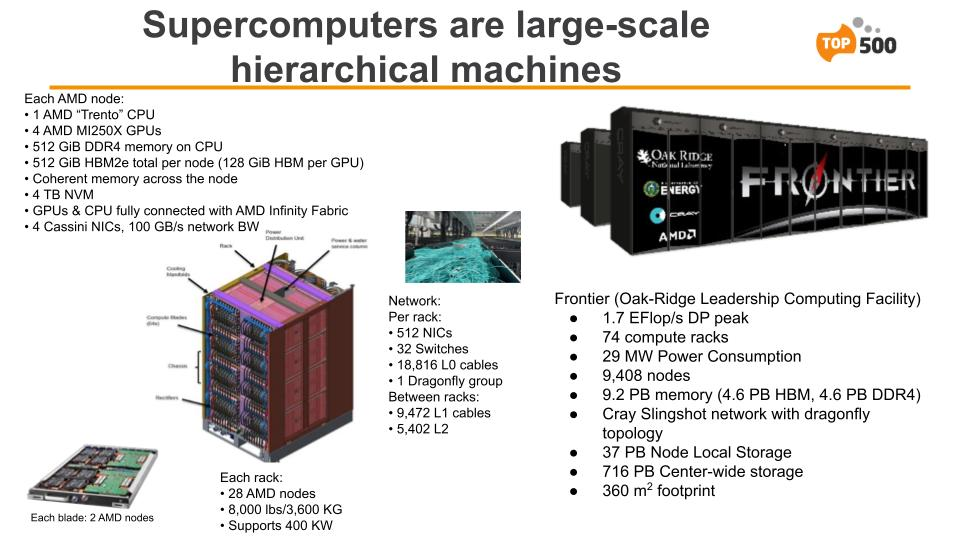
\includegraphics[width=\textwidth]{figures/frontier-architecture.jpg}

  \begin{overlayarea}{\linewidth}{0cm}
    \only<2>{%
      \vspace{-8cm}
      \begin{center}
        \begin{minipage}{.7\linewidth}
          \begin{block}{What are those system used for?}
            Scientific simulation and computing
            
            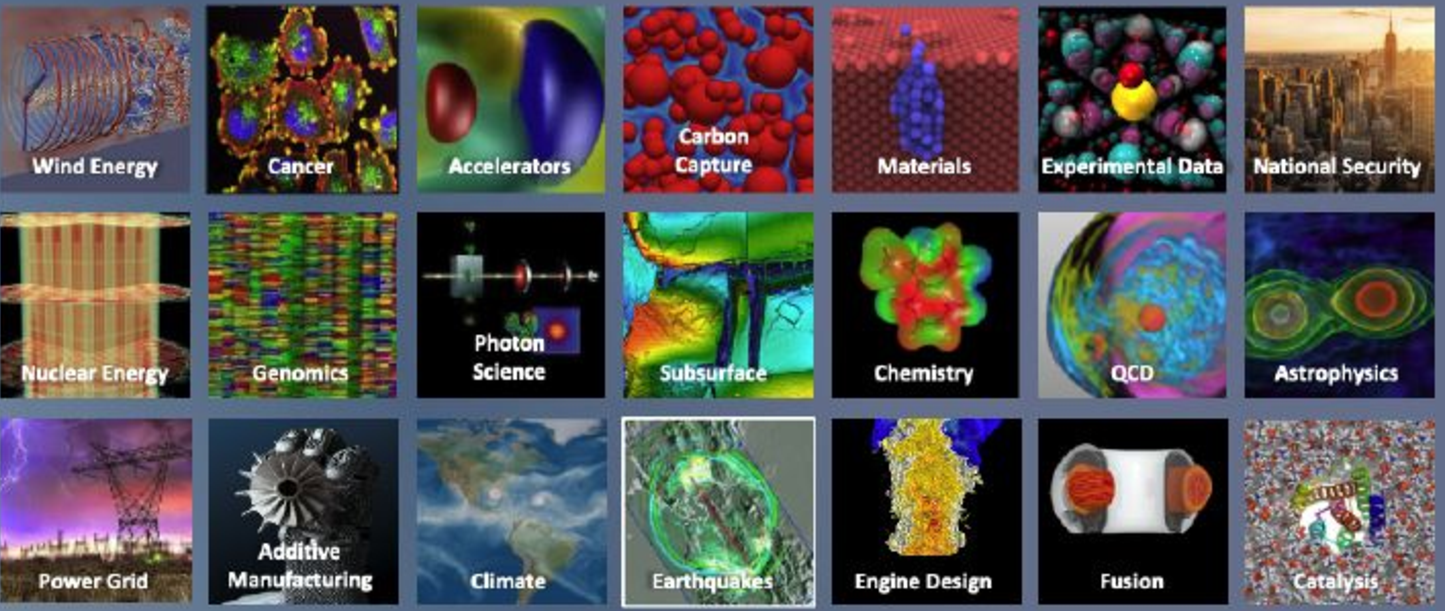
\includegraphics[width=\linewidth]{figures/hpc-applications.png}
          \end{block}
        \end{minipage}
      \end{center}
    }
  \end{overlayarea}
}

\frame{
  \includegraphics[width=\textwidth]{figures/top500.jpg}
}

\frame{
  \frametitle{Focus of this talk}

  Resilience techniques for High Performance Computing
  \begin{itemize}
  \item Rollback-recovery protocols
    \begin{itemize}
    \item Coordinated rollback-recovery
    \item Noncoordinated rollback-recovery
    \item Hierarchical protocols
    \end{itemize}
  \item Application-specific fault-tolerance
    \begin{itemize}
    \item User-Level Failure Mitigation
    \item Failure detection and notification for HPC
    \item Early Returning Agreement for ULFM
    \end{itemize}
  \end{itemize}
}

\frame{
  \frametitle{Effect of Scale}

  \begin{center}
    \only<1>{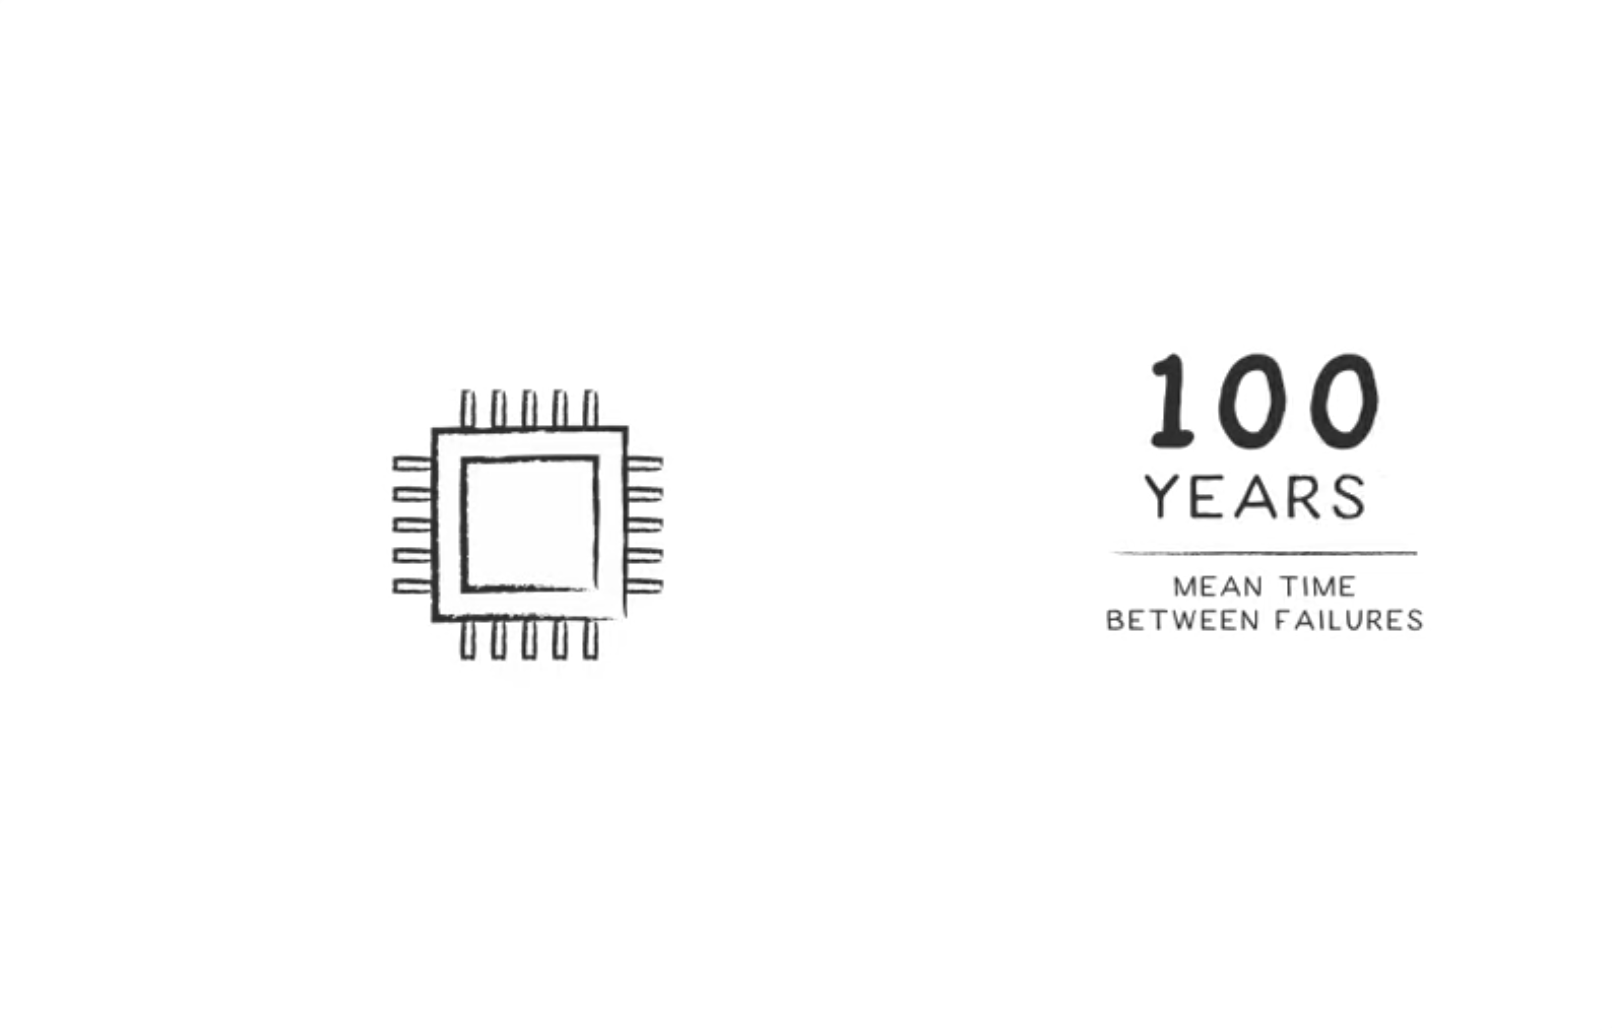
\includegraphics[width=.8\linewidth]{1_socket.png}}
    \only<2>{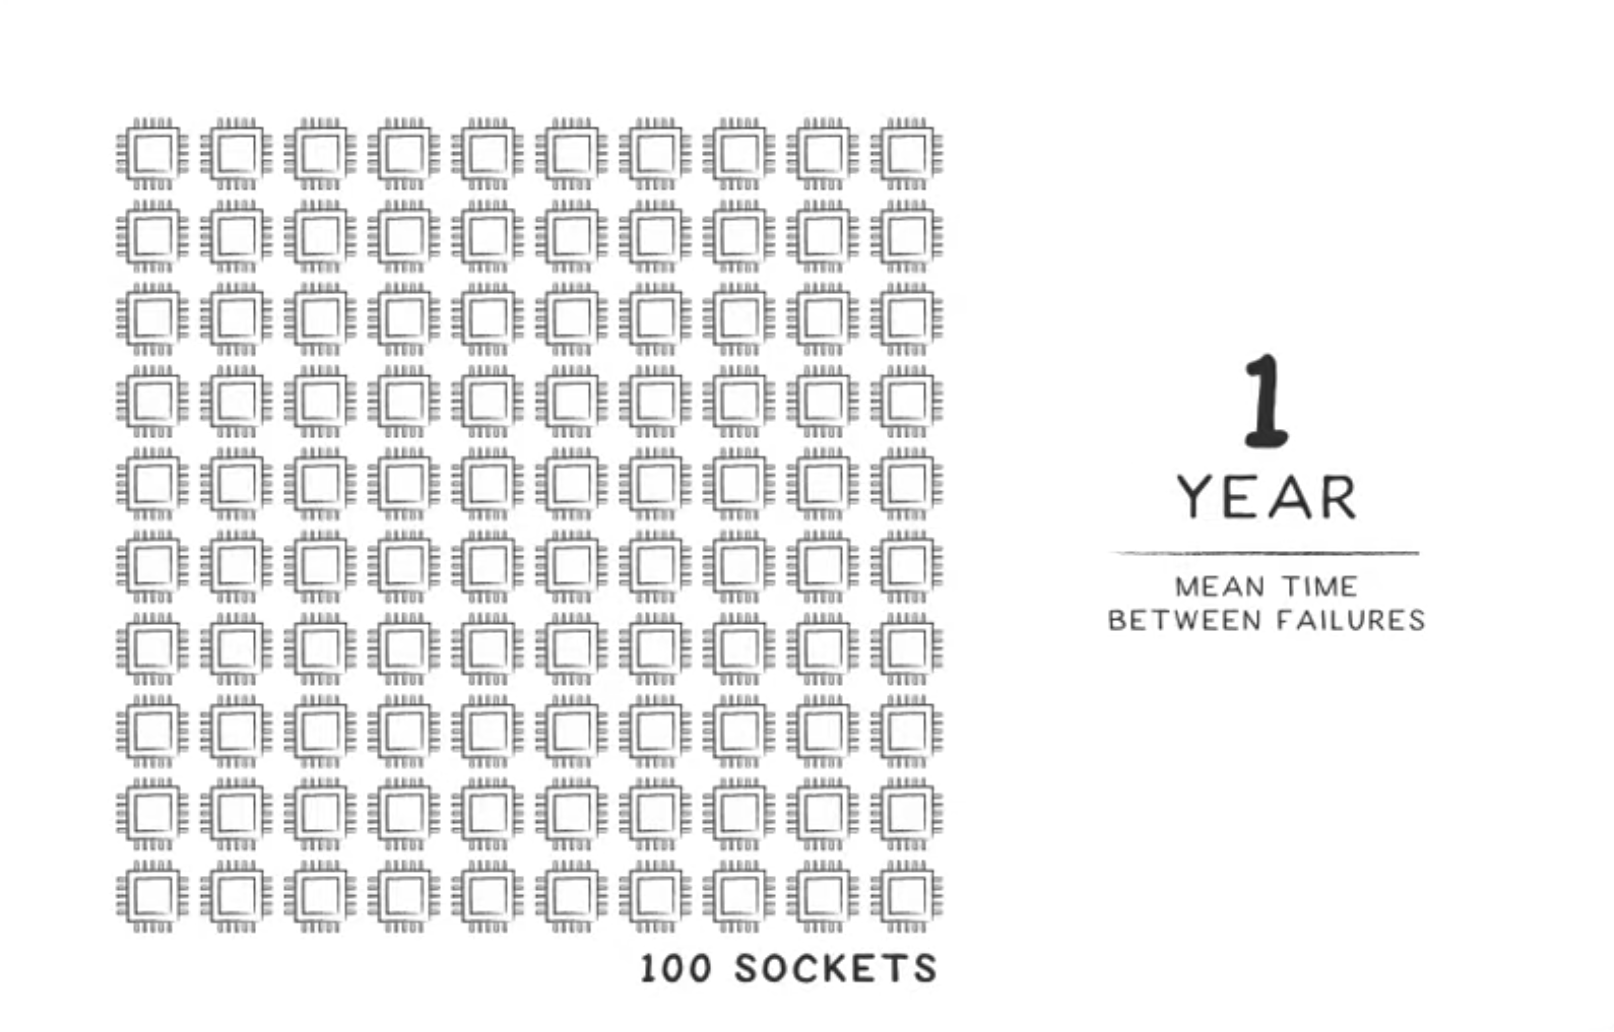
\includegraphics[width=.8\linewidth]{100_sockets.png}}
    \only<3>{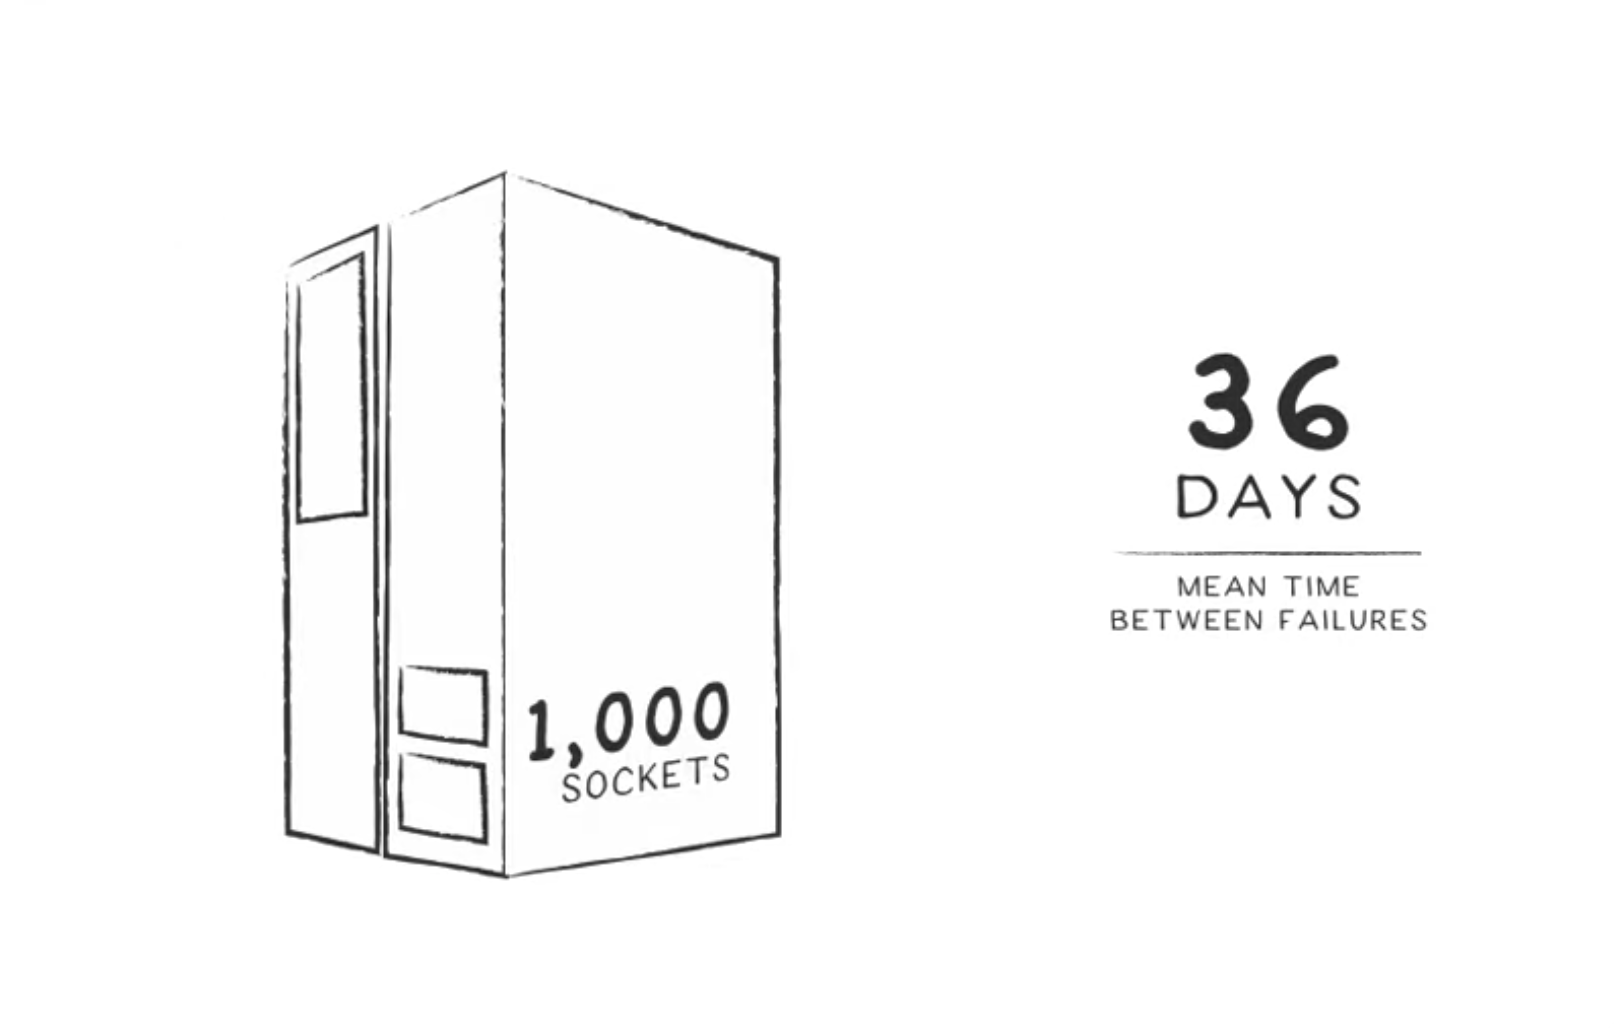
\includegraphics[width=.8\linewidth]{1000_sockets.png}}
    \only<4>{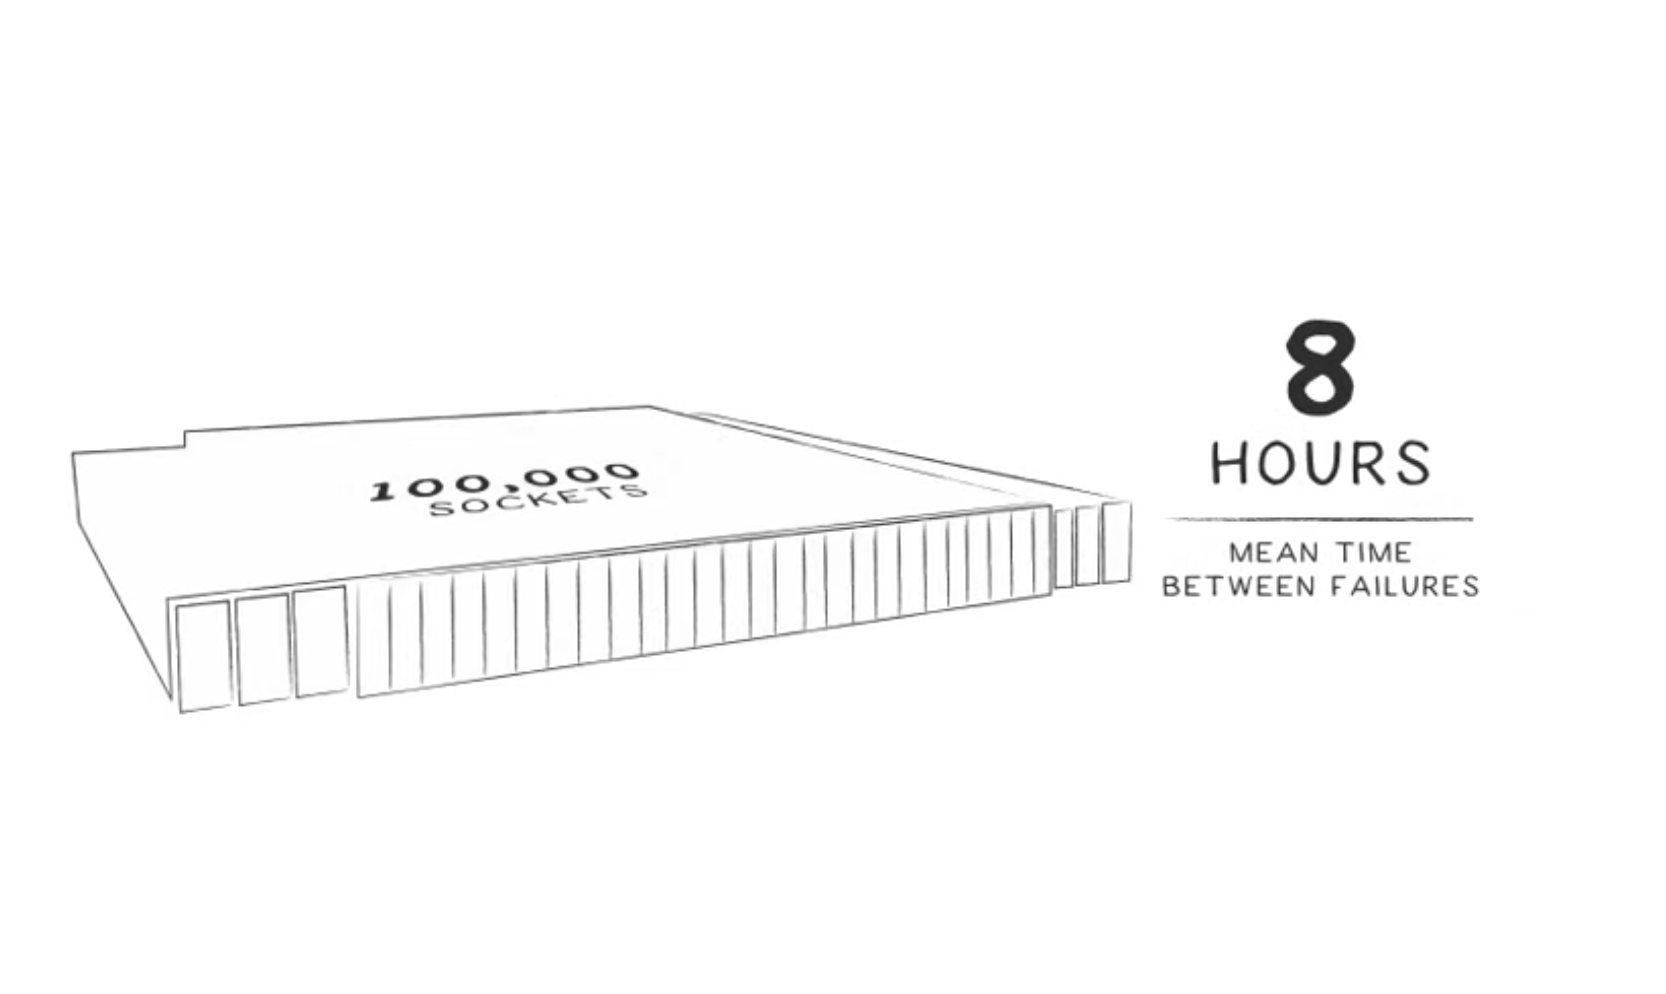
\includegraphics[width=.8\linewidth]{100000_sockets.png}}
  \end{center}
}

\frame{
  \frametitle{Petascale Computing Platforms}

  \begin{center}
    \includegraphics[width=.8\linewidth]{top500.jpg}
  \end{center}

    \begin{overlayarea}{\linewidth}{0cm}
    \only<2>{%
      \vspace{-6cm}
      \begin{center}
        \begin{minipage}{.7\linewidth}
          \begin{block}{Few Studies on the reliability of Petascale Systems}
            Not many traces and studies of Large-scale Computing Platforms
            reliability

            Not all studies look at simple characteristics (\emph{e.g.},
            MTBF):
            {\footnotesize\begin{itemize}
            \item Only \emph{Applications} failures
            \item Only \emph{Hardware} failures
            \item \emph{Logged events}
            \end{itemize}}
          \end{block}
        \end{minipage}
      \end{center}
    }
  \end{overlayarea}%
}

\frame{
  \frametitle{Petascale Platforms -- K-Computer}

  \begin{textblock*}{10cm}(0.5cm,1cm)
    \begin{block}{}
      \footnotesize \#20 Top500 (June'19, Rmax = 10.510 PFlop/s);
     06/11 --- 08/19\\
     864 cabinets; 88,128 nodes; 705,024 cores; 1.34PBytes; 12.6 MW; 
    \end{block}
    
    \vspace*{-1em}

    \begin{exampleblock}{}
     \footnotesize \emph{Fumiyoshi Shoji, Shuji Matsui, Mitsuo Okamoto, Fumichika Sueyasu,
      Toshiyuki Tsukamoto, Atsuya Uno and Keiji Yamamoto.} \textbf{ Long term
      failure analysis of 10 petascale supercomputer}.  Poster at ISC'15
    \end{exampleblock}
  \end{textblock*}

  \begin{textblock*}{4cm}(11.5cm,1.2cm) % {block width} (coords)
    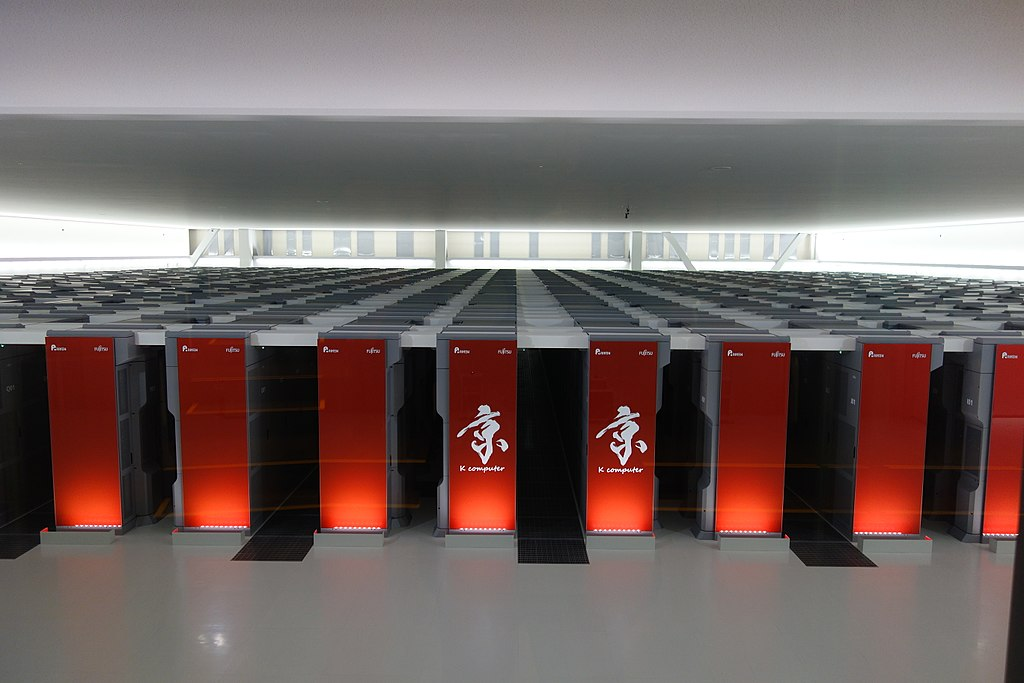
\includegraphics[width=4cm]{K-computer.jpg}
  \end{textblock*}

  \begin{textblock*}{.45\linewidth}(.02\linewidth,4.5cm)
    \small MFR = Monthly Failure Rate\\
    $\quad\qquad (= \frac{\textrm{\#failures during month}}{\textrm{\#unit total}})$

    \medskip

    \begin{tabular}{lccc}
      CPU MFR & $0.004\%$ &$\rightleftharpoons$ & $0.017\%$ \\
      DIMM MFR & $0.0017\%$ & $\searrow$ & $0.001\%$ \\
      Sys. Board MFR & $0.16\%$ & $\searrow$ & $0.05\%$\\
      \textcolor{red!40}{Sys. Board MTBF} & \textcolor{red!40}{1.1 day} & \textcolor{red!40}{$\nearrow$} & \textcolor{red!40}{3 day} \\
      \end{tabular}
  \end{textblock*}

  \begin{textblock*}{.45\linewidth}(.6\linewidth,4.5cm)
    \small AFR = Annualized Failure Rate\\
    $\quad\qquad (= 1-e^{\frac{-1 year}{MTBF}})$

    FIT = Failure In Time = \#fail. / $10^9$ h

    \bigskip

    \begin{tabular}{lcccc}
              & \# Parts & AFR & \textcolor{red!40}{MTBF} & FIT \\
      CPU & 82,944 & 0.06\% & \textcolor{red!40}{7.33 days} & 72.00 \\
      DIMM & 663,552 & 0.0016\% & \textcolor{red!40}{34.4 days} & 18.02 \\
      \end{tabular}
  \end{textblock*}

  \begin{textblock*}{.6\textwidth}(.58\textwidth,7.8cm)
    \scriptsize \textcolor{red!40}{(Numbers in red are derived from reported numbers in black)}
  \end{textblock*}
% K-computer: failure logs, CPU failures, DIMM failures, Storage
% Failures.
%   https://www.r-ccs.riken.jp/en/wp-content/uploads/sites/2/2015/11/Presentation.pdf
%  Monthly Failure Rate = Falilure count during month / number of installed (CPU|DIMM|SystemBoard)
%  CPUs Monthly failures: between 0.004% and 0.017%. Peaks at Gordon-Bell Challenges
%  DIMM Monthly failures: 0.0017% -> 0.0010% (air conditioner operations got improvement)
%  System Board MF: started at 0.16% decreased to 0.05%
%  Comparison with Blue Waters:
%    AFR = Annual Failure Rate -> K-computer 0.06%, Blue Waters 0.23%
%    FIT: Failure In Time (1 FIT = 1 failure per 10^9 hours of
%    computation on entire platform) -> K-computer 72, Blue Waters
%    265.15
%  For Blue waters see C. Di Martino et al., Lessons learned from the
%  analysis of system failures at petascale: the case of blue
%  waters. 44th international conference on Dependable Systems and
%  Networks (DSN 2014), 2014. 
%  System Availability: 93.59%, 4.19% scheduled maintenance, 2.23%
%  system failure.
%  Root cause: 1.38%/2.23% of file system.

}

\frame{
  \frametitle{Petascale Platforms -- Titan}

  \begin{textblock*}{10cm}(0.5cm,1cm)
    \begin{block}{}
      \footnotesize \#12 Top500 (June'19, Rmax = 17.590 PFlop/s);
     10/12 --- 08/19\\
     200 cabinets; 18,688 nodes; 299,008 cores; 18,688  K20X; 693.6TBytes; 8.2 MW; 
    \end{block}
  \end{textblock*}
    
  \begin{textblock*}{15cm}(0.5cm,2.5cm)
    \begin{exampleblock}{}
     \footnotesize \emph{R. A. Ashraf and C. Engelmann,} \textbf{Analyzing the
     Impact of System Reliability Events on Applications in the Titan
     Supercomputer}, 8th Workshop on Fault Tolerance for
     HPC at eXtreme Scale (FTXS), 2018
    \end{exampleblock}
  \end{textblock*}

  \begin{textblock*}{4cm}(11.5cm,1.2cm) % {block width} (coords)
    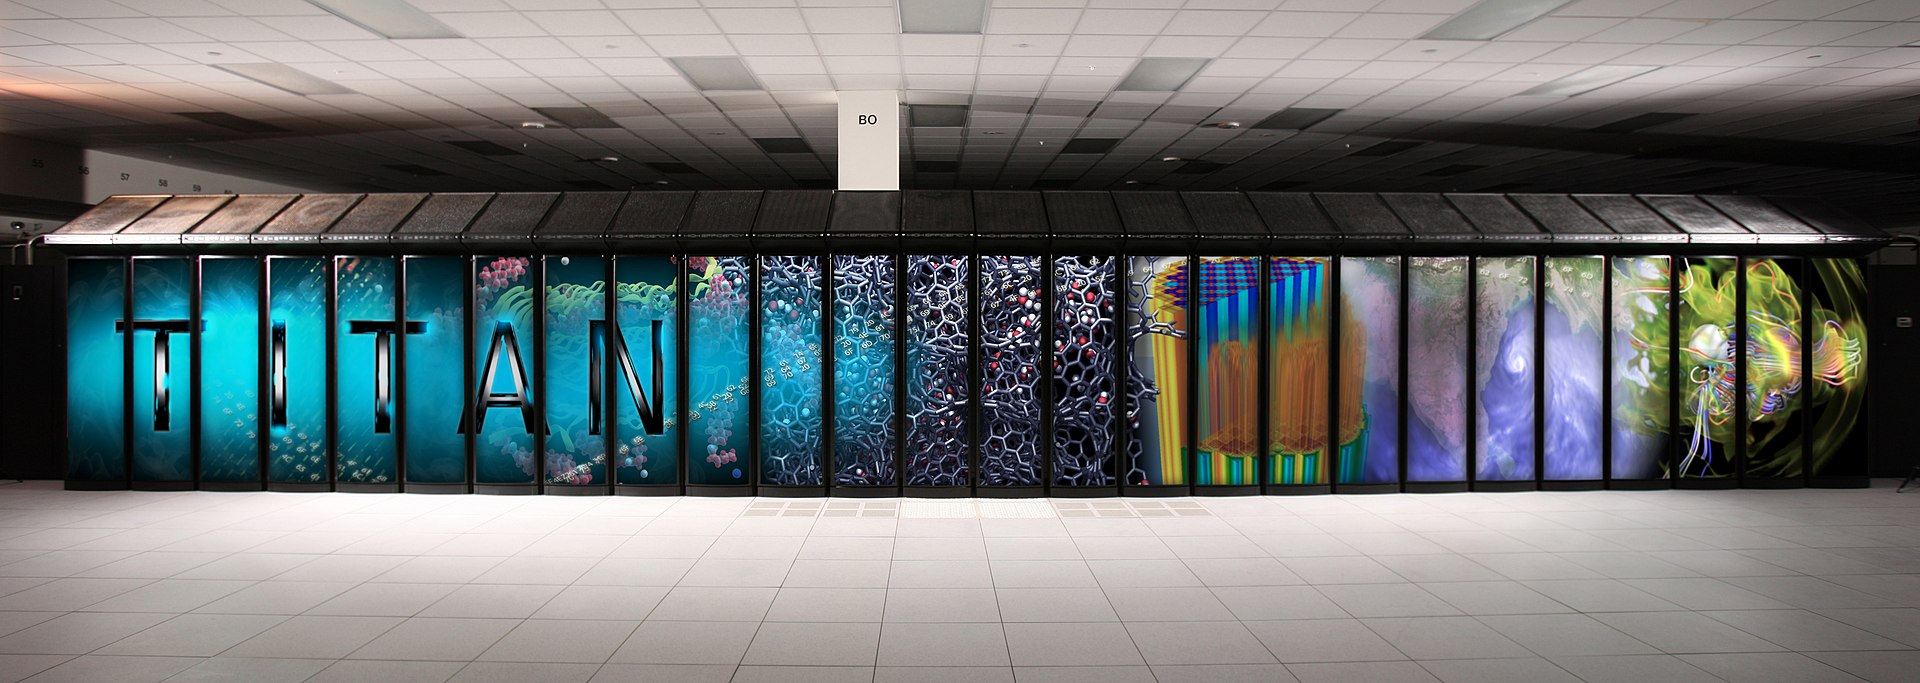
\includegraphics[width=4cm]{Titan.jpg}
  \end{textblock*}

  \begin{textblock*}{.5\linewidth}(.02\linewidth,4cm)
    Event log from Reliability, Availability and Serviceability (RAS)
    System

    \medskip
    $68k$ apps have $1+$ events (over $2\cdot 10^6$)

    \medskip\small
    95\% of apps with 11k+ nodes have $1+$ events

    91\% of apps with 125- nodes have 0 events

    85\% apps under 30min have 0 events

    80\% apps above 24h have $1+$ events
  \end{textblock*}

  \begin{textblock*}{.45\linewidth}(.6\linewidth,4cm)
    Nature of first event hitting an application:
    \begin{tabular}{ll}
      Parallel Filesystem & 73.7\%\\
      Processor Failure & 15.7 \%\\
      Machine Check Exception & 6.5\%\\
      GPU Failure & 1.5\%\\
      OOM / SEGFAULT & 1.9\%\\
      Interconnect & 0.8 \%
    \end{tabular}
  \end{textblock*}

% Titan Reliability
%   https://ieeexplore.ieee.org/abstract/document/8564486
% Evaluate events from RAS (Reliability, Availability and
% Serviceability) system. Eevents might not denote failure of 
% job. 68k applications / 2 million had an event reported.
% Events are also correlated: a FS failure often translates into a MCE
% failure and/or a Processor failure. GPU failure also, etc.
%   First event distribution:
%     Parallel FS: 73.7% of errors
%     Processor failures: 15.7%
%     Machine Check Exception (this includes masked failures, like
%     corrected ECC): 6.5%
%     GPU: 1.5%
%     OOM / SEGFAULT: 1.9%
%     Interconnect: 0.8%
%  95% of apps with 11250 to max nodes reported at least an event;
%  91% of apps in the 1 to 125 job size bin reported no event.
%  Similar story about duration: 85% of apps that are below 30min
%  reported no event 80% of apps above 24h reported an event
% 
}

\frame{
  \frametitle{Petascale Platforms -- Titan}

  \begin{textblock*}{10cm}(0.5cm,1cm)
    \begin{block}{}
      \footnotesize \#12 Top500 (June'19, Rmax = 17.590 PFlop/s);
     10/12 --- 08/19\\
     200 cabinets; 18,688 nodes; 299,008 cores; 18,688  K20X; 693.6TBytes; 8.2 MW; 
    \end{block}
  \end{textblock*}
    
  \begin{textblock*}{15cm}(0.5cm,2.5cm)
    \begin{exampleblock}{}
     \footnotesize \emph{E. Rojas, E. Meneses, T. Jones and D. Maxwell} \textbf{Analyzing a Five-year Failure Record of a
Leadership-class Supercomputer}, 31st Intl. Symp. on Computer Architecture and HPC (SBAC-PAD), 2019
    \end{exampleblock}
  \end{textblock*}

  \begin{textblock*}{4cm}(11.5cm,1.2cm) % {block width} (coords)
    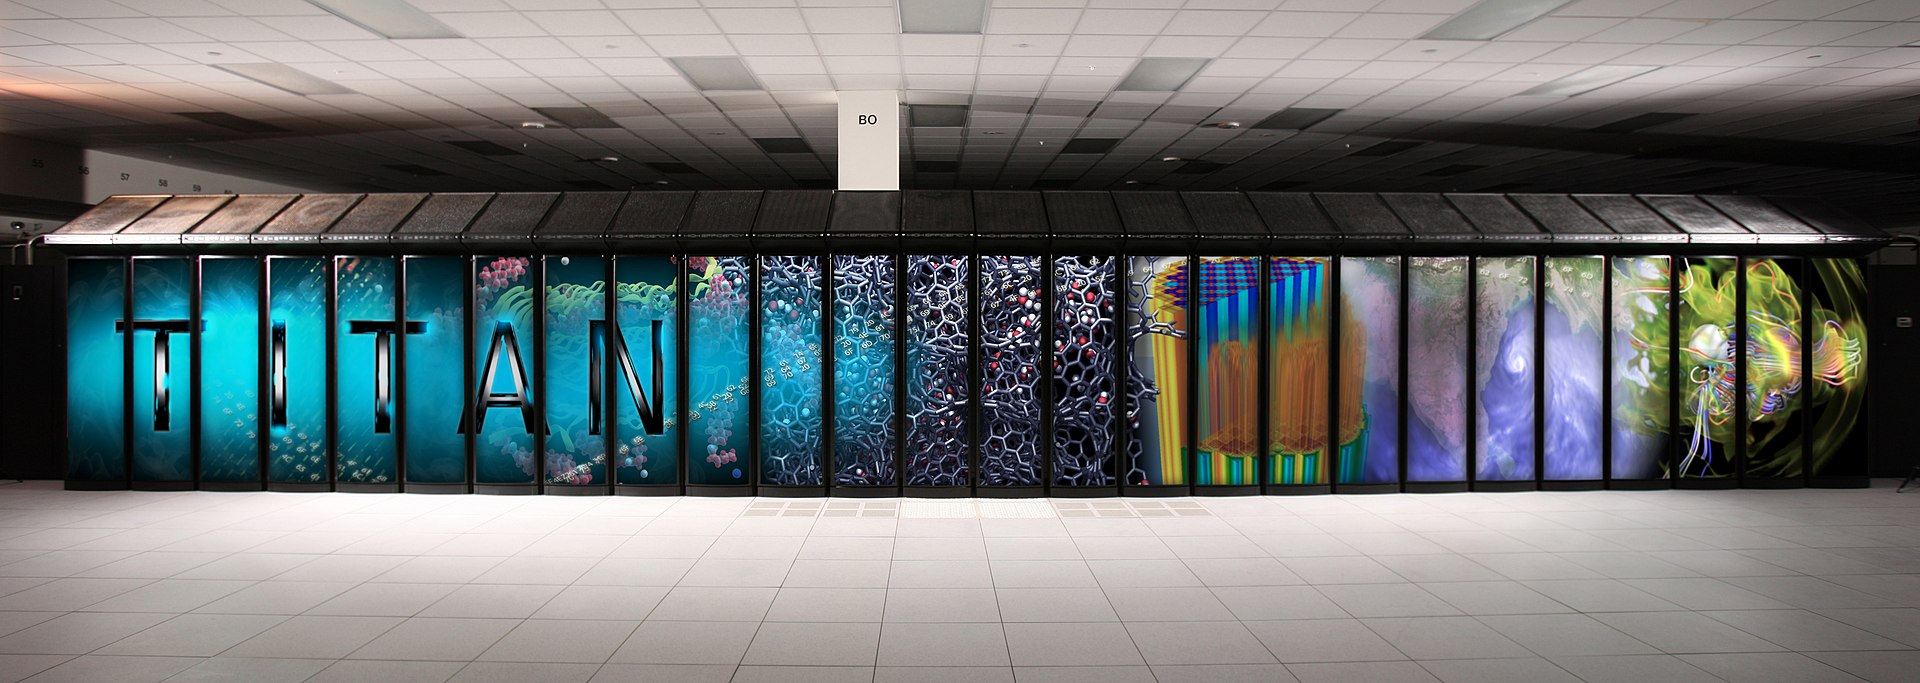
\includegraphics[width=4cm]{Titan.jpg}
  \end{textblock*}

  \begin{textblock*}{.5\linewidth}(.02\linewidth,4cm)
    System failure database (sys. admin.)

    {\small
    \begin{tabular}{c|ccccc}
      Year & 2014 & 2015 & 2016 & 2017 & 2018\\\hline
      Events & 161k & 258k & 444k & 452k & 1,348k \\\hline
    \end{tabular}}
    {\tiny (About 30\% of events are categorized as having a user origin)}

    \medskip
    %Several (potentially many) events may represent a single failure.
    5,625 hardware failures / 4 years ($\approx$4/day -- \textcolor{red!40}{6h MTBF})\\

    %\medskip
    %816,826 events (30.7\%) categorized as user, removed from the
    %analysis

    \medskip
    GPU DBE represents 53\% of hardware events
    {\small
    ECC on these GPUs
    is single error correction double error detection, leads to interrupt
    in DBE.}
 \end{textblock*}

  \begin{textblock*}{.45\linewidth}(.6\linewidth,4cm)
    Nature of failure:
    \begin{tabular}{ll}
      GPU DBE & 2070 (37\%)\\
      GPU BUS & 797 (14\%)\\
      GPU DPR & 308 (5.5\%)\\
      GPU XID (Soft.) & 1370 (24\%)\\
      Machine Check Exc & 653 (12\%)\\
      Other Failures & 427 (7.5\%)
    \end{tabular}
  \end{textblock*}

  \begin{textblock*}{.6\textwidth}(.58\textwidth,7.8cm)
    \scriptsize \textcolor{red!40}{(Numbers in red are derived from reported numbers in black)}
  \end{textblock*}

% Titan Reliability 2
%   https://ieeexplore.ieee.org/stamp/stamp.jsp?tp=&arnumber=8924181
% Evaluate events from a database of errors collected between 2014 and 2018.
% Correlate with jobs database and return code, and separate system errors
% from user errors.
%  68k applications / 2 million had an event reported.
% Events are also correlated: a FS failure often translates into a MCE
% failure and/or a Processor failure. GPU failure also, etc.
%   First event distribution:
%     Parallel FS: 73.7% of errors
%     Processor failures: 15.7%
%     Machine Check Exception (this includes masked failures, like
%     corrected ECC): 6.5%
%     GPU: 1.5%
%     OOM / SEGFAULT: 1.9%
%     Interconnect: 0.8%
%  95% of apps with 11250 to max nodes reported at least an event;
%  91% of apps in the 1 to 125 job size bin reported no event.
%  Similar story about duration: 85% of apps that are below 30min
%  reported no event 80% of apps above 24h reported an event
% 
}


\begin{frame}
  \frametitle{Petascale Platforms -- Sunway TaihuLight}

  \begin{textblock*}{10cm}(0.5cm,1cm)
    \begin{block}{}
      \footnotesize \#3 Top500 (June'19, Rmax = 93.014 PFlop/s);
     06/16 --- \\
     40 cabinets; 20,480 nodes; 10,649,600 cores; 1.32PBytes; 15 MW; 
    \end{block}
  \end{textblock*}
    
  \begin{textblock*}{10cm}(0.5cm,2cm)
    \begin{exampleblock}{}
     \footnotesize \emph{Liu RT, Chen ZN.} \textbf{A large-scale study of failures on
     petascale supercomputers.} Journal of Computer Science and
   Technology 33(1): 24-41, Jan. 2018
    \end{exampleblock}
  \end{textblock*}

  \begin{textblock*}{4cm}(11.5cm,1.2cm) % {block width} (coords)
    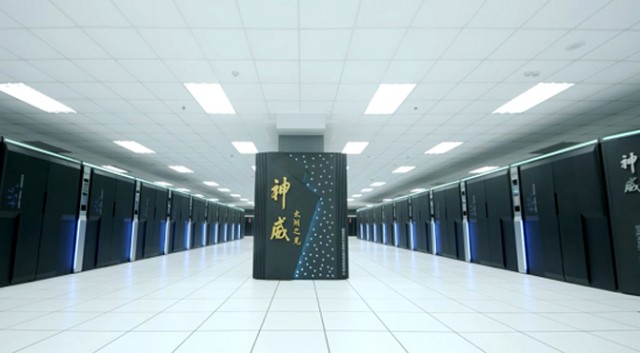
\includegraphics[width=4cm]{taihulight.jpg}
  \end{textblock*}

  \begin{textblock*}{.5\linewidth}(.02\linewidth,4cm)
    \footnotesize Nature of faults:
    \begin{tabular}{lll}
                & All Failures & Fatal Failures\\
      CPU       & 40\%         & 68\% \\
      Memory    & 48\%         & 21\% \\
      Power     & 9\%          & 5\%\\
      MD$^{(*)}$ & 2\%          & 5\% \\
    \end{tabular}

    {\scriptsize ($(*)$ MD: Maintenance and Diagnosis system)}

    \medskip
    Effect of Application (1 cabinet, \#faults/month):
    \begin{tabular}{lll}
                     & Mem Faults                   & CPU Faults \\
        Comp. only   & $7 \rightleftharpoons 93$    & $5 \rightleftharpoons 33$ \\
        Comp. \& Mem & $527 \rightleftharpoons 995$ & $136 \rightleftharpoons 867$ \\
        Comm. \& Mem & $115 \rightleftharpoons 284$ & $20 \rightleftharpoons 85$
    \end{tabular}
  \end{textblock*}

  \begin{textblock*}{.45\linewidth}(.6\linewidth,4cm)
    {\small 3 time spans; 1 CPU; 2 Computing Cards}
    Weibull Distribution best fits CDF

    \medskip
    \begin{tabular}{llll}
                    & $P_1$    & $P_2$  & $P_3$ \\
      $CPU_1$ MTBF  & 8 days   & 4 days & 10 days\\
      $Card_1$ MTBF & 9.5 days &        & \\
      $Card_2$ MTBF & 10 days  &        & \\
    \end{tabular}

    \medskip
    {\scriptsize\textcolor{red!40}{Data too sparse to give a system MTBF}}\\
    {\scriptsize\textcolor{red!40}{It was probably small}}
        
    {\tiny MTBF computed from $\eta$ and $m$ parameters
      given in the article:\\
      PDF: $f(x) = \frac{m}{\eta}(\frac{x}{\eta})^{m-1}e^{-(x/\eta)^m}$;\\
      MTBF: $=\eta\, \Gamma(1+1/m)$}
    
  \end{textblock*}

% A large scale study of failures on petascale supercomputers (2018):
% https://link.springer.com/content/pdf/10.1007%2Fs11390-018-1806-7.pdf
%  Sunway BlueLight (based on multi-core CPUs) and Sunway TaihuLigh
%  (based on heterogeneous manycore CPUs
% They conclude that a Weibull distribution always fits best both machines,
% but the parameters depends strongly on the workload. For example, on 
% CPU failures, for Sunway TaihuLigh they take 3 random intervals
% (epochs) and find:
%   -> MTBF = eta * Gamma(1 + 1/m) = 690434s (8 days) during 'epoch 1'
%            351001s (4 days) during 'epoch 2'
%            906820s (10 days) during 'epoch 3'
% Looking at the interconnect level, they find a Time Between Failure
%  between 824082.3s (9.5 days) and 9.08.10^5s (10 days).
%  Sunway BlueLigh: 91.99 of all notifications are memory events,
%    44.48% of fatal errors are due to CPU
%    41.67% of fatal errors are due to Interconnect
%    9.36% of fatal errors are due to power supply
%   Only 1.03% fatal errors are due to memory.
% Sunway TaihuLigh: 48% of nonfatal & Fatal are due to Memory, 40% are
% due to CPU, and 9% to Power
%     Fatal errors: 68% due to CPU, 21% to memory 5% to power
%
\end{frame}

\begin{frame}
  \frametitle{In the recent past}
  
  \begin{center}
    \relsize{-1}
    \begin{tabular}{l|l|l|l|l|l}
      System & \#Nodes & \#cores & Period & MTBF (h) & Scale-Norm. MTBF (h) \\\hline
      Jaguar XT4 & 7,832  & 31,328  & Jan'08-Mar'11 & 36.91 & 15.47 \\\hline
      Jaguar XT5 & 18,688 & 149,504 & Jan'09-Dec'11 & 22.67 & 22.67 \\\hline
      Jaguar XK6 & 18,688 & 298,592 & Jan'12-Oct'12 & 8.93  &  8.93 \\\hline
      Eos XC 30 & 736     & 23,553  & Sep'13-Sep'15 & 189.04 & 7.45 \\\hline
      Titan XK7 & 18,688  & 560,640 & May'13-Sep'15 & 14.51  & 14.51 \\
    \end{tabular}

    \medskip

    \relsize{-1} Table 2 + 3 of ``Failures in Large Scale Systems: Long-term Measurement, Analysis, and Implications'',\\
    by S. Gupta, T. Patel, C. Engelmann, and D. Tiwari, SC'17
  \end{center}

  \bigskip

  \noindent$\bullet$ Reliability does not seem to be correlated with size or 'age' of the machine\\
  $\bullet$ A few failure types constitute a major fraction of all failures.\\
  $\bullet$ Temporal recurrences are observed
  
\end{frame}

\frame{
  \frametitle{Exascale platforms (courtesy Jack Dongarra)}

  \centerline{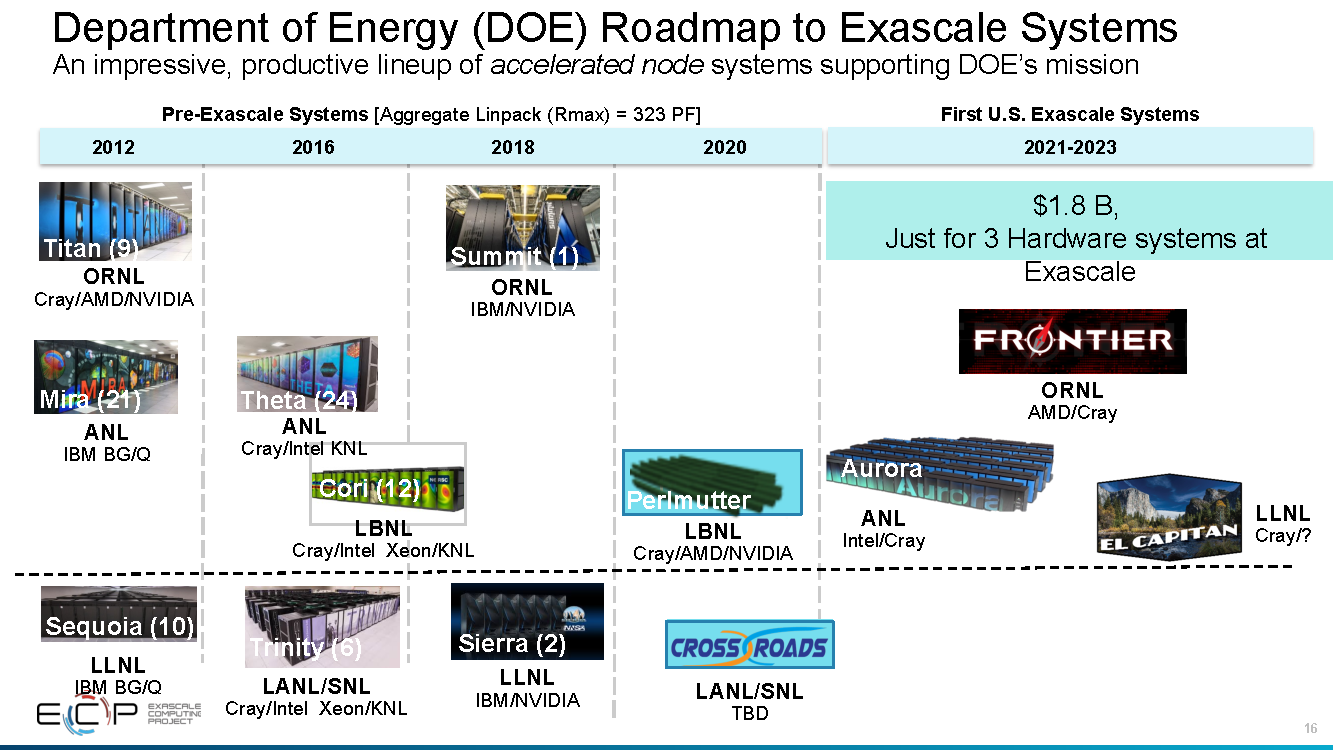
\includegraphics[width=1.4\textheight]{DOE-Exascale-Roadmap.pdf}}

  \begin{overlayarea}{\linewidth}{0cm}
    \only<2>{%
      \vspace{-6cm}
      \begin{center}
        \begin{minipage}{.7\linewidth}
          \begin{block}{Fewer Studies on the reliability of Pre-Exascale Systems}

            \begin{itemize}
            \item MTBF of \textcolor{blue}{systems} appear to remained capped
            \item \# nodes in Top10 has \emph{decreased}
            \item Computing power of nodes has significantly increased thanks to \emph{many GPUs} / node
              \begin{itemize}
              \item Notable exceptions:
              \item[] $\qquad$ K-Computer, Fugaku
              \item[] $\qquad$ Sunway *light
              \end{itemize}
            \end{itemize}
          \end{block}
        \end{minipage}
      \end{center}
    }
  \end{overlayarea}%

}


\section{Checkpointing Protocols}

\def\smiley{\green{\larger[2]\wasyfamily\char44}\xspace}
\def\frownie{\blue{\larger[2]\wasyfamily\char47}\xspace}
\def\quesley{\yyellow{\hbox to -0.08em{\textraiseglotstop}$_{\textrm{\wasyfamily\char47}}$}\xspace}

\newtheorem{proposition}{Proposition}
%\newtheorem{corollary}{Corollary}
%\newtheorem{definition}{Definition}
%\newtheorem{remark}{Remark}

%% Macros - hierarchical paper
\newcommand{\wastecoordnofail}{\ensuremath{\textsc{Waste}_{\mathit{coord-nofailure}}}}
\newcommand{\wastecoordfail}{\ensuremath{\textsc{Waste}_{\mathit{coord-failure}}}}
\newcommand{\overheadcoordfail}{\ensuremath{\Overhead_{\mathit{coord}}}}
\newcommand{\wastecoordfailinw}{\ensuremath{\textsc{Waste}_{\mathit{coord-fail-in-work}}}}
\newcommand{\overheadcoordfailinw}{\ensuremath{\Overhead_{\mathit{coord-fail-in-work}}}}
\newcommand{\wastecoordfailinc}{\ensuremath{\textsc{Waste}_{\mathit{coord-fail-in-checkpoint}}}}
\newcommand{\overheadcoordfailinc}{\ensuremath{\Overhead_{\mathit{coord-fail-in-checkpoint}}}}
\newcommand{\wastecoord}{\ensuremath{\textsc{Waste}_{\mathit{coord}}}}
\newcommand{\wckpt}{\textsc{waste}_{ckpt}}
\newcommand{\ockpt}{\Overhead_{ckpt}}
\newcommand{\ocomp}{\Overhead_{comp}}
\newcommand{\wbckpt}{\textsc{waste}_{before\_ckpt}}
\newcommand{\obckpt}{\Overhead_{before\_ckpt}}
\newcommand{\wdckpt}{\textsc{waste}_{during\_ckpt}}
\newcommand{\odckpt}{\Overhead_{during\_ckpt}}
\newcommand{\wackpt}{\textsc{waste}_{after\_ckpt}}
\newcommand{\oackpt}{\Overhead_{after\_ckpt}}
\newcommand{\avgwckpt}{\textsc{avg\_waste}_{ckpt}}
\newcommand{\avgockpt}{\textsc{avg\_\Overhead}_{ckpt}}
\newcommand{\qmin}{\ensuremath{\text{q}_{\min}}\space}%cpu frequency
\newcommand{\StenTwo}{\textsc{2D-Stencil}\xspace}
\newcommand{\StenThree}{\textsc{3D-Stencil}\xspace}
\newcommand{\Matprod}{\textsc{Matrix-Product}\xspace}
\newcommand{\CSCI}{\textsc{Coord-IO}\xspace}
\newcommand{\CSHI}{\textsc{Hierarch-IO}\xspace}
\newcommand{\CSHIPlane}{\textsc{Hierarch-IO-Plane}\xspace}
\newcommand{\CSHILine}{\textsc{Hierarch-IO-Line}\xspace}
\newcommand{\CSCP}{\textsc{Coord-Port}\space}
\newcommand{\CSHP}{\textsc{Hierarch-Port}\xspace}
\def\PP{\mathbb{P}}
\newcommand{\Topt}{\mathbb{T}^*}
\newcommand{\XX}{C}
\newcommand{\Work}{\textsc{Work}}
\newcommand{\Overhead}{\textsc{Re-Exec}}
\newcommand{\Waste}{\textsc{Waste}}
\newcommand{\Useful}{\textsc{UsefulFraction}}
\newcommand{\coord}{\text{coord}}
\newcommand{\hierarch}{\text{hierarch}}
\newcommand{\cmem}{C_{\text{Mem}}}
\newcommand{\Wastecoordopt}{{\Waste_{coord}}^*}
\newcommand{\ngroups}{\ensuremath{G}\xspace} %Number of groups in platform
\newcommand{\nsubgroups}{\ensuremath{H}\xspace} %Number of sub-groups in a group for port-saturated
\newcommand{\vgroups}{\ensuremath{g}\xspace} %Variable to iterate on groups
\newcommand{\muplatform}{\ensuremath{\mu}\xspace} %MTBF of platform
\newcommand{\nprocess}{\ensuremath{p_{total}}\xspace} %Number of processors in platform
\newcommand{\nprocessR}{\ensuremath{N}\xspace} %Number of processors in platform
\newcommand{\vsegment}{\ensuremath{s}\xspace} %Variable to iterate on segments
\newcommand{\nq}{\ensuremath{q}\xspace} %Number of processors in a group
\newcommand{\cplatform}{\ensuremath{C}\xspace} %checkpoint de la platforme
\newcommand{\rplatform}{\ensuremath{R}\xspace} %recovery de la platforme
\newcommand{\dplatform}{\ensuremath{D}\xspace} %downtime de la platforme
\newcommand{\cgroup}{\ensuremath{C(\nq)}\xspace} %checkpoint d'un groupe
\renewcommand{\rgroup}{\ensuremath{R(\nq)}\xspace} %recovery d'un groupe
\newcommand{\dgroup}{\ensuremath{D(\nq)}\xspace} %downtime d'un groupe
\newcommand{\W}{\ensuremath{W}\xspace}% travail utile
\newcommand{\T}{\ensuremath{T}\xspace} % 'Checkpoint' interval
\newcommand{\amountlog}{\ensuremath{\beta}\xspace}%Amount of logging per time unit
\newcommand{\workduringckpt}{\ensuremath{\alpha}\xspace}%Ratio of the checkpointing time that can be used as work
\newcommand{\cgroupbase}{\ensuremath{C_0(\nq)}\xspace}%Time to save the group without message logging
\newcommand{\dgroupbase}{\ensuremath{D_0(\nq)}\xspace}%Time to save the group without message logging
\newcommand{\rgroupmin}{\ensuremath{R_0(\nq)}\xspace}%Time to recover the group without message logging
\newcommand{\rgroupbase}{\ensuremath{R_0(\nq)}\xspace}%Time to save the group without message logging
\newcommand{\MFPA}{\ensuremath{\text{Mem}}\xspace}%memory footprint
\newcommand{\bwio}{\ensuremath{\text{b}_{io}}\xspace}%i/o bandwidth
\newcommand{\bwnode}{\ensuremath{\text{b}_{port}}\xspace}%inode/port bandwidth
\newcommand{\speed}{\ensuremath{\text{s}_{p}}\xspace}%cpu frequency

\newcommand{\opt}{\ema{{\text{opt}}}}
%% Macros - prediction
\newcommand{\C}{C\xspace}
\newcommand{\CC}{C\xspace}
\newcommand{\D}{D\xspace}
\newcommand{\R}{R\xspace}
\newcommand{\p}{p\xspace}
\newcommand{\q}{q\xspace}
\newcommand{\qopt}{q_{opt}}
\newcommand{\recall}{\ensuremath{r}\xspace}
\newcommand{\precision}{\ensuremath{p}\xspace}
\newcommand{\trust}{\ensuremath{q}\xspace}
\newcommand{\muP}{\ensuremath{\mu_{P}}\xspace}
\newcommand{\muNP}{\ensuremath{\mu_{NP}}\xspace}
\newcommand{\munew}{\ensuremath{\mu_e}\xspace}
\newcommand{\period}{\ensuremath{T}\xspace}

%% Macros - Dounia FTXS
\def\e{\mathop{\rm e}\nolimits}
\def\pr{\mathop{\rm Pr}\nolimits}
\def\P{\mathop{\mathbb{P}}\nolimits}
\def\E{\mathop{\mathbb{E}}\nolimits}
\def\En{\mathop{\mathbb{E}_n}\nolimits}
\def\Ew{\mathop{\mathbb{E}_w}\nolimits}
\def\EW{\mathop{\mathbb{E}_W}\nolimits}
\def\ET{\mathop{\mathbb{E}_T}\nolimits}
\def\Ep{\mathop{\mathbb{E}_p}\nolimits}
\def\Eo{\mathop{\mathbb{E}_o}\nolimits}
\def\EO{\mathop{\mathbb{E}_O}\nolimits}
\def\Eopt{\mathop{\mathbb{E}_{opt}}\nolimits}
\def\Wopt{\mathop{W_{opt}}\nolimits}
\def\Elost{\mathop{\mathbb{E}_{lost}}\nolimits}
\def\iid{\textit{iid}\xspace}
\def\Psucc{\mathop{\mathcal{P}_{\text{succ}}}\nolimits}
\def\Ewasted{\mathop{\mathbb{E}_{\text{wasted}}}\nolimits}
\def\Ewastedp{\mathop{\mathbb{E}_{\text{wasted}}}\nolimits}
\def\Topt{\ensuremath{T_{\text{opt}}}}
\def\Tcand{\ensuremath{T_{\text{cand}}}}
\def\Xp{\ensuremath{X^{(p)}}}
\newcommand{\pused}{p_{used}}
\newcommand{\Petasc}{Petascale}
\newcommand{\Exasc}{Exascale}
\newcommand{\nbfail}{n^{fail}}
%\newcommand{\s}{s}
\newcommand{\Speedup}{\mathit{loss}}
\newcommand{\Psuc}{P_{suc}}
\newcommand{\Xexec}{T}
\newcommand{\Xwork}{W}
\newcommand{\Xlost}{T_{lost}}
\newcommand{\Rlost}{R_{lost}}
\newcommand{\Xrec}{T_{rec}}
\newcommand{\Xwasted}{T_{wasted}}
\newcommand{\f}{f}
\newcommand{\talive}{\tau}
\newcommand{\w}{\omega}
\newcommand{\lamb}{\mathbb{L}} %lambert function
\newcommand{\tinit}{t^{init}}
\newcommand{\myalpha}{\alpha}
\newcommand{\mybeta}{\beta}
\newcommand{\tcst}{t^{cst}}
\renewcommand{\c}{C}
\renewcommand{\r}{R}
\renewcommand{\a}{a}
\renewcommand{\d}{D}

%% Macros replication
\newcommand{\Hopt}{\ema{\mathbb{H}_{\textit{opt}}}}
\newcommand{\nbf}{\ema{n_{\text{fail}}}}
\newcommand{\MM}{\ema{M}}
\newcommand{\bb}{\ema{b}}
\newcommand{\pg}{q}
\newcommand{\N}{N}
%\newcommand{\NFTI}{\ensuremath{\mathit{NFTI}}\xspace}
\newcommand{\NFTIkf}{\ensuremath{\mathit{NFTI}^{\mathrm{ah}}}\xspace}
\newcommand{\MNFTIbase}{\ensuremath{\mathit{MNFTI}}\xspace}
%\newcommand{\MNFTI}{\ensuremath{\mathit{MNFTI}}\xspace}
\newcommand{\MNFTIkf}{\ensuremath{\mathit{MNFTI}^{\mathrm{ah}}}\xspace}
%\newcommand{\NFTIah}{\ensuremath{\mathit{NFTI}^{\mathrm{ah}}}\xspace}
\newcommand{\NFTI}{\ensuremath{\mathit{NFTI}^{\mathrm{rp}}}\xspace}
\newcommand{\TTI}{\ensuremath{\mathit{TTI}}\xspace}
%\newcommand{\MNFTIah}{\ensuremath{\mathit{MNFTI}^{\mathrm{ah}}}\xspace}
\newcommand{\MNFTI}{\ensuremath{\mathit{MNFTI}^{\mathrm{rp}}}\xspace}
\newcommand{\MTTI}{\ensuremath{\mathit{MTTI}}\xspace}
\newcommand{\MNFTIgen}{\ensuremath{\mathit{MNFTI}}\xspace}
\newcommand{\PRR}{\textsc{Process replication}\xspace}
\newcommand{\GRR}{\textsc{Group replication}\xspace}
\newcommand{\Birthday}{\textit{Birthday}}
\newcommand{\nrep}{\ensuremath{g}\xspace} %Number of replicas in process replication
\newcommand{\nprocessrep}{\ensuremath{n_{rg}}\xspace}
\newcommand{\nfail}{n_f} % Just a variable in equations, denoting number of failures so far 
\newcommand{\RG}{replica-group\xspace}
\newcommand{\RGs}{replica-groups\xspace}
\newcommand{\murep}{\ema{\mu_{\text{rep}}}}
\def\dalyO{\textsc{Daly}-$g=1$\xspace}
\def\dalyT{\textsc{Daly}-$g=2$\xspace}
\def\bestperO{\textsc{BestPeriod}-$g=1$\xspace}
\def\bestperT{\textsc{BestPeriod}-$g=2$\xspace}


\makeatletter
\renewcommand{\boxed}[1]{\textcolor{\boxcolor}{%
\tikz[baseline={([yshift=-1ex]current bounding box.center)}] \node [rectangle, minimum width=1ex,rounded corners,draw] {\normalcolor\m@th$\displaystyle#1$};}}
 \makeatother


\newcommand{\timeline}[3]{
\draw[thin, color=black,->] (#1,#3) -- (#2,#3) node[below=-0.5pt, ] {\scriptsize{Time}};
}

\newcommand{\wasteff}{\textsc{Waste}_{\text{ff}}}
\newcommand{\wastefail}{\textsc{Waste}_{\text{fail}}}
\newcommand{\Time}[1][]{\ensuremath{\textsc{Time}_{\text{#1}}}\xspace}
\newcommand{\Wastee}[1][]{\ensuremath{\textsc{Waste}_{\text{#1}}}\xspace}
%\newcommand{\T}{\ensuremath{T}\xspace}
\newcommand{\Tp}{\ensuremath{T_{\text{P}}}\xspace}
\newcommand{\Tnp}{\ensuremath{T_{\text{R}}}\xspace}
\newcommand{\I}{\ensuremath{I}\xspace}

\newcommand{\Cr}{\ensuremath{C}\xspace}
\newcommand{\Cp}{\ensuremath{C_{p}}\xspace}
\newcommand{\Nfaults}{\ensuremath{N_{faults}}\xspace}
\newcommand{\Tlost}[1][]{\ensuremath{T_{\text{lost}#1}}\xspace}
\newcommand{\Wregular}{\ensuremath{W_{\mathit{reg}}}\xspace}


\newcommand{\promode}[3]{ %coordonnees: x gauche, x droite, y
\draw[thick, color=blue] ($(#1,#3)$) --  ($(#1,#3-1.9)$);
\draw[thick, color=blue] ($(#2,#3)$) --  ($(#2,#3-1.9)$);
\draw[draw=none] ($(#1 ,#3-1.7)$) -- ($(#2,#3-1.7)$) node[midway,color=blue] {\scriptsize{Proactive mode}};
}
%
\newcommand{\regmode}[3]{
\draw[thick, color=blue] ($(#1,#3)$) --  ($(#1,#3-1.9)$);
\draw[thick, color=blue] ($(#2,#3)$) --  ($(#2,#3-1.9)$);
\draw[draw=none] ($(#1 ,#3-1.7)$) -- ($(#2,#3-1.7)$) node[midway,color=blue] {\scriptsize{Regular mode}};
}

\newcommand{\pair}{\ema{\text{Pair}}}
\newcommand{\Throughput}{\ema{\textsc{Throughput}}}
\newcommand{\ThrouStd}{\ema{\Throughput_{\text{Std}}}}
\newcommand{\ThrouRep}{\ema{\Throughput_{\text{Rep}}}}
% Macros silent errors
\newcommand{\ema}[1]{\ensuremath{#1}\xspace}
\newcommand{\mue}{\ema{\mu_{e}}}
\newcommand{\mud}{\ema{\mu_{d}}}
\newcommand{\ccc}{\ema{C}}
\newcommand{\cc}{\ema{C}}
\newcommand{\rrr}{\ema{R}}
\newcommand{\ddd}{\ema{D}}
\newcommand{\vvv}{\ema{V}}
\newcommand{\www}{\ema{w}}
\newcommand{\sss}{\ema{\mathbb{S}}}
%\newcommand{\Waste}{\ema{\textsc{Waste}}}
\newcommand{\Wasteff}{\ema{\textsc{Waste}_{\text{ff}}}}
\newcommand{\Wastefail}{\ema{\textsc{Waste}_{\text{fail}}}}
\newcommand{\Sopt}{\ema{{S}_{\text{opt}}}}
\newcommand{\Pfd}{\ema{\mathbb{P}_{\text{risk}}}}
\newcommand{\lambdae}{\ema{\lambda_{e}}}
\newcommand{\lambdad}{\ema{\lambda_{d}}}
\newcommand{\Tmin}{\ensuremath{T_{\min}}\xspace} 
%\newcommand{\Waste}{\ema{\textsc{Waste}}}
\newcommand{\Wasteopt}{\Waste[opt]}
\newcommand{\risky}{\ema{\varepsilon}}
\newcommand{\off}{\ema{o_{\text{ff}}}}
\newcommand{\fre}{\ema{f_{\text{re}}}}
\newcommand{\BalAlgo}{\ema{\textsc{Balanced\-Algo\-rithm}}}

%Aurélien
\newcommand{\sio}{\ema{s_{\text{io}}}\xspace}
\newcommand{\sre}{\ema{\sigma}\xspace}
\newcommand{\scpu}{\ema{s}\xspace}
%\newcommand{\W}[2]{\ema{W_{#1,#2}}\xspace}
\newcommand{\WIJ}{\ema{\W{i}{j}}\xspace}
\newcommand{\WV}[1]{\ema{V_{#1}}\xspace}
\newcommand{\WVV}[2]{\ema{V_{#1}(#2)}\xspace}
\newcommand{\WC}[1]{\ema{C_{#1}}\xspace}
\newcommand{\WR}[1]{\ema{R_{#1}}\xspace}
%\newcommand{\T}[2]{\ema{T_{#1,#2}}\xspace}
\newcommand{\TIJ}{\ema{\T{i}{j}}\xspace}
\newcommand{\TV}[1]{\ema{V_{#1}}\xspace}
\newcommand{\TC}[1]{\ema{C_{#1}}\xspace}
\newcommand{\TR}[1]{\ema{R_{#1}}\xspace}
\newcommand{\TLost}{\ema{T_{{lost}_{i,j}}}\xspace}
\newcommand{\TimeC}{\ema{Time_{C}^{rec}}\xspace}
\newcommand{\TCfirst}{\ema{T_{{C}_{first}}^{SF}}\xspace}
\newcommand{\TimeCre}{\ema{Time_{{C}_{re}}^{rec}}\xspace}
\newcommand{\TimeCmul}{\ema{Time_{{C}_{mul}}^{rec}}\xspace}
\newcommand{\TimeV}{\ema{Time_{V}^{rec}}\xspace}
\newcommand{\TimeVfirst}{\ema{Time_{V_{first}}^{rec}}\xspace}
\newcommand{\TimeVC}{\ema{Time_{VC}^{rec}}\xspace}
\newcommand{\TimeVCre}{\ema{Time_{{VC}_{re}}^{rec}}\xspace}
\newcommand{\TimeVCmul}{\ema{Time_{{VC}_{mul}}^{rec}}\xspace}
\newcommand{\TVCfirst}{\ema{T_{{VC}_{first}}}\xspace}
\newcommand{\TVCsec}{\ema{T_{{VC}_{sec}}}\xspace}
\newcommand{\TCre}{\ema{T_{{C}_{re}}}\xspace}
\newcommand{\TVC}{\ema{T_{{VC}_{re}}}\xspace}
\newcommand{\TCF}{\ema{T_{C}^{F}}\xspace}
\newcommand{\TCS}{\ema{T_{C}^{S}}\xspace}
\newcommand{\TVS}{\ema{T_{V}^{S}}\xspace}
\newcommand{\TVF}{\ema{T_{V}^{F}}\xspace}
\newcommand{\TCSF}{\ema{T_{C}^{SF}}\xspace}
\newcommand{\TVSF}{\ema{T_{V}^{SF}}\xspace}
\newcommand{\TVfirst}{\ema{T_{{V}_{first}}^{SF}}\xspace}
\newcommand{\ELost}{\ema{E_{{lost}_{i,j}}}\xspace}
\newcommand{\EnergyC}{\ema{Energy_{C}^{rec}}\xspace}
\newcommand{\EnergyCre}{\ema{Energy_{{C}_{re}}^{rec}}\xspace}
\newcommand{\EnergyCmul}{\ema{Energy_{{C}_{mul}}^{rec}}\xspace}
\newcommand{\ECre}{\ema{E_{{C}_{re}}}\xspace}
\newcommand{\EnergyV}{\ema{Energy_{V}^{rec}}\xspace}
\newcommand{\EnergyTotal}{\ema{Energy}\xspace}
\newcommand{\EnergyVfirst}{\ema{Energy_{V_{first}}^{rec}}\xspace}
\newcommand{\EnergyVC}{\ema{Energy_{VC}^{rec}}\xspace}
\newcommand{\EnergyVCre}{\ema{Energy_{{VC}_{re}}^{rec}}\xspace}
\newcommand{\EnergyVCmul}{\ema{Energy_{{VC}_{mul}}^{rec}}\xspace}
\newcommand{\EVCfirst}{\ema{E_{{VC}_{first}}}\xspace}
\newcommand{\EVCsec}{\ema{E_{{VC}_{sec}}}\xspace}
\newcommand{\EVC}{\ema{E_{VC}}\xspace}
\newcommand{\ECSF}{\ema{E_{C}^{SF}}\xspace}
\newcommand{\EVSF}{\ema{E_{V}^{SF}}\xspace}
\newcommand{\EIJ}{\ema{E_{i,j}}\xspace}
\newcommand{\EVfirst}{\ema{E_{{V}_{first}}^{SF}}\xspace}
\newcommand{\EV}[1]{\ema{E_{#1}^{\text{V}}}\xspace}
\newcommand{\EVV}[2]{\ema{E_{#1}^{\text{V}}(#2)}\xspace}
\newcommand{\EC}[1]{\ema{E_{#1}^{\text{C}}}\xspace}
\newcommand{\ER}[1]{\ema{E_{#1}^{\text{R}}}\xspace}
\newcommand{\pErr}[2]{\ema{p_{#1,#2}^{\text{Err}}}\xspace}
\newcommand{\pF}[2]{\ema{p_{#1,#2}^{F}}\xspace}
\newcommand{\pS}[2]{\ema{p_{#1,#2}^{S}}\xspace}
\newcommand{\lf}{\ema{\lambda^F}\xspace}
\newcommand{\ls}{\ema{\lambda^S}\xspace}
\newcommand{\la}{\ema{\lambda}\xspace}
\newcommand{\minmakespan}{\textsc{Minimizing Makespan}\xspace}
\newcommand{\minenergy}{\textsc{Minimizing Energy}\xspace}
\newcommand{\singlespeed}{\textsc{SingleSpeed}\xspace}
\newcommand{\reexecspeed}{\textsc{ReExecSpeed}\xspace}
\newcommand{\multispeed}{\textsc{MultiSpeed}\xspace}
\newcommand{\reff}{\textrm{ref}}
\newcommand{\Power}{\ema{P}\xspace}
\newcommand{\Pidle}{\ema{P_{idle}}\xspace}
\newcommand{\Pcpu}[1]{\ema{P_{cpu}(s_{#1})}\xspace}
\newcommand{\Pcpus}{\ema{P_{cpu}(s)}\xspace}
\newcommand{\Tcpu}[1]{\ema{T_{cpu}(s_{#1})}\xspace}
\newcommand{\Pio}{\ema{P_{io}}\xspace}
\newcommand{\CPT}[1]{\ema{C_{#1}}\xspace}
\newcommand{\REC}[1]{\ema{R_{#1}}\xspace}
\newcommand{\VCO}{\textsc{VC-only}\xspace}
\newcommand{\VCV}{\textsc{VC+V}\xspace}
\newcommand{\TimeVCO}{\textsc{Time-VC}\xspace}
\newcommand{\TimeVCV}{\textsc{Time-VC+V}\xspace}
\newcommand{\EnergyVCO}{\textsc{Energy-VC}\xspace}
\newcommand{\EnergyVCV}{\textsc{Energy-VC+V}\xspace}
%\newcommand{\Topt}{\ema{T_{opt}(s)}\xspace}
\newcommand{\WA}{\ema{\text{Waste}}\xspace}


\newcommand{\distrib}{\ema{\mathcal{D}}}
\newcommand{\expo}{\ema{\textsc{Exp}}\xspace}
\newcommand{\weib}{\ema{\textsc{Weibull}}\xspace}
\newcommand{\wdaly}{\ema{W_{\textit{YD}}}\xspace}



%uncertainty
\newcommand{\mupp}{\ema{\mu_{p}}\xspace}
\newcommand{\pdaly}{\ema{T_{\textit{YD}}}\xspace}

%Uncertainty - interference
\newcommand{\nocoop}{\emph{Oblivious}\xspace}
\newcommand{\fifoblock}{\emph{Ordered}\xspace}
\newcommand{\fifononblock}{\emph{Ordered-NB}\xspace}
\newcommand{\leastwaste}{\emph{Least-Waste}\xspace}



\frame{
  \frametitle{Checkpointing Protocols}

  \begin{columns}
    \begin{column}{.45\linewidth}
      \begin{center}
        Rollback-Recovery in MPICH-V\\
        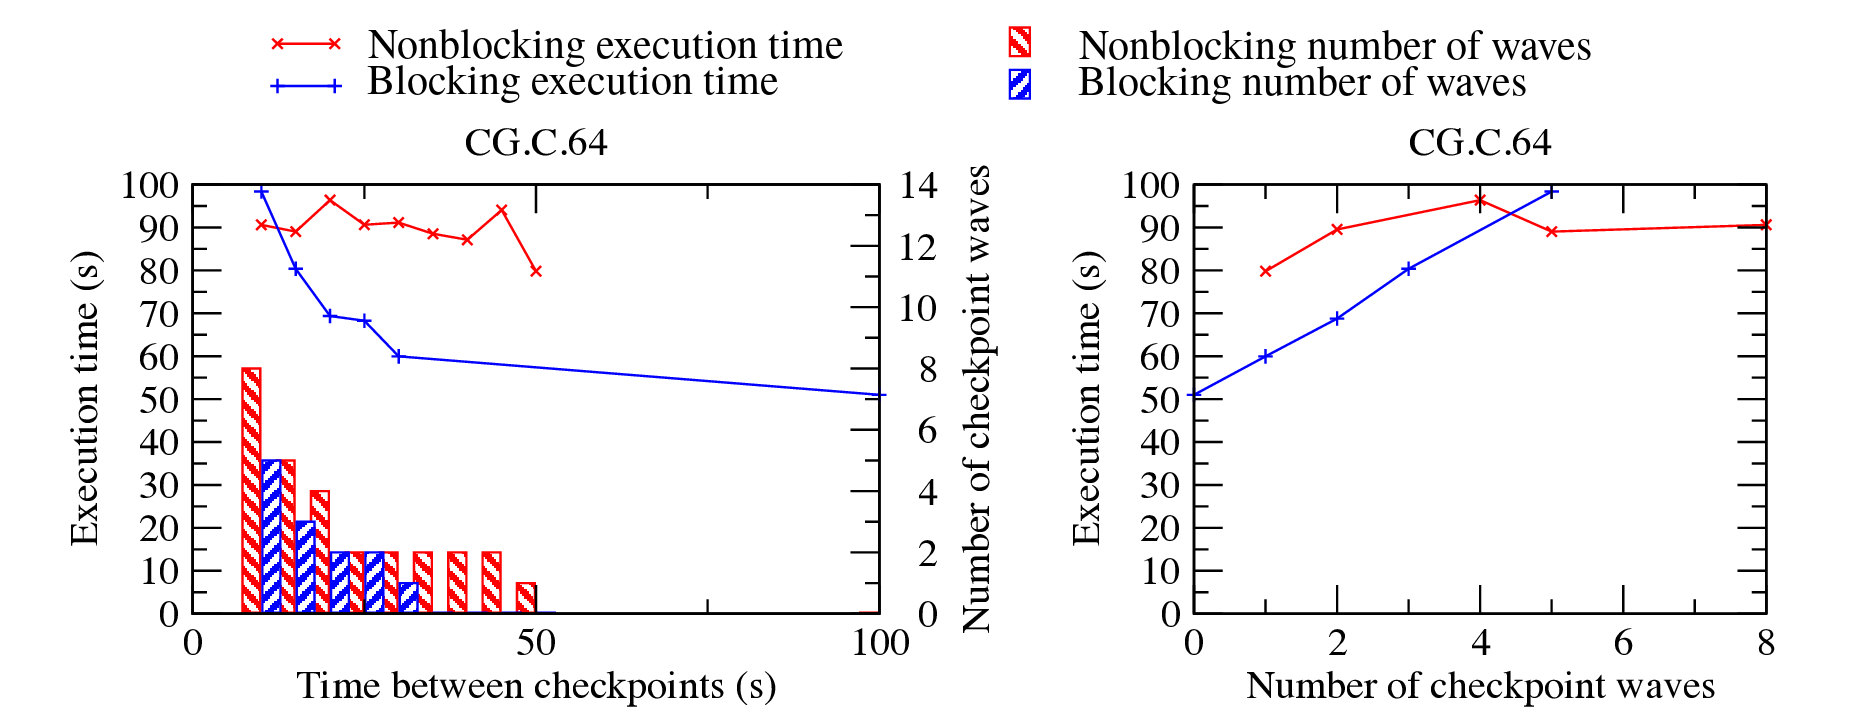
\includegraphics[width=\linewidth]{figures/mpichv-coordinated.png}\\
        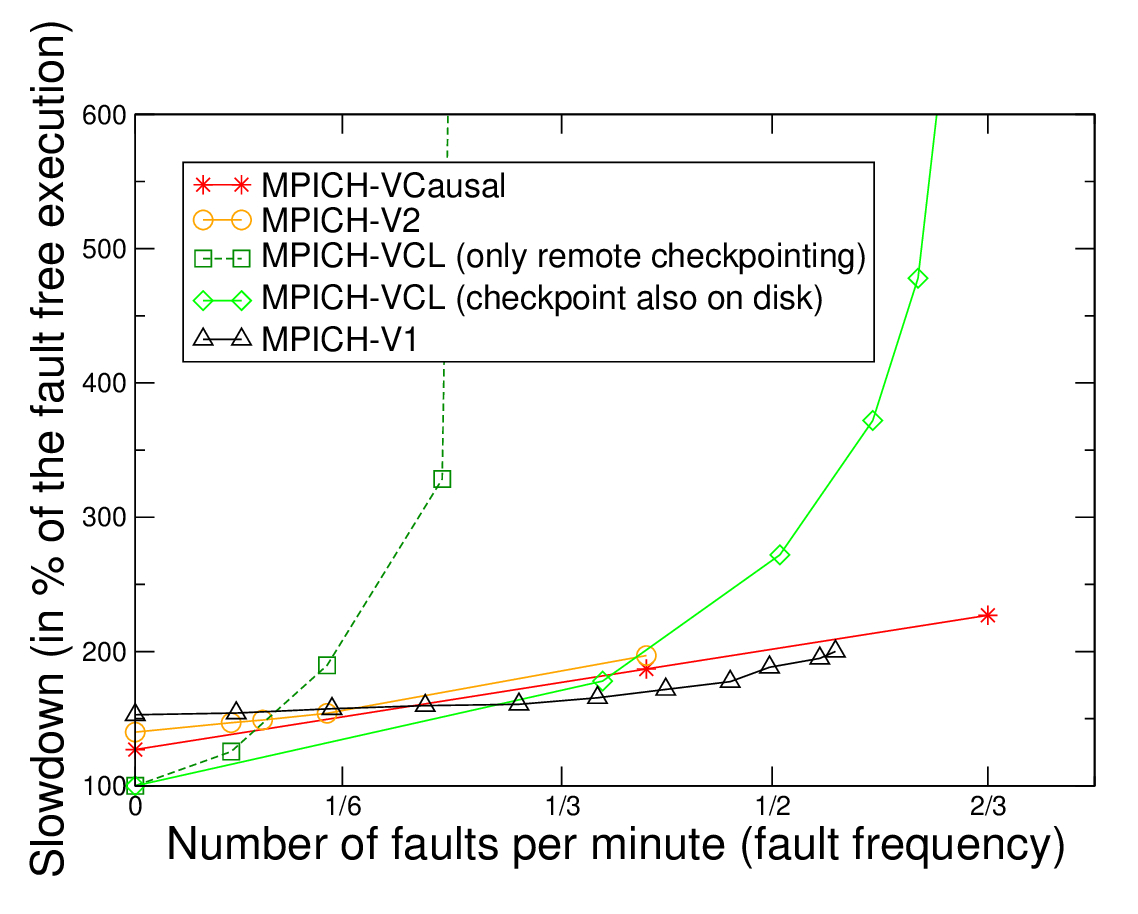
\includegraphics[width=.75\linewidth]{figures/mpichv-noncoordinated.jpg}
      \end{center}
    \end{column}
    \begin{column}{.45\linewidth}
      \begin{itemize}
      \item MPICH-V: studied experimentally rollback-recovery protocols in a Message Passing Interface library (MPICH)
      \item Subject: how to checkpoint efficiently
        \begin{itemize}
        \item Coordinated protocols (blocking, non-blocking)
        \item Uncoordinated protocols (Optimistic, Pessimistic, Causal)
        \end{itemize}
      \item Uncovered: when to checkpoint
      \end{itemize}
    \end{column}
  \end{columns}  
}

\begin{frame}
  \frametitle{Periodic checkpointing}

\begin{center}
  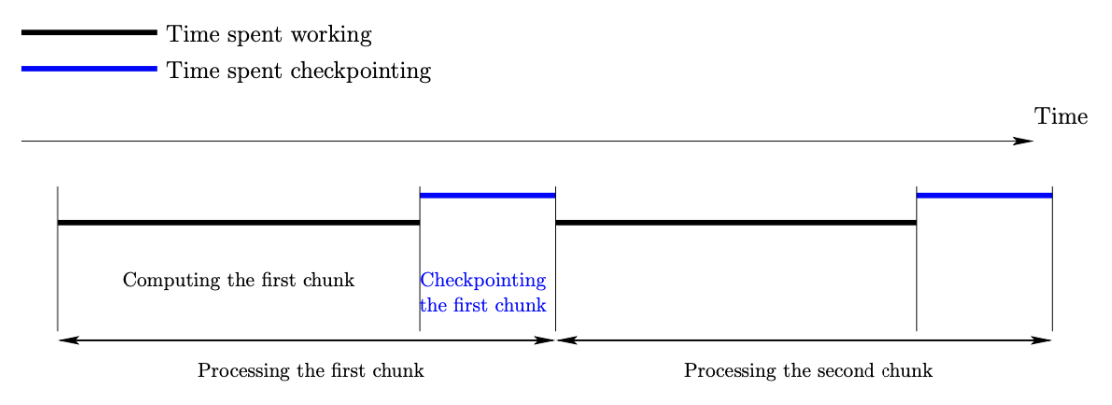
\includegraphics[width=.9\textwidth]{PeriodicCoordinatedCkpt.png}%
 \end{center}

\textbf{Blocking model:} while a checkpoint is taken, no computation can be performed
  
\end{frame}

\begin{frame}
  \frametitle{Waste in failure-free execution}

\vfill
\centering
\begin{tabular}{cc}
\begin{minipage}{.55\textwidth}
 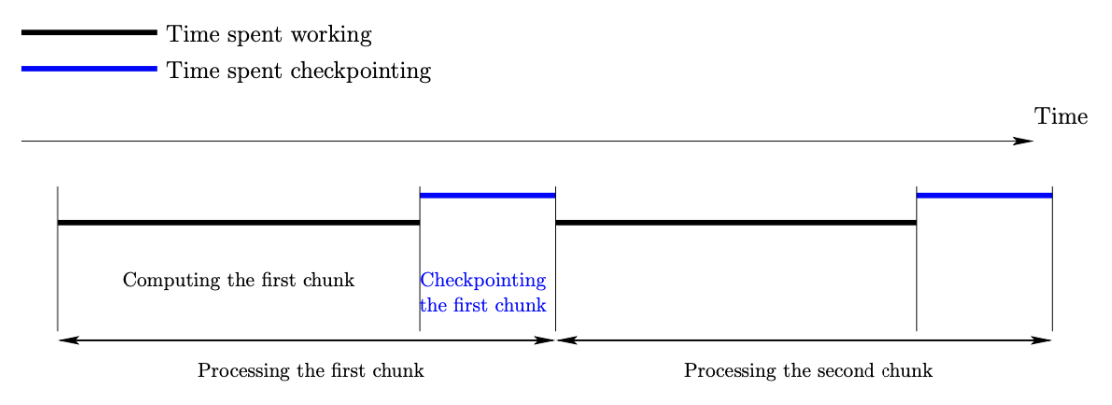
\includegraphics[width=\textwidth]{PeriodicCoordinatedCkpt.png}
\end{minipage}
&
\begin{minipage}{.65\textwidth}
\begin{itemize}
      \item  \Time[base]: application base time
       \item \Time[FF]: with periodic checkpoints\\
       but failure-free
 \end{itemize}
 \end{minipage}
 \end{tabular}
 
$$\Time[FF]  =  \Time[base] + \#checkpoints \times \Cr$$
$$\#checkpoints  = 
\left\lceil\frac{\Time[base]}{\period-\Cr}\right\rceil
\sim \frac{\Time[base] }{\period-\Cr} \text{ (valid for large jobs)}$$

\red{$$\Waste[FF] = \frac{\Time[FF]-\Time[base]}{\Time[FF]} = \frac{\Cr}{\period}$$}

\end{frame}

\begin{frame}
    \frametitle{Waste due to failures}
    
\begin{center}
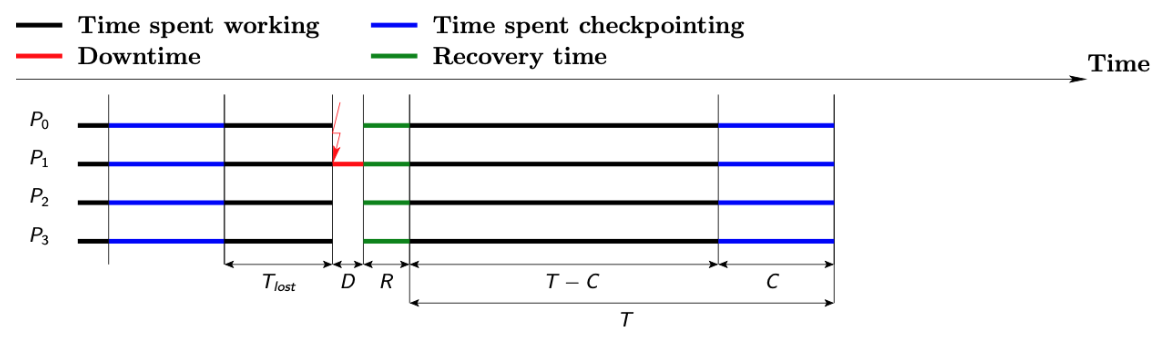
\includegraphics[width=0.95\textwidth]{NewYvesCoordinated.png}
\end{center}
$$\Tlost= \D+\R+ \frac{\period}{2}$$
  
\red{$$\Waste[fail] = \frac{1}{\mu} \left( \D + \R + \frac{\period}{2} \right)$$}


\end{frame}

\begin{frame}
  \frametitle{Total waste}
 
\centering
\centering
\begin{tikztimingtable}[
    timing/slope=0,         % no slope
    timing/rowdist=\ttrd,     % row distance
    timing/coldist=2pt,     % column distance
    xscale=3,yscale=1.5, % scale diagrams
    semithick ,              % set line width
  ]

 & G1.2D{\T-\C}G{[fill=black!20] 0.2D{\C}G}1.2D{\T-\C}G{[fill=black!20] 0.2D{\C}G}1.2D{\T-\C}G{[fill=black!20] 0.2D{\C}G}1.2D{\T-\C}G{[fill=black!20] 0.2D{\C}G}1.2D{\T-\C}G{[fill=black!20] 0.2D{\C}G}{[fill=black!80] 3DG}\\
\extracode
%  \tableheader{Probability}{\waste}
 \makeatletter
 \begin{pgfonlayer}{background}
%Ligne 0
%\arrowtime{0}{9.5};
\legende{0,0}{7}{\Time[FF]=\Time[Final](1-\Waste[Fail])};
%\legende{3.2,0}{0.9}{\Wregular};
%\legende{4.6,0}{1.1}{\T-\Wregular-\C};
\legende{7,0}{3}{$\Time[Final]\times\Waste[Fail]$};
\legende{0,-1.6}{10}{\Time[Final]};
 \end{pgfonlayer}
\end{tikztimingtable}%



$$\Waste= \frac{\Time[final]-\Time[base]}{\Time[final]}$$
$$1 - \Waste = (1-\Waste[FF])(1-\Waste[fail])$$

\red{$$\Waste = \frac{\Cr}{\period} + \left( 1 -  \frac{\Cr}{\period} \right) 
	\frac{1}{\mu} \left( \D + \R + \frac{\period}{2} \right)$$}
\end{frame}

\begin{frame}
  \frametitle{Waste minimization}
 

$$\Waste = \frac{\Cr}{\period} + \left( 1 -  \frac{\Cr}{\period} \right) 
	\frac{1}{\mu} \left( \D + \R + \frac{\period}{2} \right)$$


$$\Waste =  \frac{u}{\period} + v + w \period$$
$$u=\Cr \big( 1 - \frac{\D+\R}{\mu} \big) \qquad v =  \frac{\D+\R- \Cr/2}{\mu} \qquad w= \frac{1}{2\mu}$$


\vfill
\noindent
$\Waste$  minimized for $\period = \sqrt{\frac{u}{w}}$


\red{$$\T = \sqrt{2(\mu - (\D+\R)) \Cr}$$}

\end{frame}

\begin{frame}
\frametitle{Optimal checkpointing interval}

\begin{columns}
  \begin{column}{.6\linewidth}
    \begin{center}
      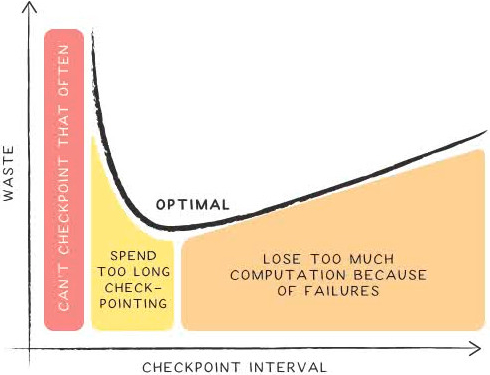
\includegraphics[width=\columnwidth]{resilience}
    \end{center}
  \end{column}
  \begin{column}{.4\linewidth}
    \small
    \textbf{First-order approximation [Young,Daly]:}\\
    Optimal period length:
    $$\blue{W^{\opt}} = \blue{\sqrt{2\mu C}}$$\\
    Corresponding overhead:
    $$\blue{H_{\text{opt}}} = \blue{\sqrt{\frac{2C}{\mu}}}$$
  \end{column}
\end{columns}

\end{frame}

\begin{frame}
  \frametitle{Hierarchical checkpointing}
  
\centerline{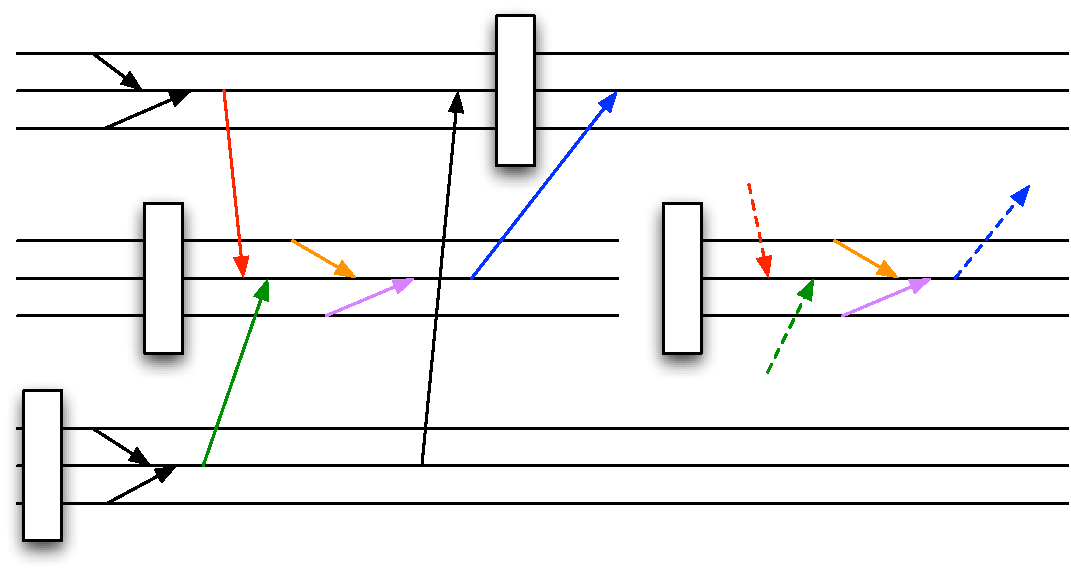
\includegraphics[width=.5\textwidth]{HierarFull.pdf}}

\vfill
  
\only<1>{\begin{itemize}
\item Non-coordinated protocols with Message Logging:
  \begin{itemize}
  \item Checkpoints are not coordinated
  \item Messages (and other nondeterministic events) are logged and replayed
  \end{itemize}
\item Hierarchical Protocols:
  \begin{itemize}
  \item Processors partitioned into $G$ groups of $q$ processors each
  \item Coordinated checkpointing inside each group, noncoordinated between groups
  \end{itemize}
\end{itemize}}
\only<2>{
  \begin{itemize}
  \item How to group processes:
    \begin{itemize}
    \item Per physical resources (high probability of simultaneous failure)
    \item Per communication group (high frequency of intra-group messages)
    \end{itemize}
  \item Expected advantages:
    \begin{itemize}
    \item[\smiley] no synchronization overheads 
    \item[\smiley] checkpoints are staggered
    \item[\smiley] only failed processes need to restart
    \end{itemize}
  \end{itemize}
}

\end{frame}

\begin{frame}
  \frametitle{Hierarchical Checkpointing: Failure during computing phase}

  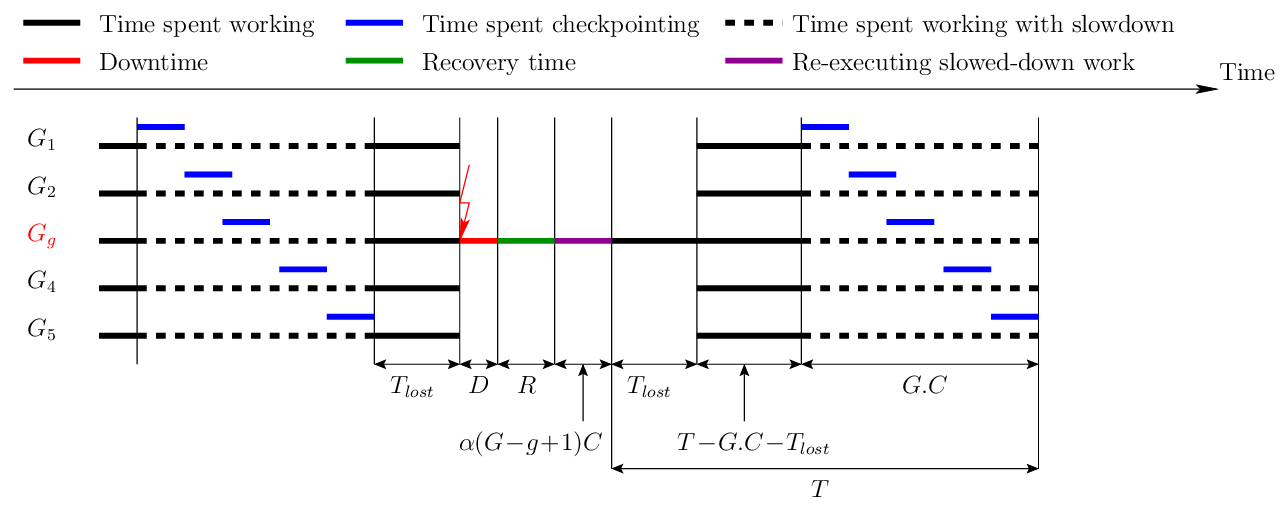
\includegraphics{hierarchical_failure_comp.png}

  \Overhead: $T_{lost}+\alpha(G-g+1)C$\\
  Expectation: $T_{lost}= \frac{1}{2}(T-G.C)$\\
  Approximated \Overhead: $\frac{T-G.C}{2}+\alpha(G-g+1)C$
  
\end{frame}

\begin{frame}
  \frametitle{Failure during checkpoint phase: Failure before checkpoint}

  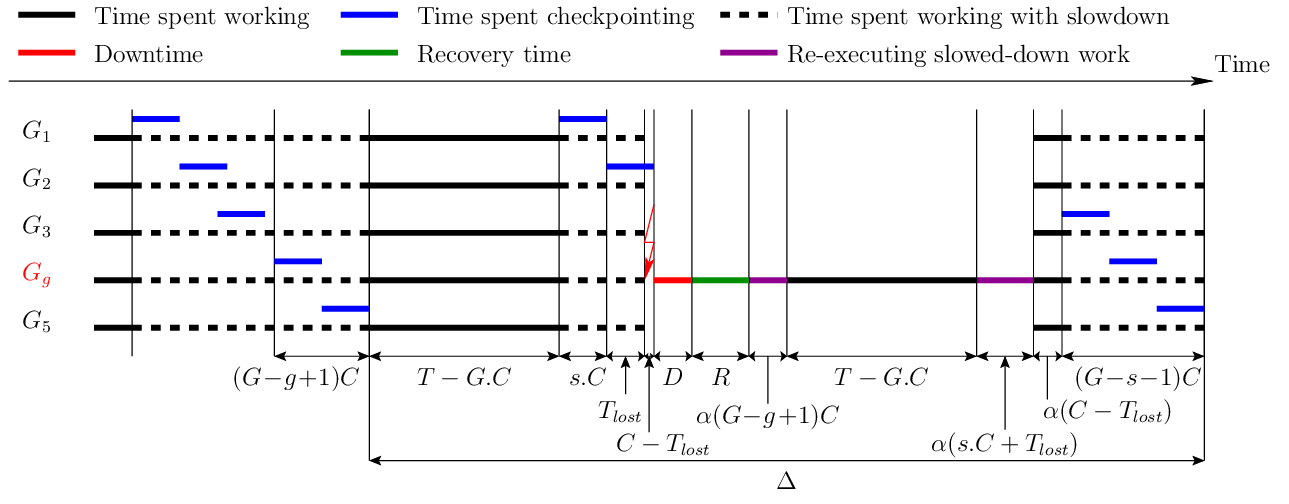
\includegraphics{hierarchical_failure_before_ckpt.png}

  Average \Overhead~for group $g$ (for $2 \leq g \leq G$):
    \begin{multline*}
      \frac{1}{g-1}\sum_{s=0}^{g-2} \left(T +
        ((\alpha-1)G+\alpha(-g+s+2)).C(q)\right) + D(q) + R(q)\\
      = T + D(q)+R(q)+\left((\alpha-1)G-\alpha\frac{g-2}{2}\right).C(q)
    \end{multline*}
  
\end{frame}

\begin{frame}
  \frametitle{Failure during checkpoint phase: Failure during checkpoint}

  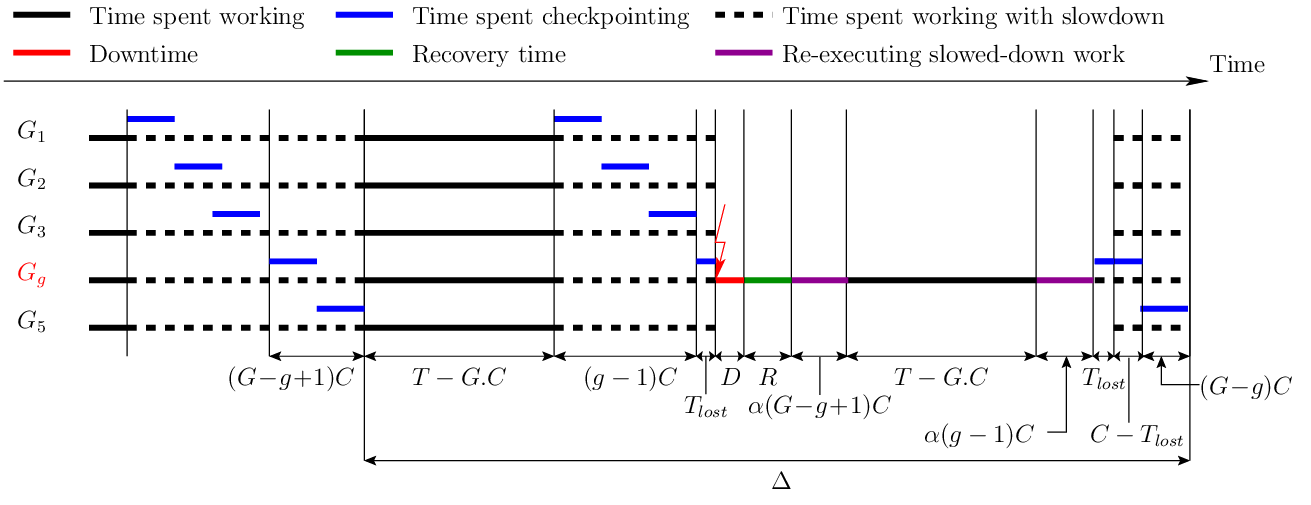
\includegraphics{hierarchical_failure_during_ckpt.png}

  \Overhead = $T+(\alpha-1)G.C + T_{lost}$
  
  Expectation: $T_{lost} = \frac{C}{2}$

  Approximated \Overhead  $$T+(\alpha-1)G.C(q)+\frac{C(q)}{2}$$
  
\end{frame}

\begin{frame}
  \frametitle{Failure during checkpoint phase: Failure after checkpoint}

  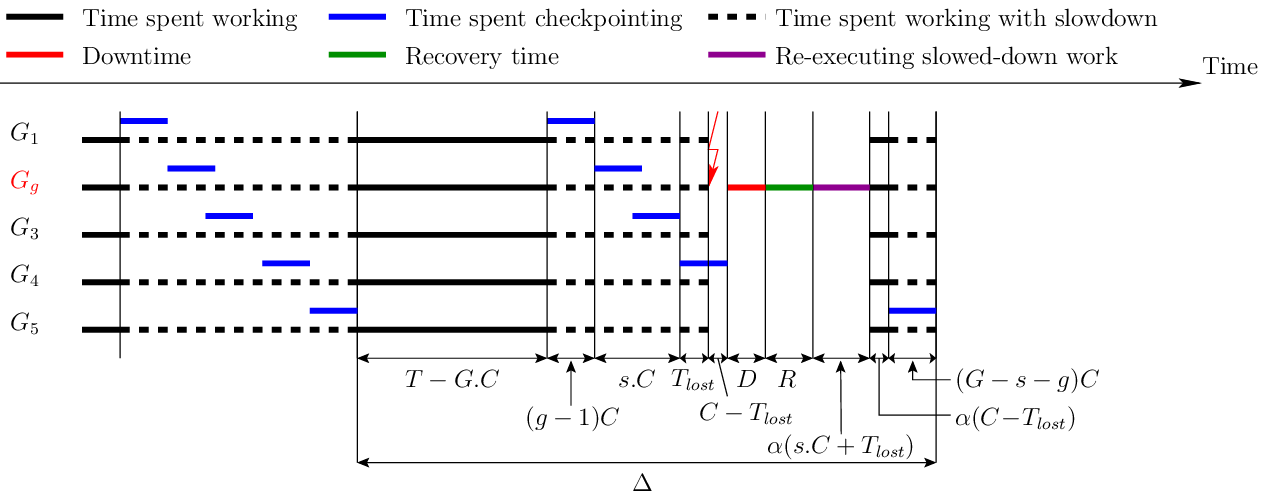
\includegraphics{hierarchical_failure_after_ckpt.png}

  \Overhead = $ \alpha(s+1)C$

  Average \Overhead~for group $g$ (for $1 \leq g \leq G-1$): 
  \begin{multline*}
    \frac{1}{G-g}\sum_{s=1}^{G-g}\left(\alpha(s+1)C(q)\right)= \alpha\frac{G-g+3}{2}C(q)
  \end{multline*}
  
\end{frame}

\begin{frame}
  \frametitle{Average waste for failures during checkpointing
    phase}
  
  Average \Overhead\ when the failing-group $g$ fails

  Overall average \Overhead: $\ockpt = $\\[-5mm]
  \begin{multline*}
    \frac{1}{G} ( (g\!-\!1) . \obckpt +
      1.  \odckpt\\ + (G\!-\!g) . \oackpt)
  \end{multline*}
  \vfill
    Average over all groups:
    \begin{multline*}
      \avgockpt =\\ \frac{G+1}{2G}T + \frac{\alpha
        C(q)(G+3)}{2}+\frac{C(q)(1-2\alpha)}{2G} -\frac{C(q)(G+1)}{2}
    \end{multline*}
\end{frame}

\begin{frame}
  \frametitle{Total waste}
  
  $$
  \begin{array}{l}
    \displaystyle \Waste[FF] =  \frac{T-\Work}{T} \text{ with } \Work = T - (1-\alpha) G C(q)\\
    \displaystyle \Waste[fail] = \frac{1}{\muplatform} \bigg( \dgroup + \rgroup + \Overhead \bigg) \text{ with } \\[3mm]
    \displaystyle \Overhead =   \frac{\T\!-\!\ngroups\cgroup}{\T} \ocomp +  \frac{\ngroups\cgroup}{\T} \ockpt \\[5mm]
      \displaystyle \Waste = \Waste[FF] + \Waste[fail] - \Waste[FF] \Waste[fail]
 \end{array}
 $$ 
\end{frame}

\begin{frame}
  \frametitle{Accounting for message logging: Impact on work}

 \begin{itemize}
  \item \frownie Logging messages slows down execution:\\
  $\Rightarrow$ $\Work$ becomes $\red{\lambda} \Work$, where $0 < \lambda <1$\\
  Typical value: $ \lambda \sim 0.98$

  \item \smiley Re-execution after a failure is faster:\\
  $\Rightarrow$ $\Overhead$ becomes $\frac{\Overhead}{\red{\rho}}$, where $\rho \in[1..2]$\\
   Typical value: $ \rho \sim 1.5$
  
  \end{itemize}

\vfill
$$\Waste[FF] = \frac{\T - \red{\lambda} \Work}{\T}$$
$$\Waste[fail] = \frac{1}{\muplatform} \bigg( \dgroup + \rgroup + 
\frac{\Overhead}{\red{\rho}} \bigg) $$
\end{frame}


\begin{frame}
  \frametitle{Accounting for message logging: Impact on checkpoint size}

 \begin{itemize}
 \item Inter-groups messages logged continuously
 \item  Checkpoint size increases with amount of work executed before a checkpoint
 \item $\cgroupbase$: Checkpoint size of a group without message logging
$$
\cgroup = \cgroupbase (1 + \amountlog \Work) \Leftrightarrow \color{red}{\amountlog = \frac{\cgroup - \cgroupbase}{\cgroupbase \Work}}
$$
%\begin{overlayarea}{\linewidth}{2cm}{
$$\Work = \lambda (\T - (1-\workduringckpt)\ngroups\cgroup)$$
$$\cgroup = \frac{ \cgroupbase (1 + \amountlog \lambda \T)}{1+ \ngroups \cgroupbase \amountlog \lambda (1-\workduringckpt)}$$

%\end{overlayarea}
%% \item
%% Constraint $ \ngroups \cgroup \leq \T$ translates into 
%% $$
%% \ngroups \cgroupbase \amountlog \lambda \workduringckpt \leq 1 \text{ and } \T \geq \frac{\ngroups \cgroupbase }{1- \ngroups \cgroupbase \amountlog \lambda \workduringckpt} $$

 \end{itemize}

 \vfill
 Minimize $\Waste$ subject to:
  \begin{itemize}
  \item $G C(q) \leq T$ (by construction)
  \item Gets complicated! Use computer algebra software \frownie
  \end{itemize}
\end{frame}

\begin{frame}
  \frametitle{Platforms: basic characteristics}
  
  \begin{center}\sffamily\scriptsize
    \resizebox{0.9\linewidth}{!}
    %\scalebox{0.85}
    {\hspace*{-1cm} \begin{tabular}{|c|c|c|c|c|c|c|c|}\hline
        Name 			& Number of     & Number of 			& Number of cores	& Memory  		& \multicolumn{2}{c|}{I/O Network Bandwidth (\bwio)} 	& I/O Bandwidth (\bwnode)\\
        &  cores     	& processors \nprocess  & per processor     & per processor & Read 		& Write 									& Read/Write per processor \\\hline
        Titan  			& 299,008       & 16,688  				& 16                & 32GB 			& 300GB/s 	& 300GB/s 									& 20GB/s \\\hline
        Exascale-Slim 	& 1,000,000,000 & 1,000,000 			& 1,000             & 64GB         	& 1TB/s     & 1TB/s     								& 200GB/s \\\hline
        Exascale-Fat	& 1,000,000,000 & 100,000 				& 10,000            & 640GB       	& 1TB/s     & 1TB/s     								& 400GB/s \\\hline
      \end{tabular}}
  \end{center}

\vfill

\begin{center}%\sffamily\scriptsize
\resizebox{0.7\linewidth}{!}
%\scalebox{0.85}
{\begin{tabular}{|c|c|c|c|c|c|c|}
\hline
Name 			& Scenario	& \ngroups (\cgroup) 	& \amountlog for  	& \amountlog for \\
          		&           & 					 	& \StenTwo 			&  \Matprod \\\hline
                                                    
          		& \CSCI     & 1 (2,048s) 			& / 				& /\\
Titan  			& \CSHI     & 136 (15s)   			& 0.0001098         & 0.0004280 \\ 
          		& \CSHP    	& 1,246 (1.6s) 			& 0.0002196  		& 0.0008561  \\\hline
                                        			                                        			
            	& \CSCI   	& 1 (1,000s/100s)		& / 				& /  \\
Exascale-Slim	& \CSHI 	& 1,000 (64s)   		& 0.0002599         & 0.001013      \\ 
         		& \CSHP 	& 200,0000 (0.32s) 		& 0.0005199  		& 0.002026   \\\hline
                                        			
         		& \CSCI   	& 1 (1,000s/100s)		& / 				& /  \\
Exascale-Fat	& \CSHI 	& 316 (217s)  			& 0.00008220        & 0.0003203 \\ 
         		& \CSHP 	& 33,3333 (1.92s)		& 0.00016440    	& 0.0006407 \\\hline
\end{tabular}}

$\alpha = 0.3$, $\lambda = 0.98$ and $\rho = 1.5$
\end{center}

\end{frame}


\begin{frame}
\frametitle{Waste for Titan}
\vfill
\begin{tabular}{p{.3\textwidth}p{.3\textwidth}p{.3\textwidth}}
Stencil 2D & Matrix product & Stencil 3D\\
   \hspace{1cm} 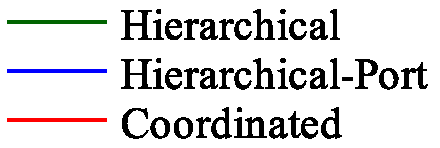
\includegraphics[width=0.3\linewidth]{3courbes.pdf} &
  \hspace{1.3cm} 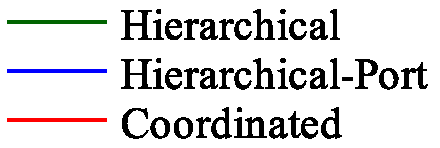
\includegraphics[width=0.3\linewidth]{3courbes.pdf}&
 \hspace{1.5cm}  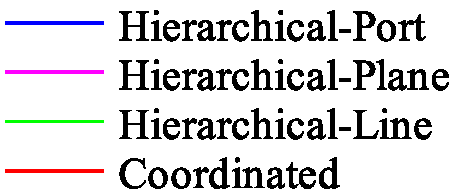
\includegraphics[width=0.2\linewidth]{4courbes.pdf} \\
  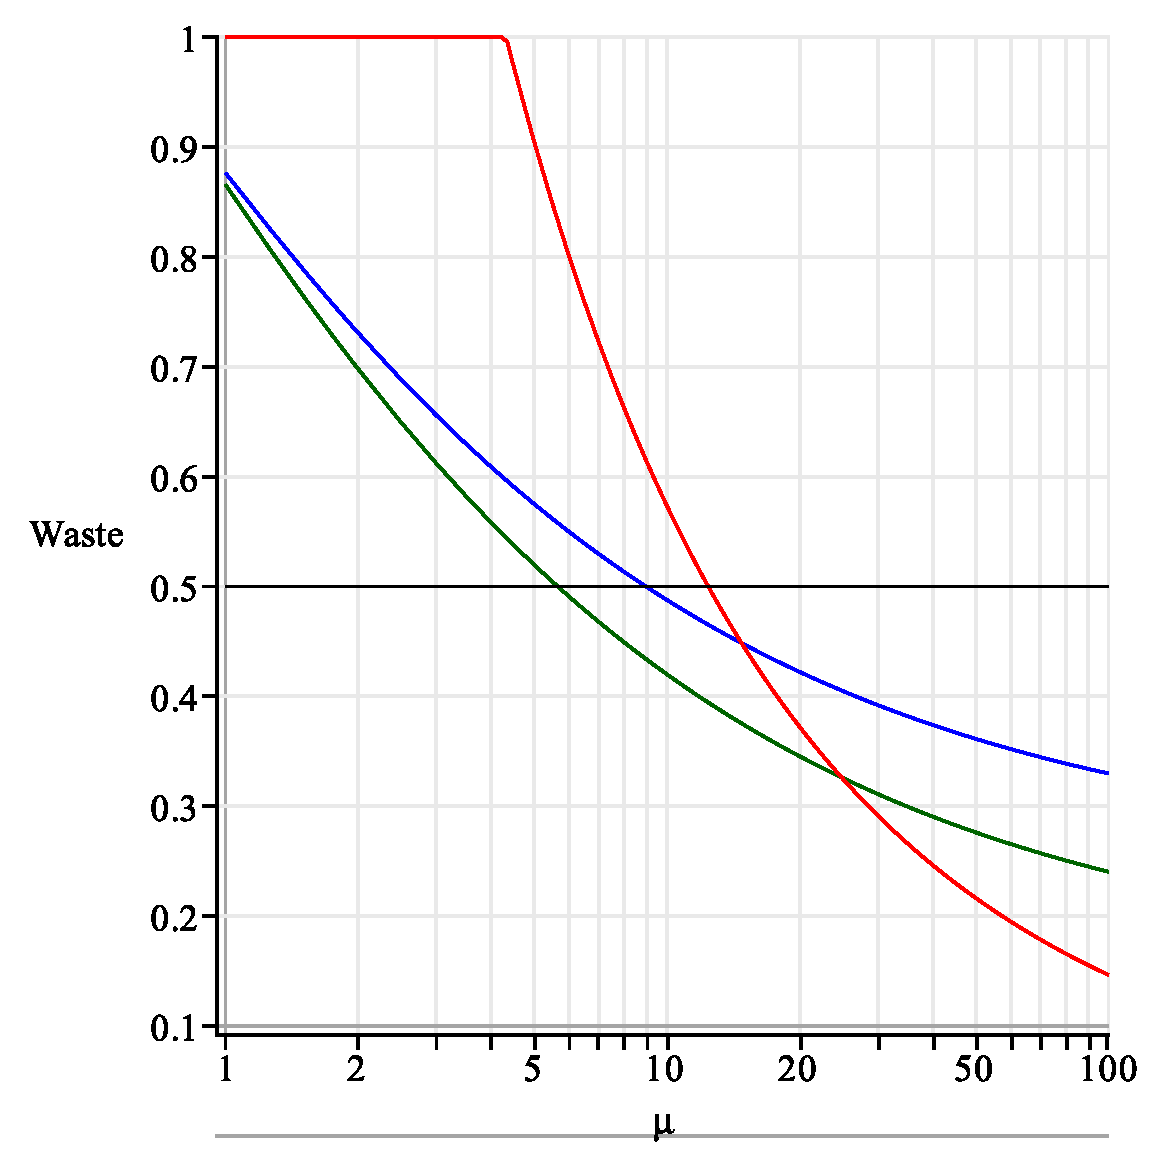
\includegraphics[width=0.3\textwidth,height=0.32\textheight,viewport=70 35 555 555,clip]{TitanWasteStenc.pdf} &
  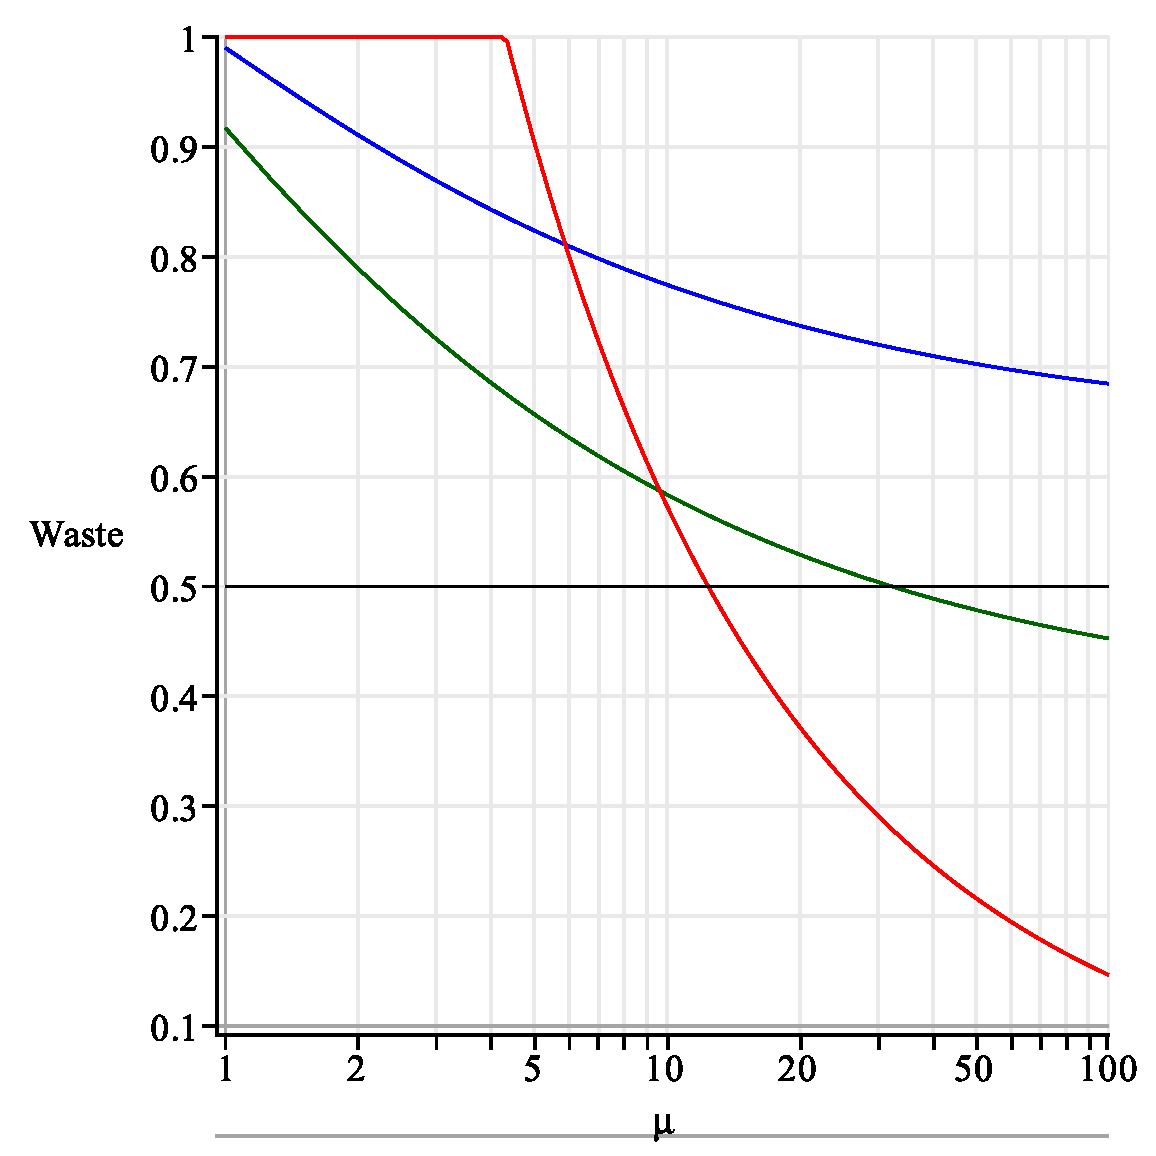
\includegraphics[width=0.3\textwidth,height=0.32\textheight,viewport=70 35 555 555,clip]{TitanWasteMat.pdf} &
  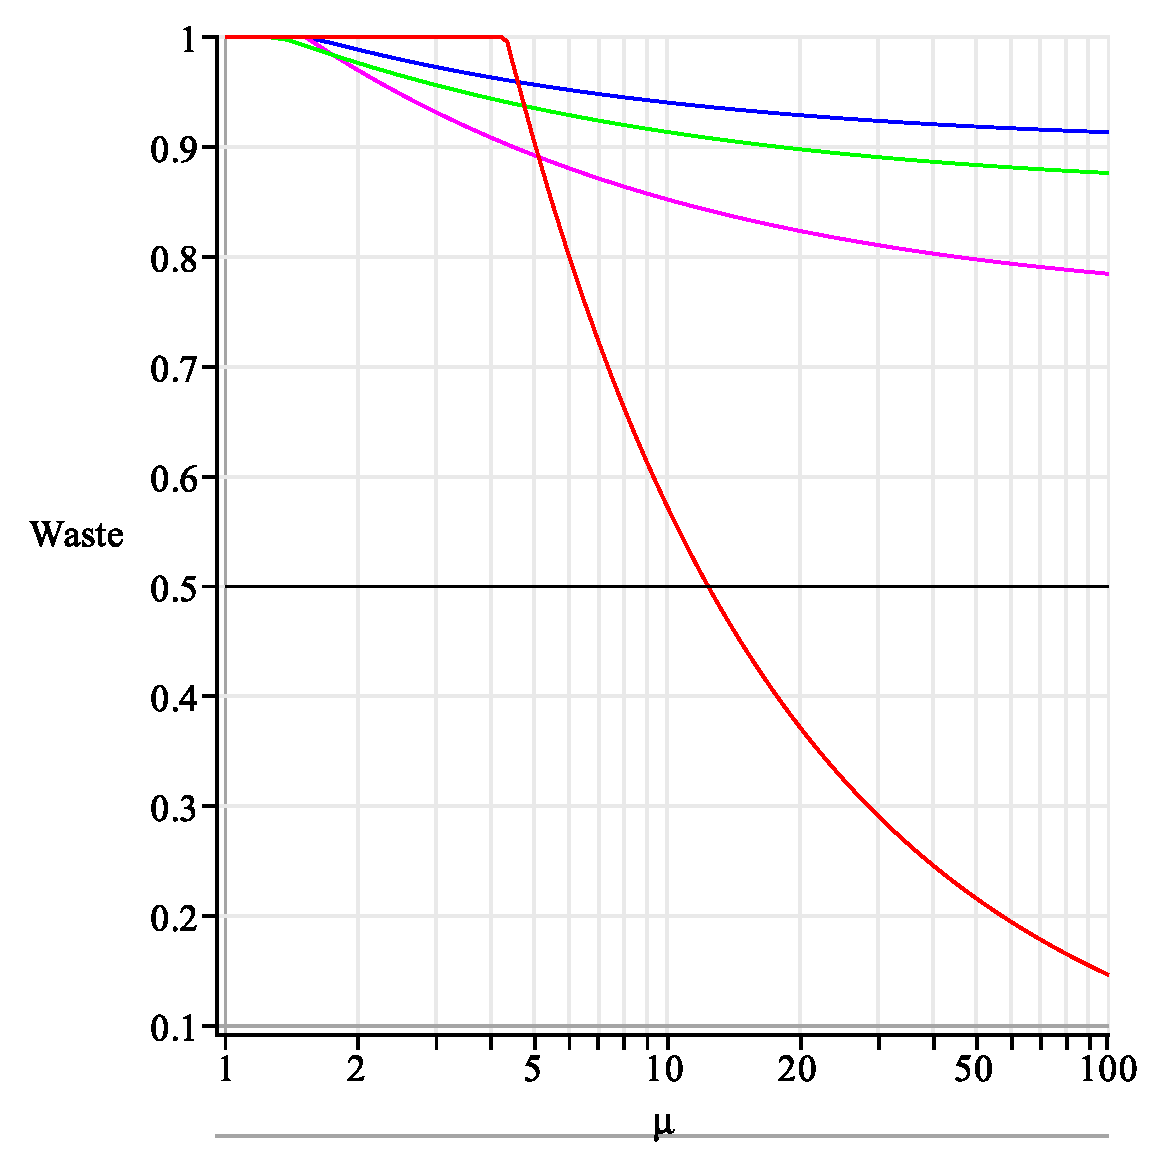
\includegraphics[width=0.3\textwidth,height=0.32\textheight,viewport=70 35 555 555,clip]{TitanWasteStenc3D.pdf} 
 \end{tabular}
 ~\\
\centerline{Waste as a function of processor MTBF $\mu_{ind}$}
\end{frame}


\begin{frame}
\frametitle{Waste for Prospective Exascale Platforms with $C=1,000$}
\vfill
\begin{tabular}{cp{.3\textwidth}p{.3\textwidth}p{.3\textwidth}}
& Stencil 2D & Matrix product & Stencil 3D\\
  & \hspace{1cm} 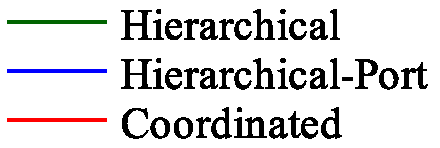
\includegraphics[width=0.3\linewidth]{3courbes.pdf} &
  \hspace{1.5cm} 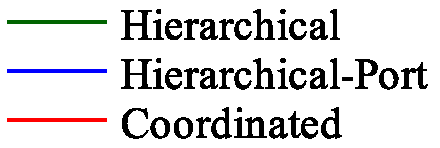
\includegraphics[width=0.3\linewidth]{3courbes.pdf}&
 \hspace{2cm}  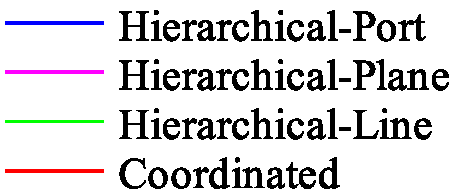
\includegraphics[width=0.2\linewidth]{4courbes.pdf} \\
 \rotatebox{90}{\hspace{.5cm}Exascale-Slim} &
  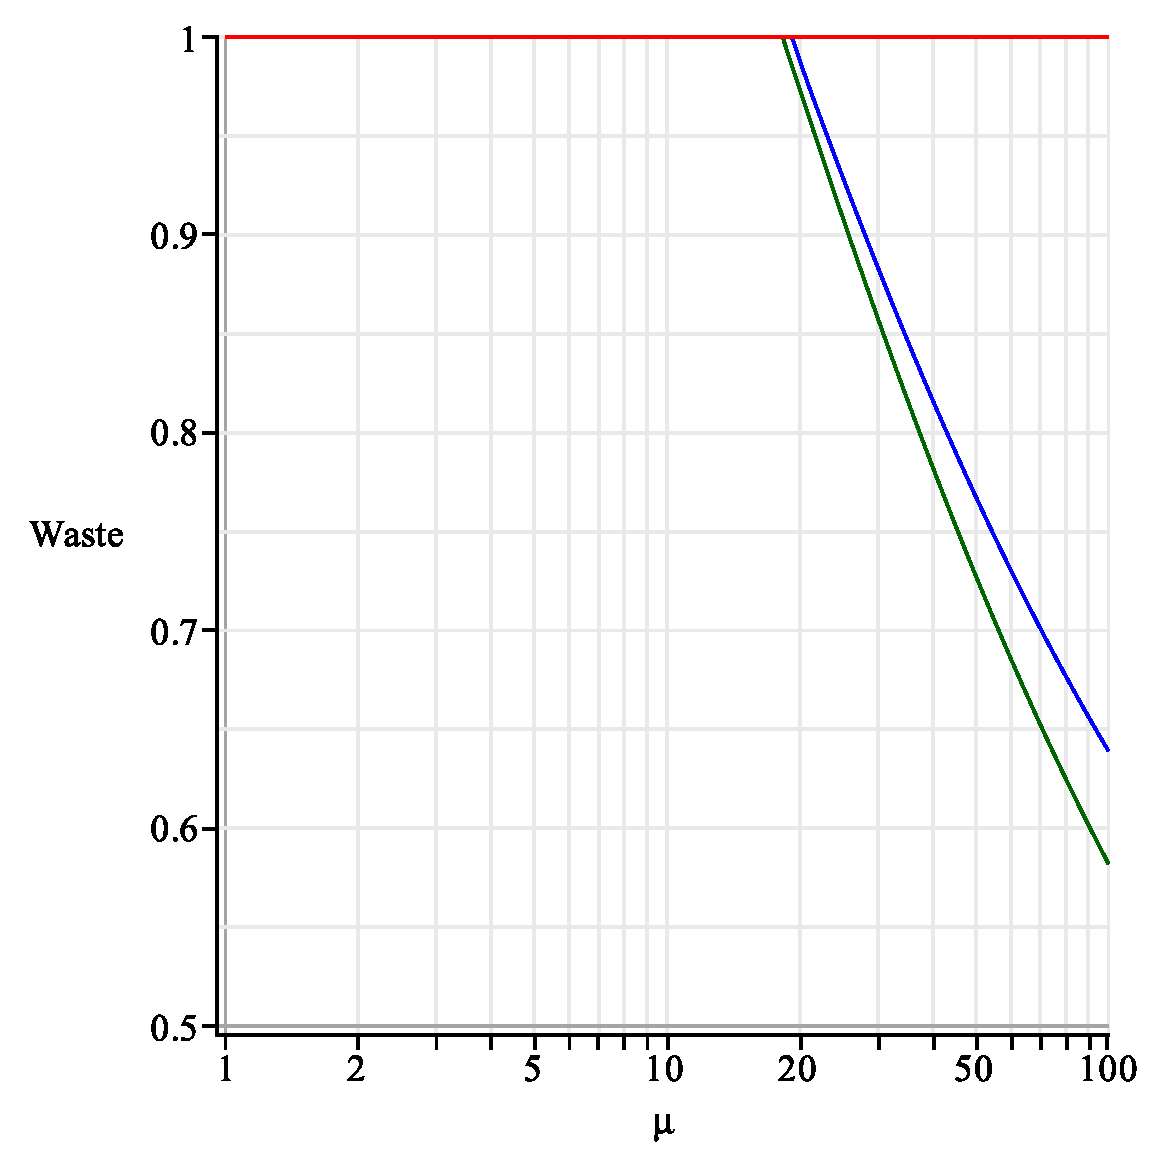
\includegraphics[width=0.3\textwidth,height=0.32\textheight,viewport=70 35 555 555,clip]{SlimWasteStenc1000.pdf} &
  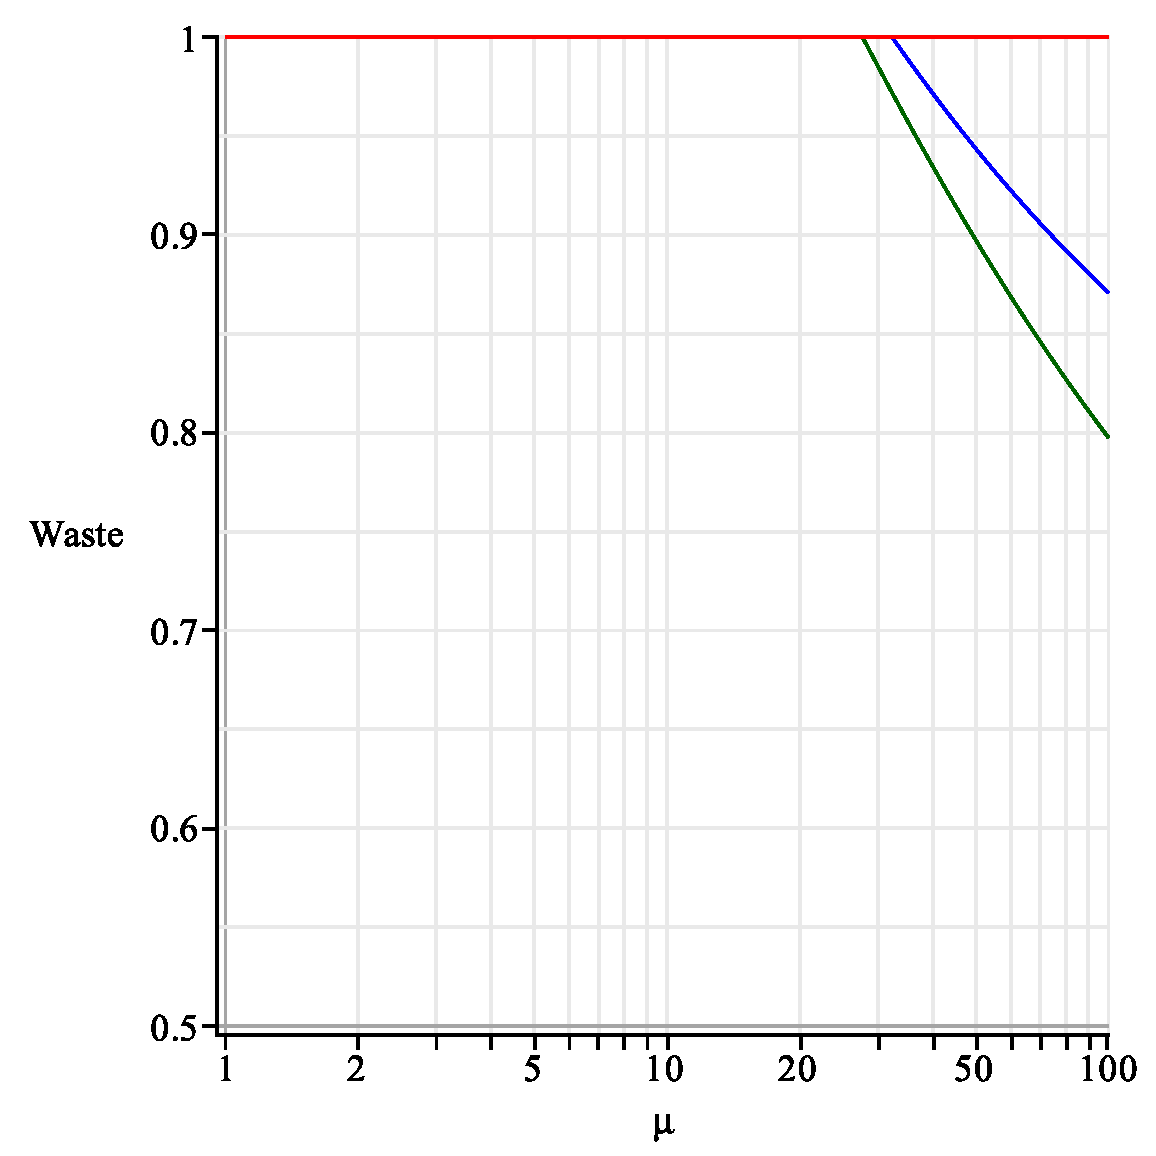
\includegraphics[width=0.3\textwidth,height=0.32\textheight,viewport=70 35 555 555,clip]{SlimWasteMat1000.pdf} &
  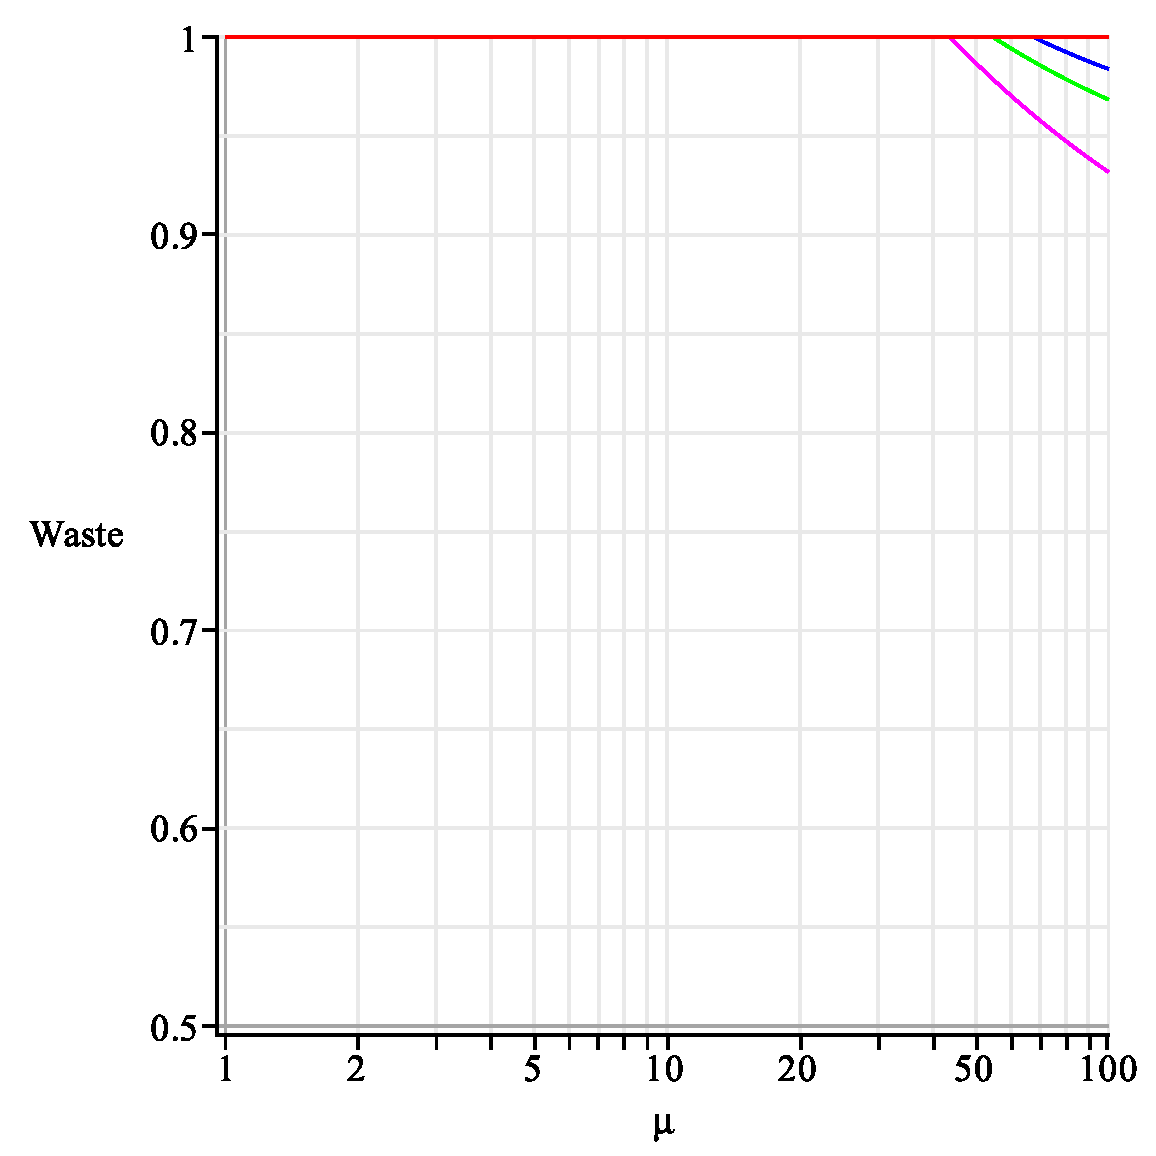
\includegraphics[width=0.3\textwidth,height=0.32\textheight,viewport=70 35 555 555,clip]{SlimWasteStenc3D1000.pdf} \\
   \rotatebox{90}{\hspace{.5cm}Exascale-Fat} &
    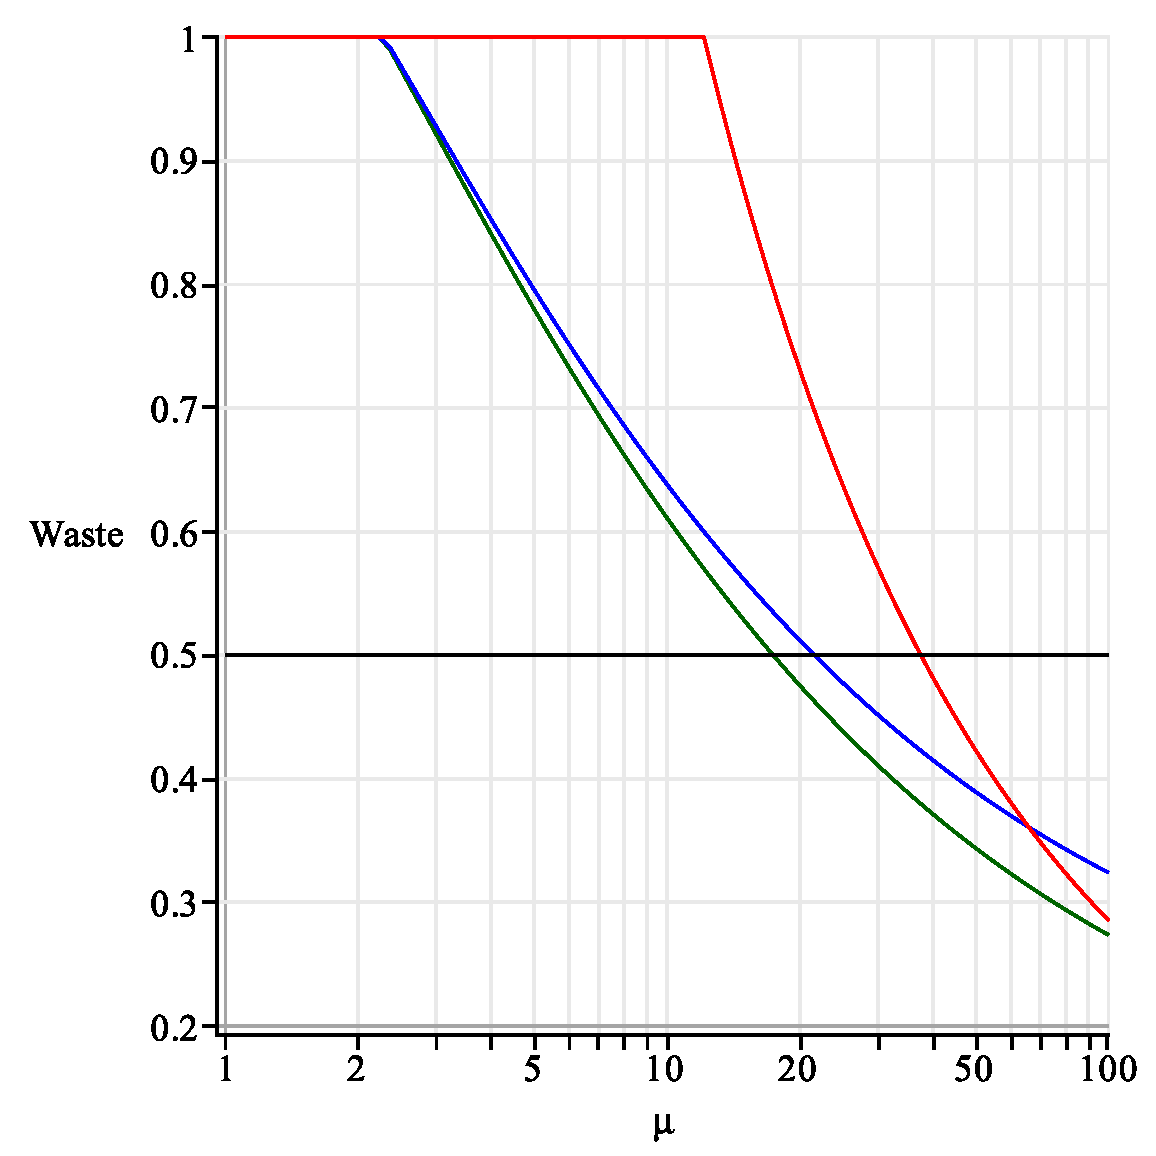
\includegraphics[width=0.3\textwidth,height=0.32\textheight,viewport=70 35 555 555,clip]{FatWasteStenc1000.pdf} &
  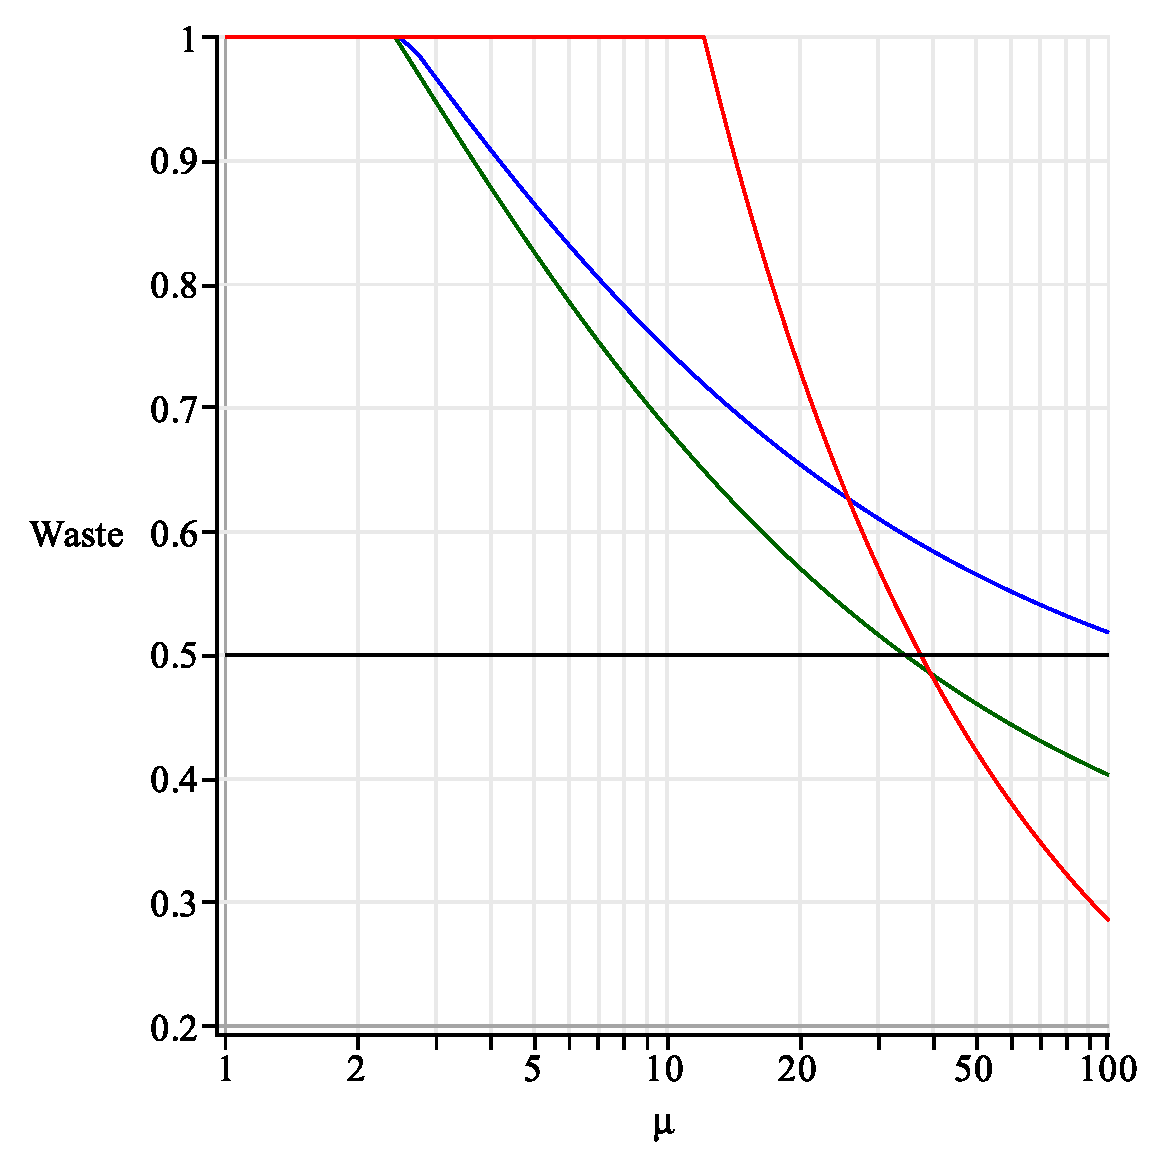
\includegraphics[width=0.3\textwidth,height=0.32\textheight,viewport=70 35 555 555,clip]{FatWasteMat1000.pdf} &
  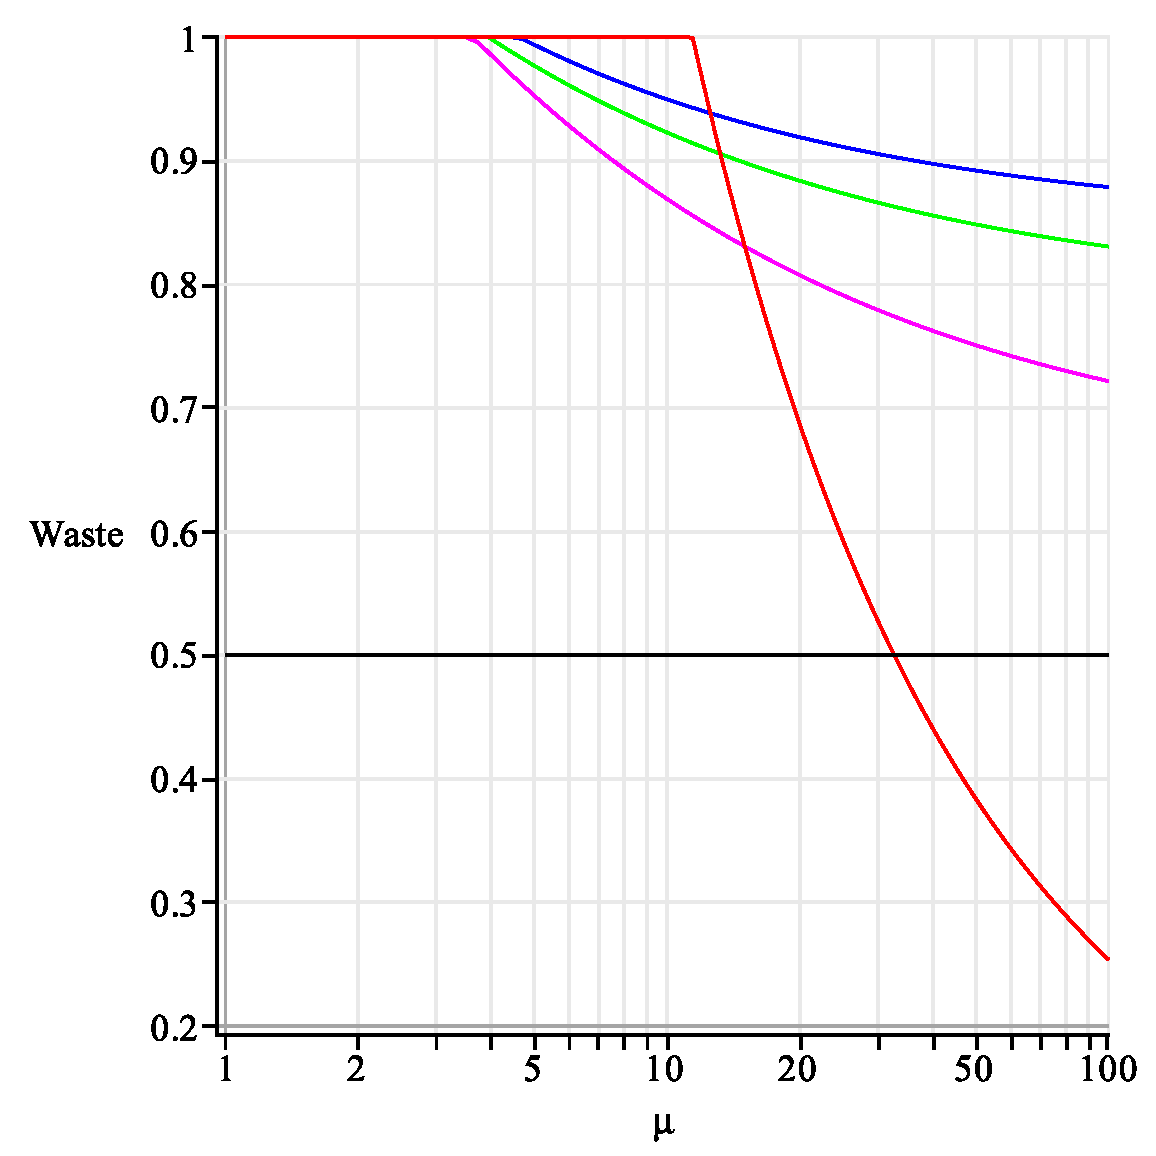
\includegraphics[width=0.3\textwidth,height=0.32\textheight,viewport=70 35 555 555,clip]{FatWasteStenc3D1000.pdf} \\
 \end{tabular}
 ~\\
\centerline{Waste as a function of processor MTBF $\mu_{ind}$, $C=1,000$}
\end{frame}

\begin{frame}
\frametitle{Waste for Prospective Exascale Platforms with $C=100$}
\vfill
\begin{tabular}{cp{.3\textwidth}p{.3\textwidth}p{.3\textwidth}}
& Stencil 2D & Matrix product & Stencil 3D\\
  & \hspace{1cm} 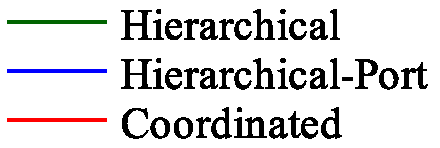
\includegraphics[width=0.3\linewidth]{3courbes.pdf} &
  \hspace{1.5cm} 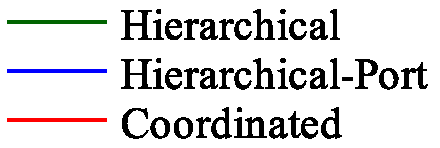
\includegraphics[width=0.3\linewidth]{3courbes.pdf}&
 \hspace{2cm}  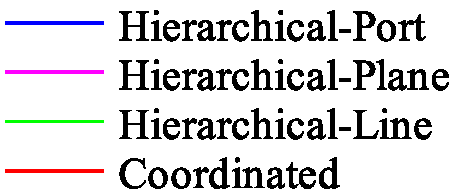
\includegraphics[width=0.2\linewidth]{4courbes.pdf} \\
 \rotatebox{90}{\hspace{.5cm}Exascale-Slim} &
  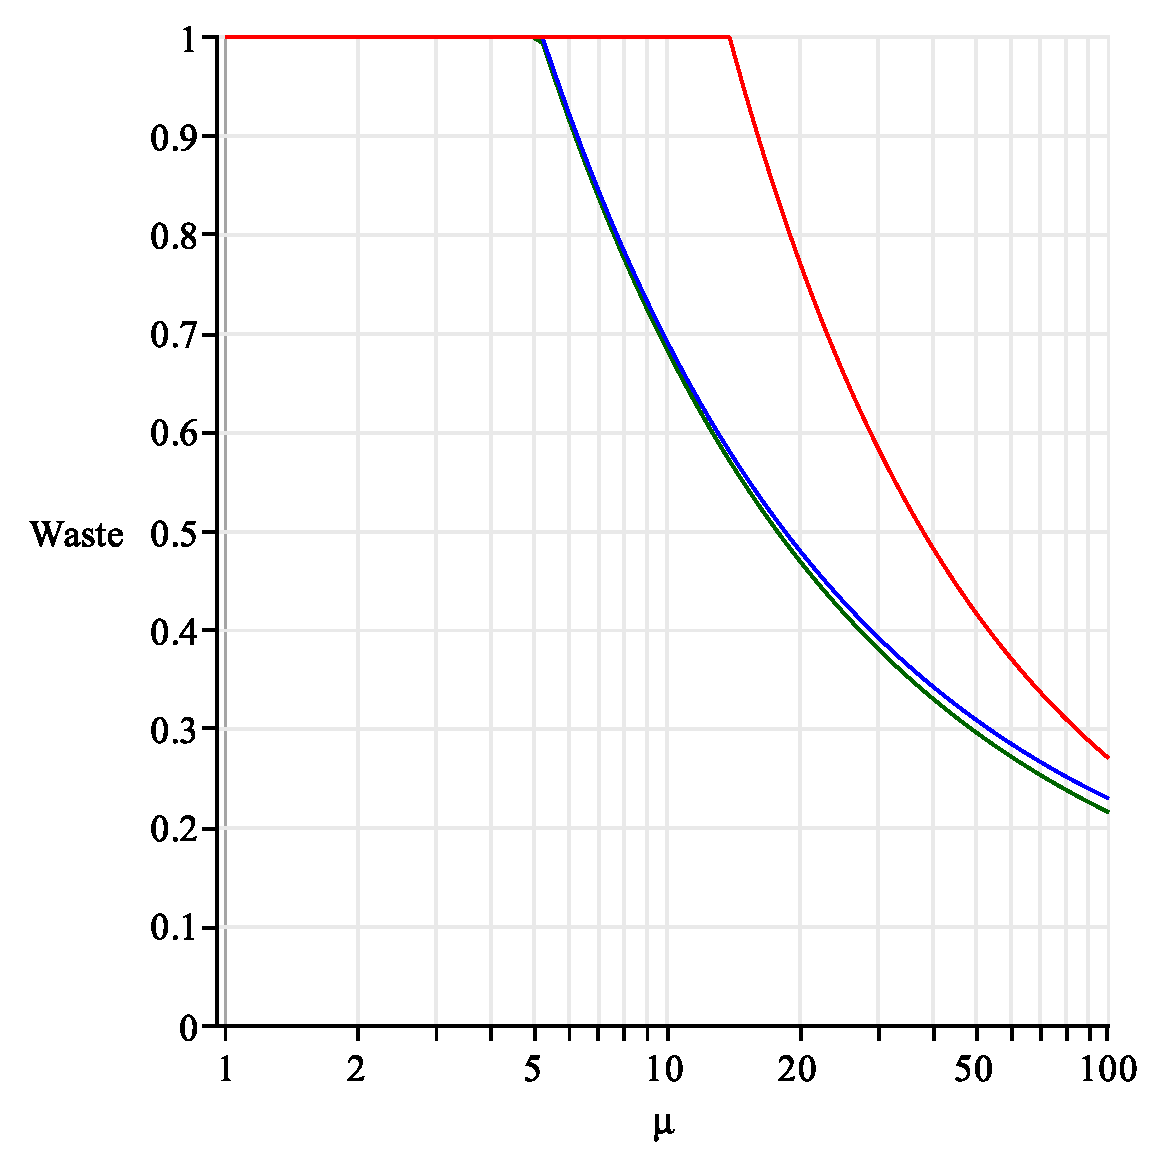
\includegraphics[width=0.3\textwidth,height=0.32\textheight,viewport=70 35 555 555,clip]{SlimWasteStenc100.pdf} &
  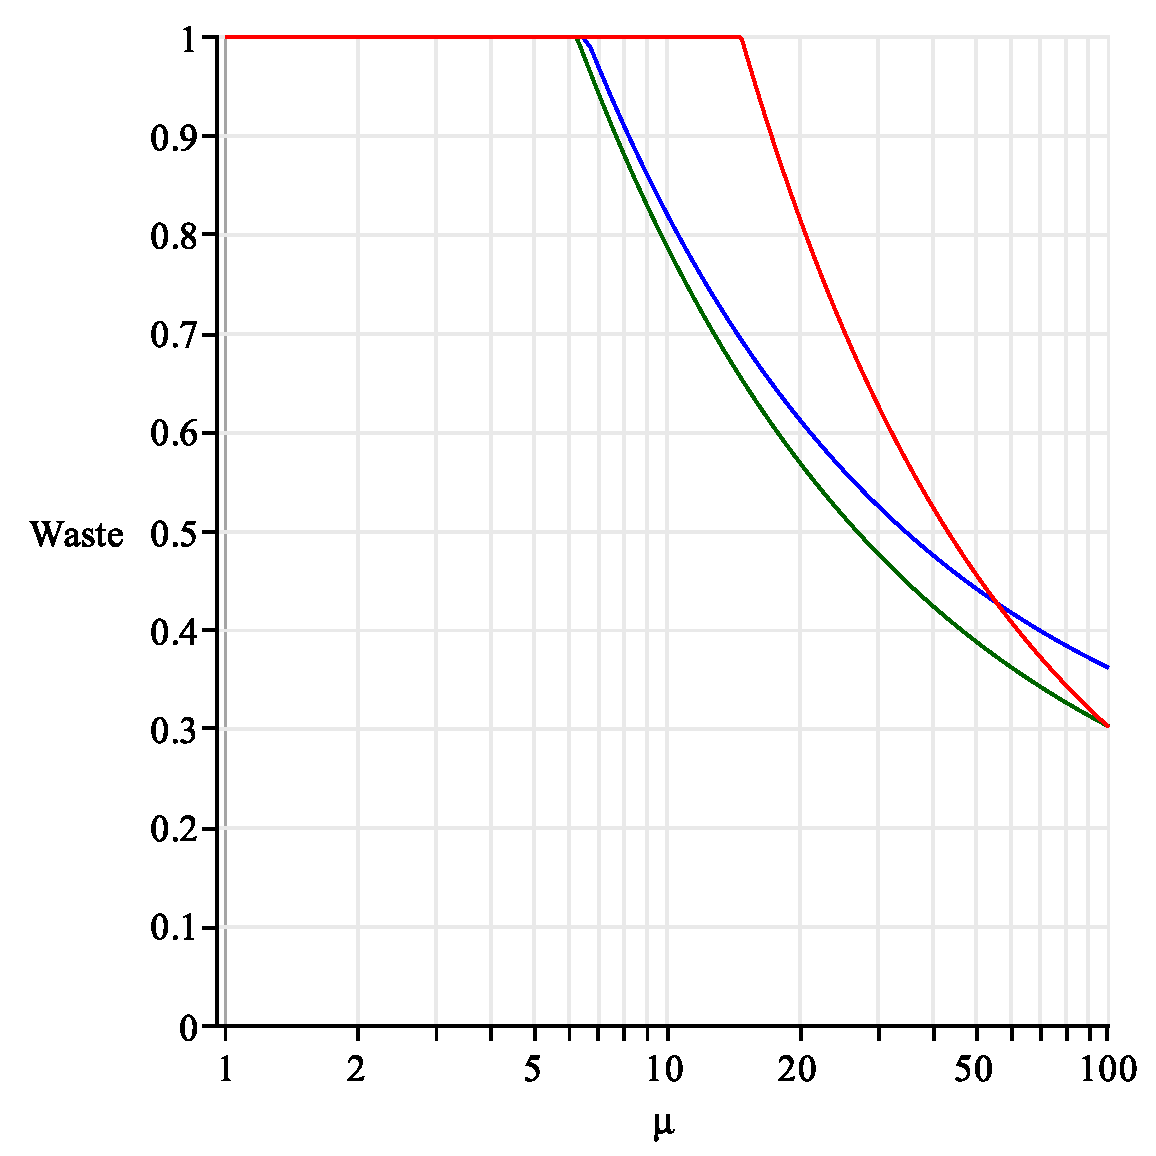
\includegraphics[width=0.3\textwidth,height=0.32\textheight,viewport=70 35 555 555,clip]{SlimWasteMat100.pdf} &
  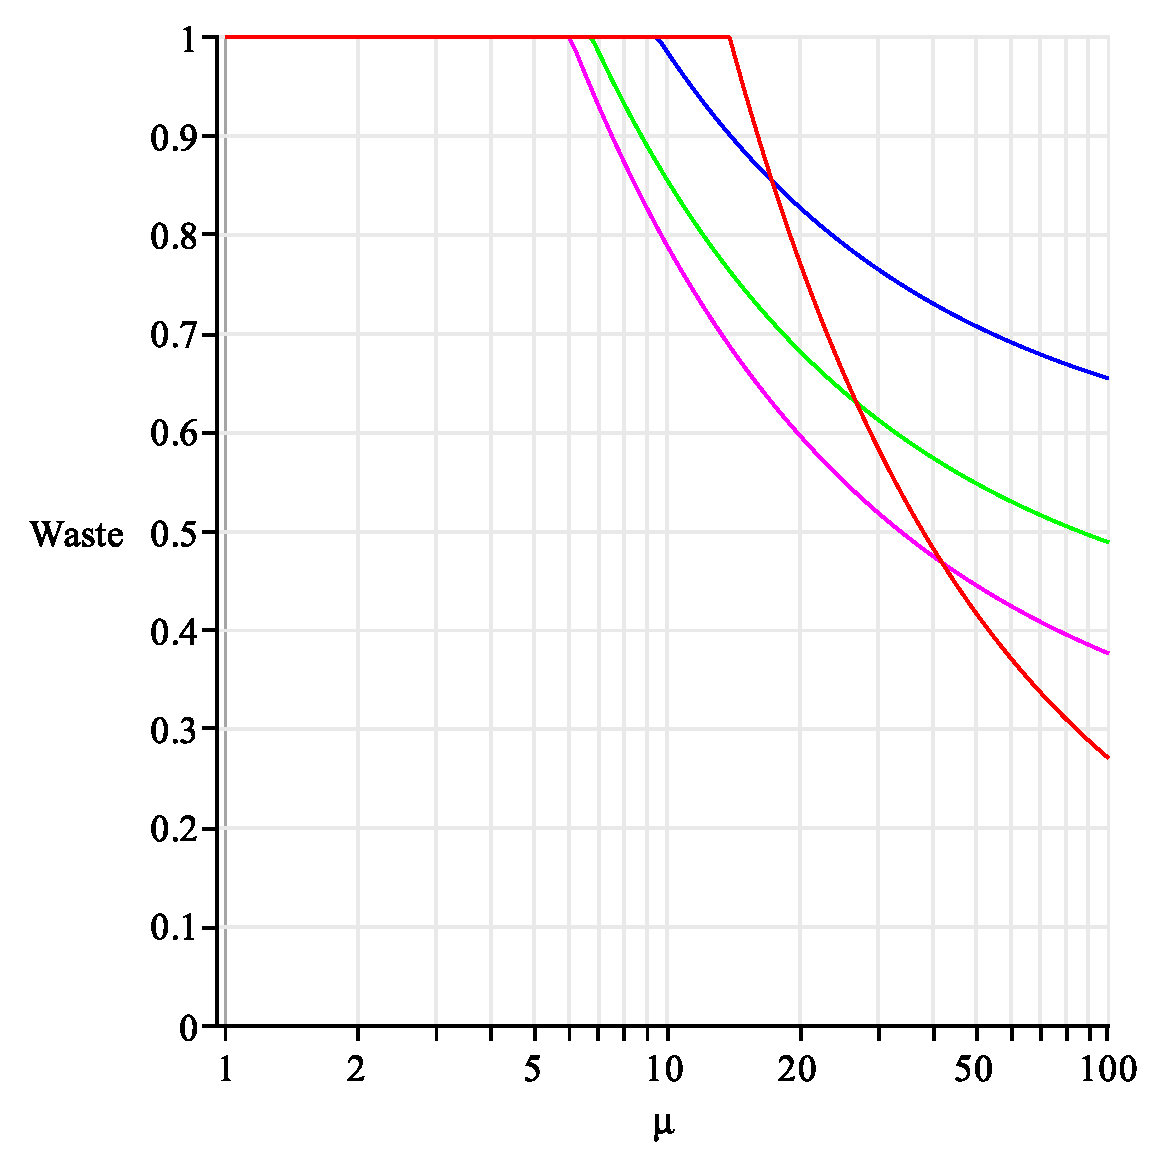
\includegraphics[width=0.3\textwidth,height=0.32\textheight,viewport=70 35 555 555,clip]{SlimWasteStenc3D100.pdf} \\
   \rotatebox{90}{\hspace{.5cm}Exascale-Fat} &
    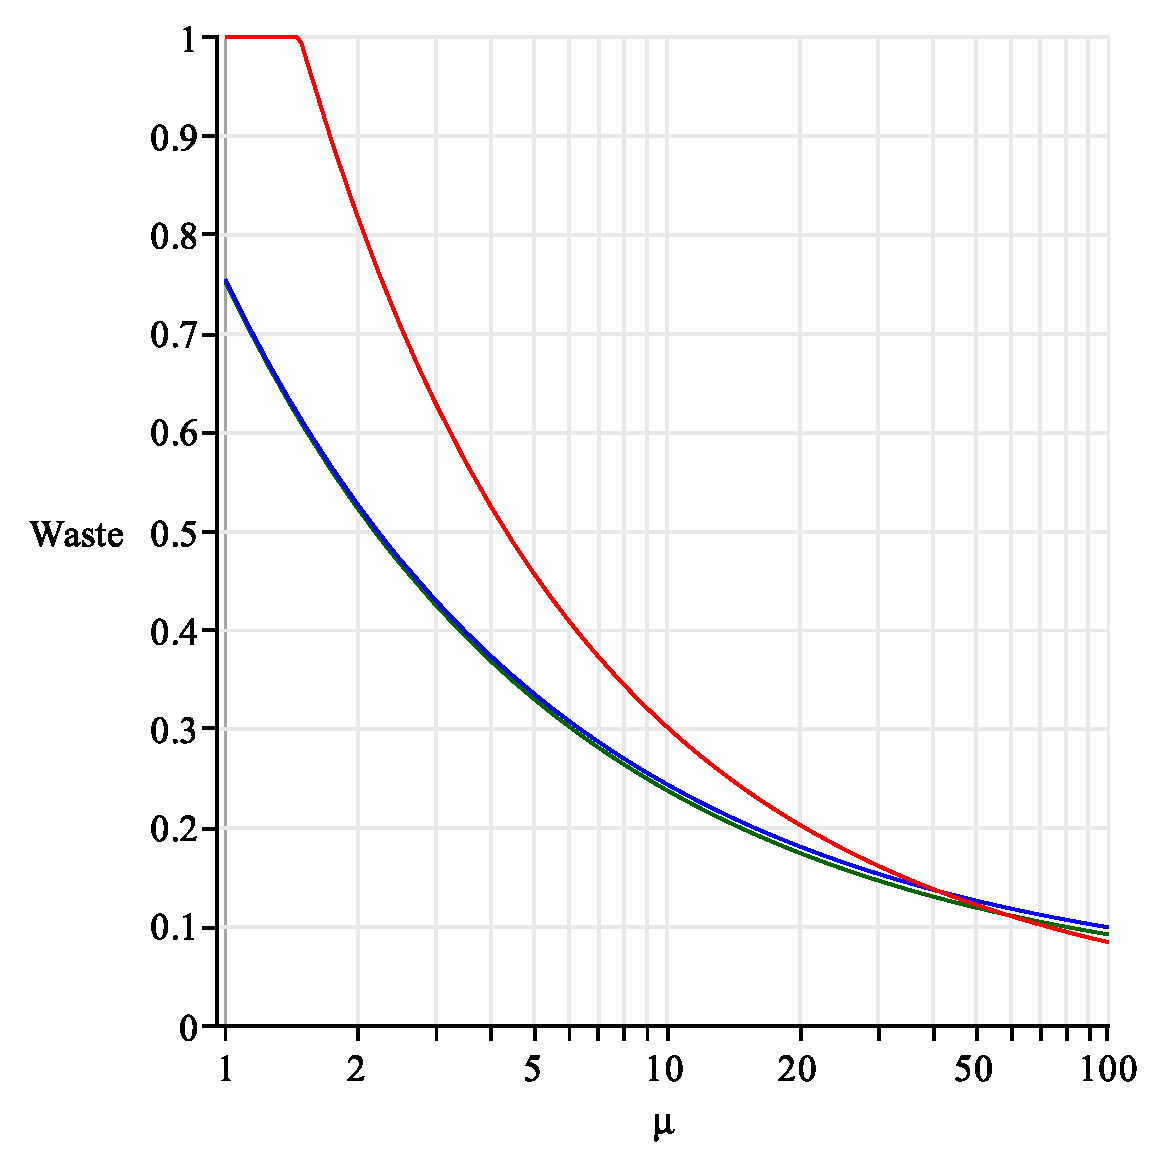
\includegraphics[width=0.3\textwidth,height=0.32\textheight,viewport=70 35 555 555,clip]{FatWasteStenc100.pdf} &
  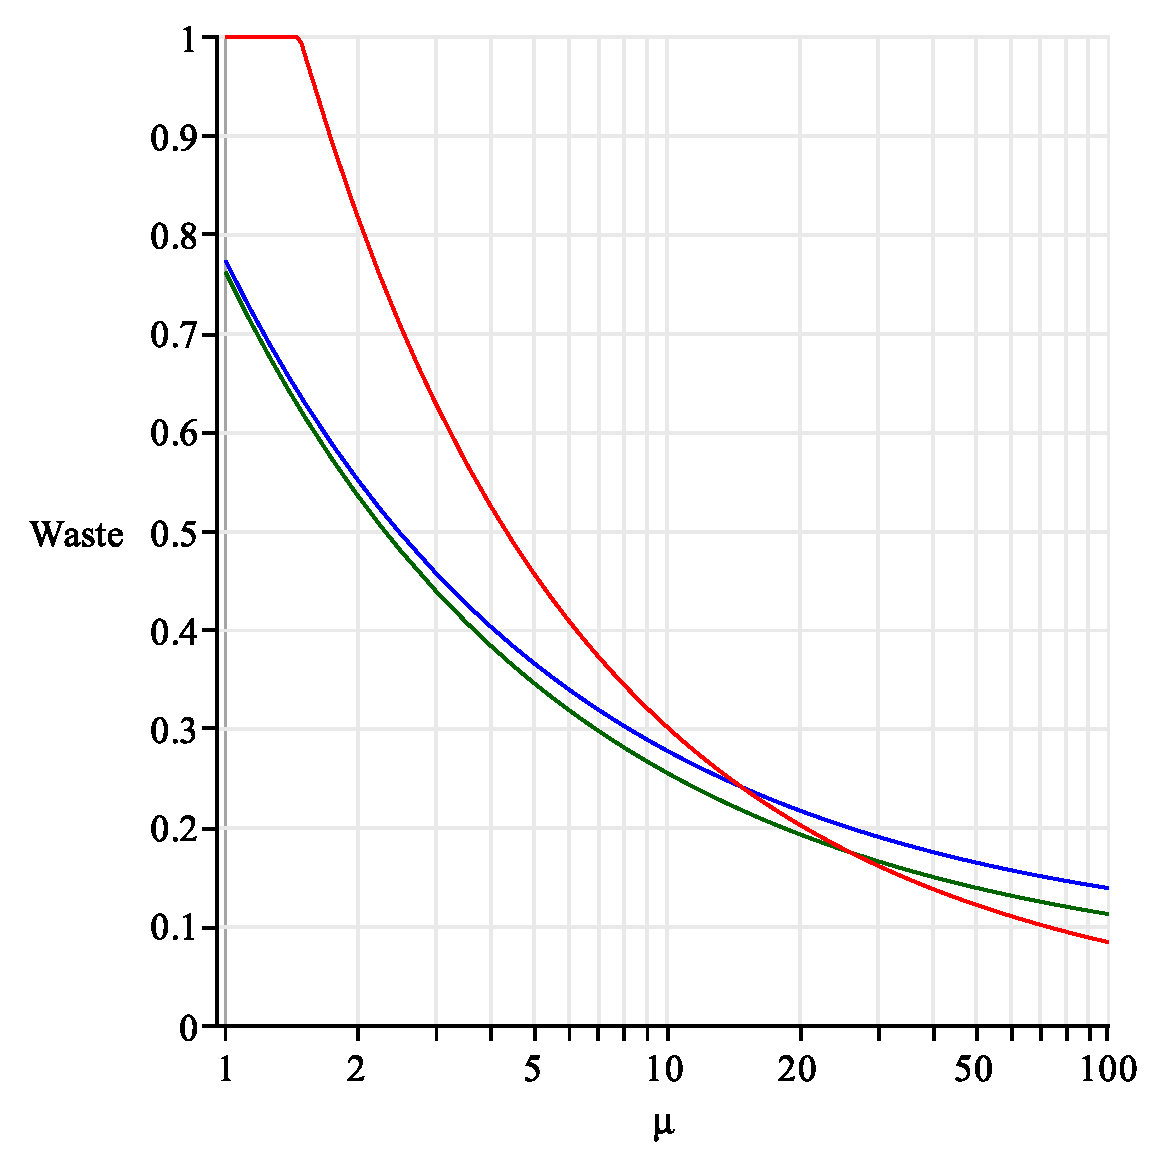
\includegraphics[width=0.3\textwidth,height=0.32\textheight,viewport=70 35 555 555,clip]{FatWasteMat100.pdf} &
  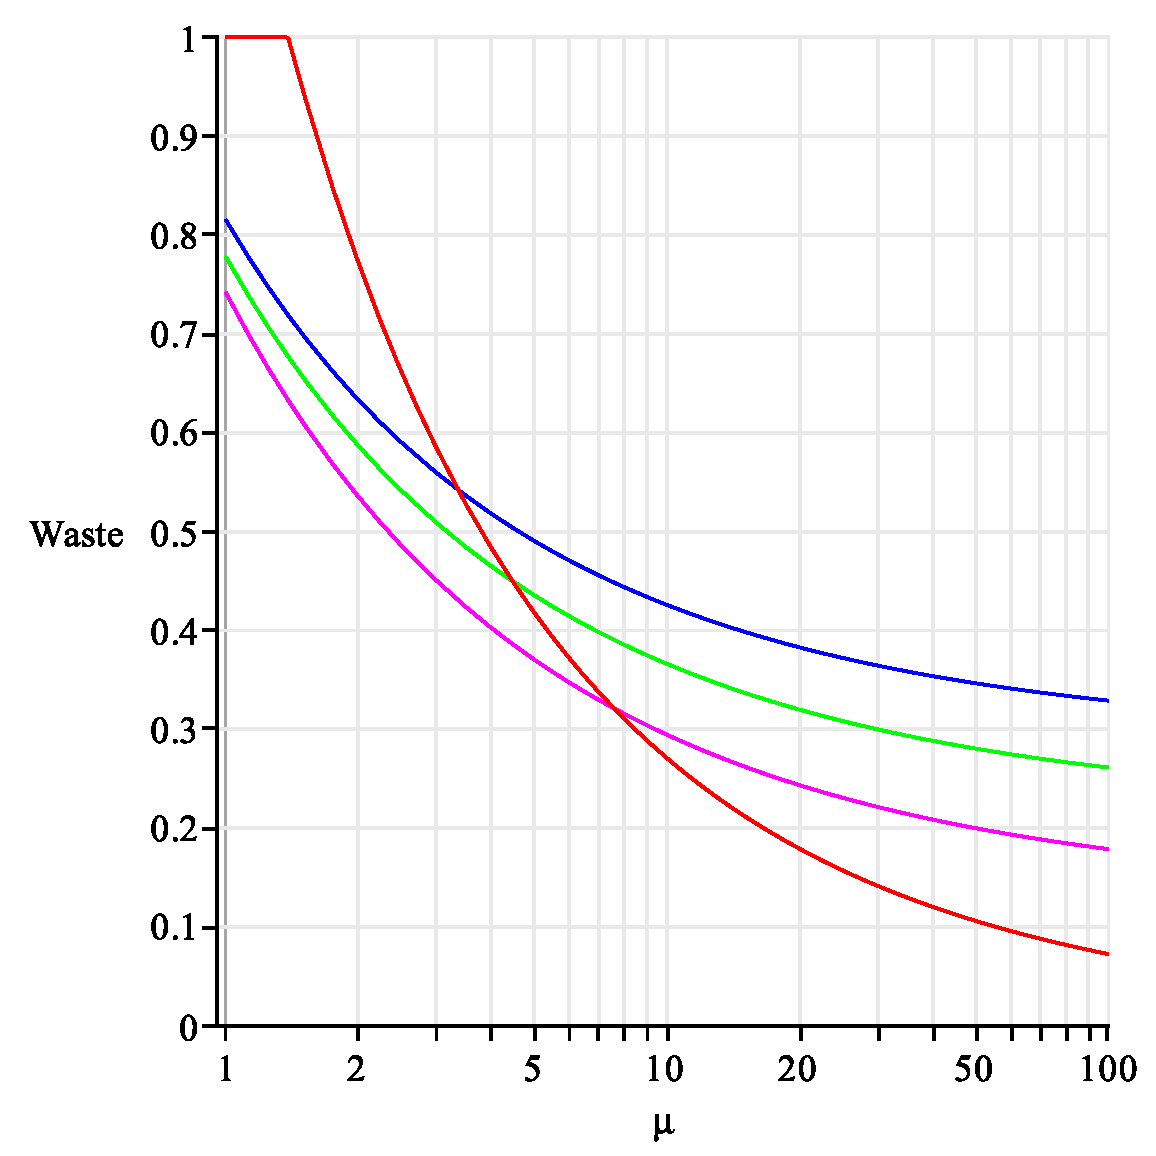
\includegraphics[width=0.3\textwidth,height=0.32\textheight,viewport=70 35 555 555,clip]{FatWasteStenc3D100.pdf} \\
 \end{tabular}
 ~\\
\centerline{Waste as a function of processor MTBF $\mu_{ind}$, $C=100$}
\end{frame}

\begin{frame}
  \frametitle{Conclusion on Hierarchical Checkpointing}

  \begin{itemize}
  \item Model for Hierarchical Checkpointing is \textcolor{red}{complex}
  \item Validation via simulation and comparison with few deployments
  \item \emph{All models are wrong, some are useful}
    \begin{itemize}
    \item Study highlights better resilience for \textcolor{blue}{fat} nodes for Exascale
    \item Narrow gap (\emph{application dependent}) of applicability for hierarchical approaches
    \end{itemize}
  \item Message Logging is doomed? See future work
  \end{itemize}
\end{frame}

\section{Application-Specific Fault Tolerance}

\begin{frame}
  \frametitle{ULFM: User-Level Failure Mitigation}

  \centering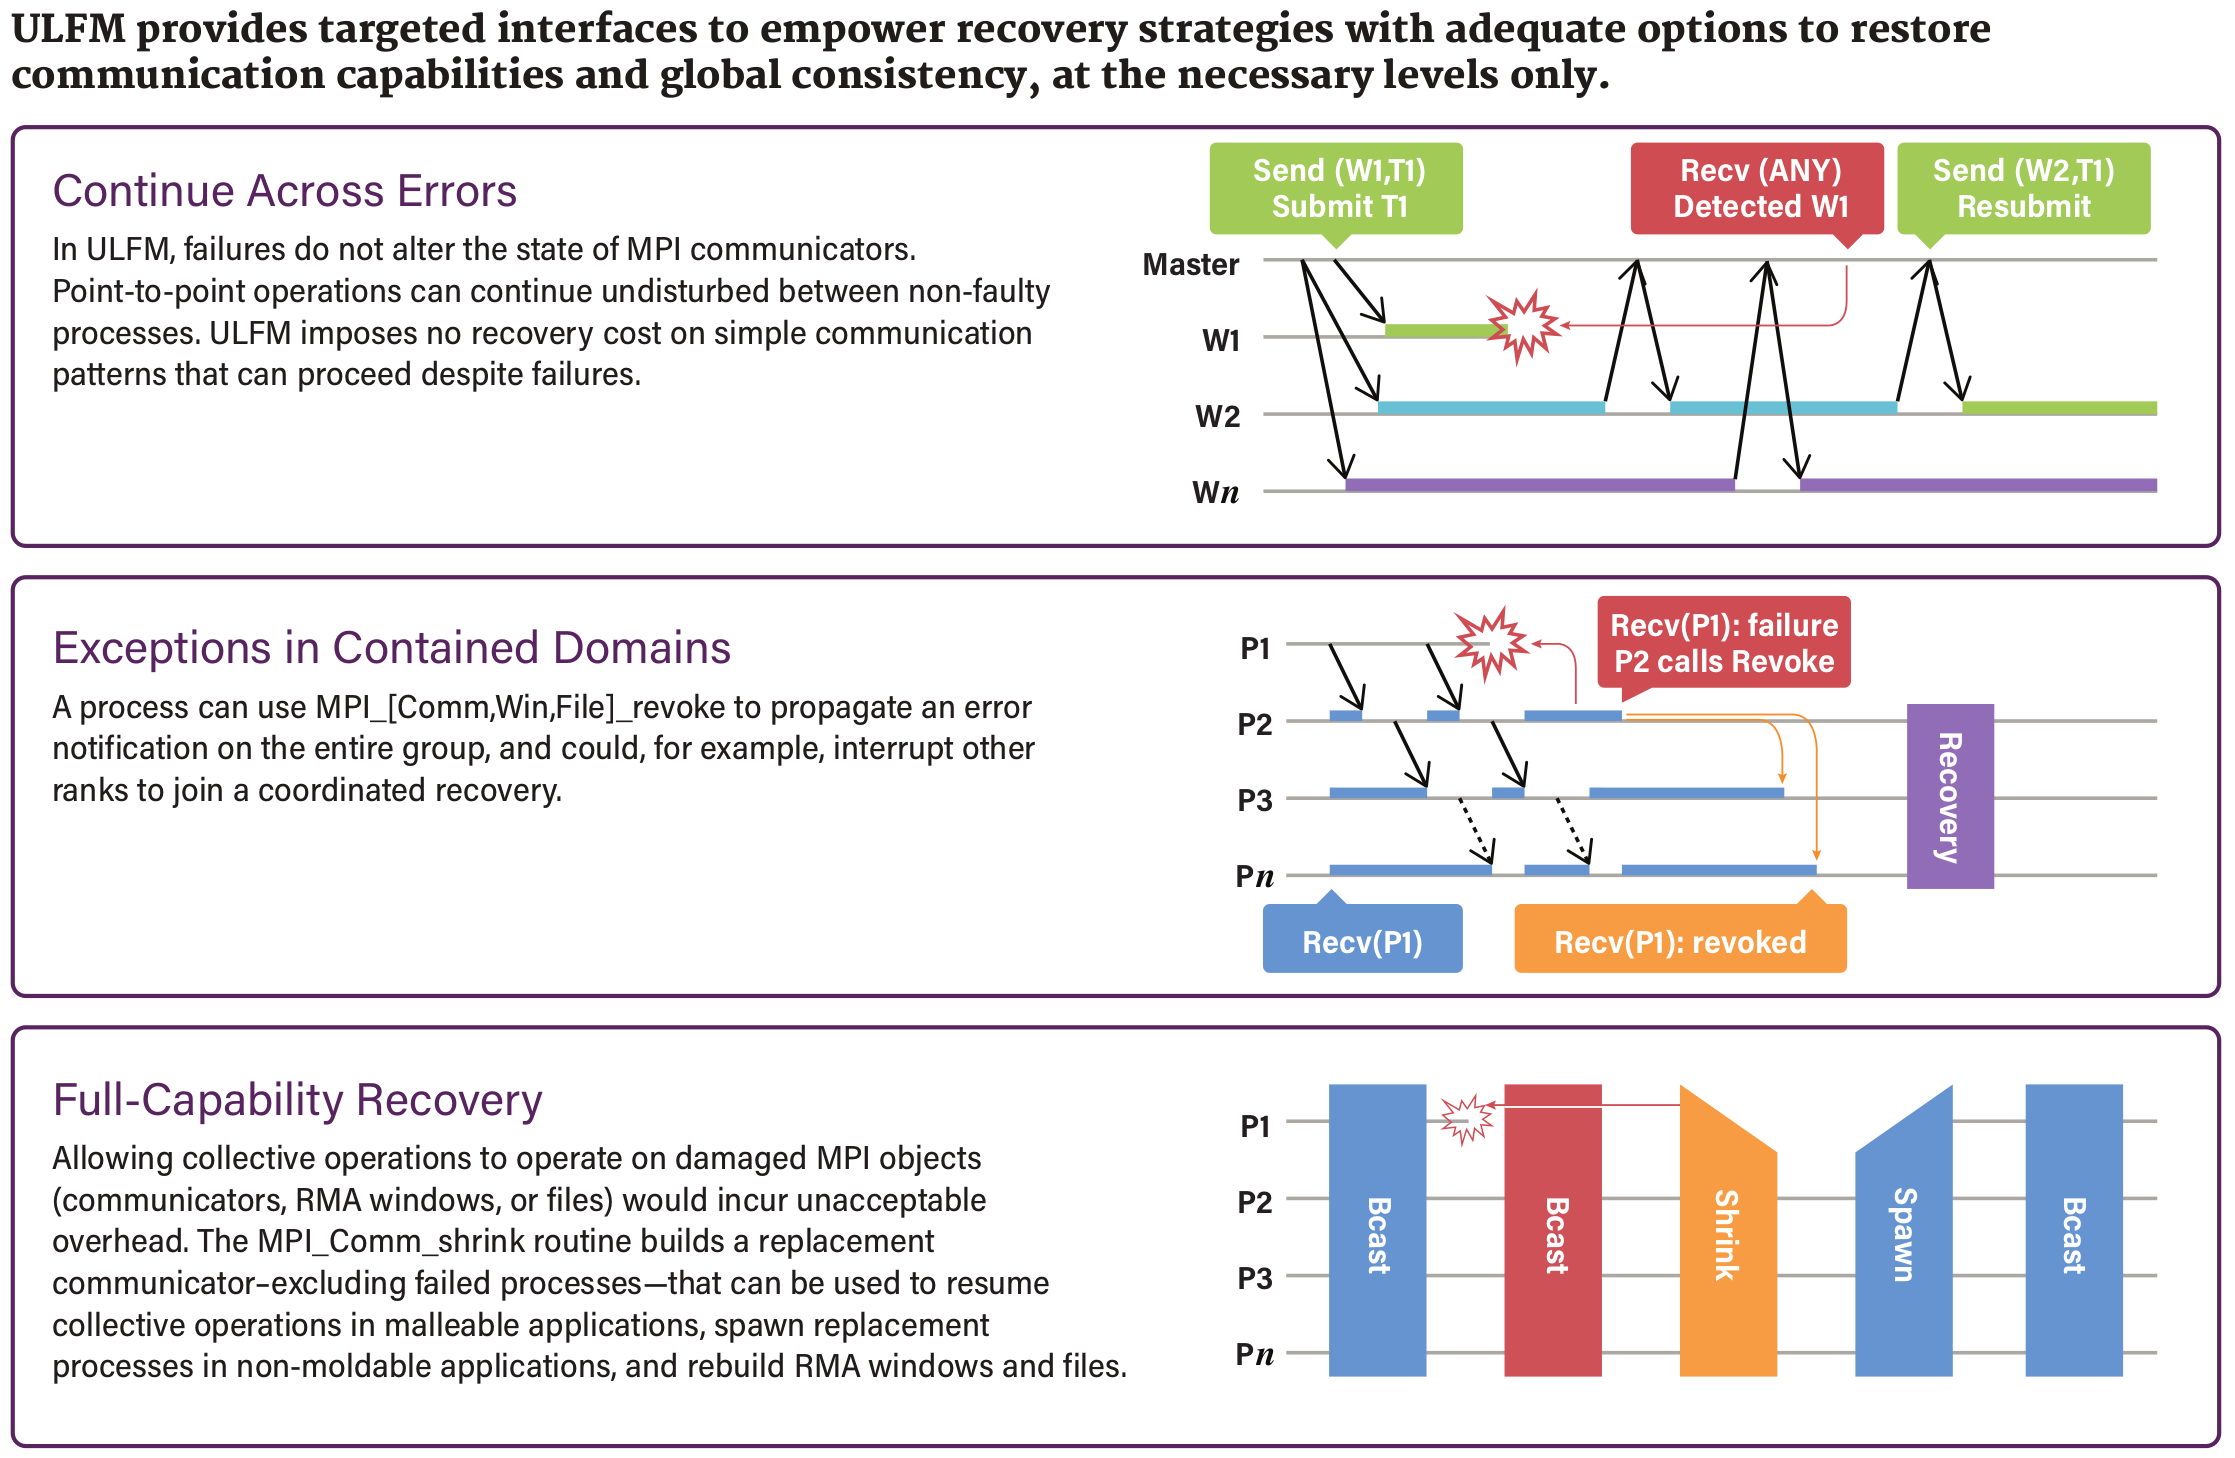
\includegraphics[height=.85\textheight]{ulfm.png}

\end{frame}

\subsection{Failure Detection and Notification}

\newcommand{\processes}{\ensuremath{{\mathcal P}}}
\newcommand{\status}[2]{\ensuremath{S_{#1}^{#2}}}
\newcommand{\emitter}{\ensuremath{\texttt{emitter}}\xspace}
\newcommand{\observer}{\ensuremath{\texttt{observer}}\xspace}
\newcommand{\alive}{\ensuremath{\texttt{alive}}\xspace}
\newcommand{\dead}{\ensuremath{\texttt{dead}}}
\newcommand{\heartbeat}{\ensuremath{\textsc{heartbeat}}\xspace}
\newcommand{\timeoutping}{\ensuremath{\textsc{HB-Timeout}}\xspace}
\newcommand{\timeoutsuspect}{\ensuremath{\textsc{Susp-Timeout}}\xspace}
\newcommand{\timeout}[1]{\ensuremath{\textsc{Timeout}_{#1}}\xspace}
\newcommand{\newobserver}{\ensuremath{\textsc{NewObserver}}\xspace}
\newcommand{\findpred}{\ensuremath{\textit{FindEmitter}}\xspace}
\newcommand{\neighbors}{\ensuremath{\textit{Neighbors}}\xspace}
\newcommand{\broadcastmsg}{\ensuremath{\textsc{BcastMsg}}\xspace}
\newcommand{\pinginterval}{\ensuremath{\eta}\xspace}
\newcommand{\msgtime}{\ensuremath{\tau}\xspace}
\newcommand{\suspectinterval}{\ensuremath{\delta}\xspace}
\newcommand{\emittors}[1]{\ensuremath{M(#1)}}
\newcommand{\ringemittor}[1]{\ensuremath{M_R(#1)}}
\newcommand{\additionalemittors}[1]{\ensuremath{M_A(#1)}}
\newcommand{\receivers}[1]{\ensuremath{O(#1)}}
\newcommand{\ringreceiver}[1]{\ensuremath{O_R(#1)}}
\newcommand{\additionalreceivers}[1]{\ensuremath{O_A(#1)}}
\newcommand{\transfer}[2]{\ensuremath{T_{#1,#2}}}
\newcommand{\deadmsg}[1]{\ensuremath{\texttt{DeadMsg(\ensuremath{#1})}}}
\newcommand{\broadcastneighbors}[1]{\ensuremath{\mathcal B}_{#1}}
\newcommand{\deads}[1]{\ensuremath{{\mathcal D}_{#1}}}
\newcommand{\muind}{\ensuremath{\mu_{\text{ind}}}}
\newcommand{\ringalgorithm}{\textsc{RingAlgorithm}}

\newcommand{\probaSymbol}{\mathbb P}
\newcommand{\proba}[1]{\probaSymbol\left(#1\right)}

\tikzset{
  pics/lightning/.style 2 args={code={
      \draw [arrows={-stealth[scale=2]}] (#1) -- 
      ($(#1)!.5!(#2) + (.05,-.05)$) -- 
      ($(#1)!.5!(#2) + (-.05,.05)$) --
      (#2);
}}}

\usetikzlibrary{shadows,patterns,shapes}
\definecolor{bluetheme}{RGB}{0,128,255}

\tikzstyle{fancytitle} = [fill=bluetheme!40, text=black, rounded corners,inner sep=4pt] 
\tikzstyle{mybox} = [draw=bluetheme!40, fill=bluetheme!20, very thick, rectangle, rounded corners, inner ysep=10pt, drop shadow]

\tikzstyle{fancytitleR} = [fill=bluetheme, text=black, rounded corners,inner sep=4pt] 

\tikzstyle{myboxTitle} = [draw=bluetheme, fill=bluetheme, very thick, rectangle, rounded corners, inner ysep=10pt, drop shadow]

\tikzstyle{myboxR} = [draw=bluetheme, fill=bluetheme!20, very thick, rectangle, rounded corners, inner ysep=10pt]


\begin{frame}
  \frametitle{ULFM: Failure Detection and Notification}
  \begin{itemize}
  \item Default Failure Detection: TCP time-out ($\sim 20mn$)
  \item Default Failure Notification: Admin network
  \item Work on \textcolor{red}{fail-stop} errors assumes  \textcolor{red}{\emph{instantaneous}} failure detection
  \item Goals:
    \begin{itemize}
    \item Continue execution after crash of \textbf{several} nodes
    \item Need \emph{rapid} and \emph{global} knowledge of group members
      \begin{enumerate}
      \item \textcolor{red}{Rapid}: failure detection
      \item \textcolor{red}{Global}: failure notification
      \end{enumerate}
    \item Resilience mechanism should \textcolor{blue}{have minimal impact}
    \end{itemize}
  \end{itemize}
\end{frame}

\begin{frame}
\frametitle{Timeout techniques: $p$ observes $q$}
\begin{columns}
\begin{column}{0.75\textwidth}
\begin{itemize}
\item Pull technique
\begin{itemize}
\item Observer $p$ sends a \emph{Are you alive} message to $q$
\item[\textcolor{red}{\frownie}] More messages
\item[\textcolor{red}{\frownie}] Long timeout
\end{itemize}
\end{itemize}
\end{column}
\begin{column}{0.3\textwidth}
\centering
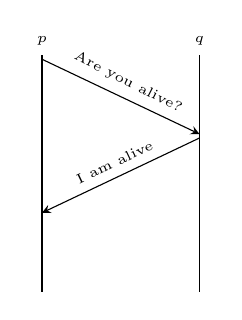
\begin{tikzpicture}
\draw (0, 3) -- (0, 0);
\node at (0,3) [font=\tiny,above]{$p$};
\draw (2, 3) -- (2, 0);
\node at (2,3) [font=\tiny,above]{$q$};
\draw [>=stealth,->] (0,2.95) -- (2,2) node [font=\tiny,midway,above,rotate=333] {Are you alive?};
\draw [>=stealth,->] (2,1.95) -- (0,1) node [font=\tiny,midway,above,rotate=25.40] {I am alive};
\end{tikzpicture}
\end{column}
\end{columns}

\begin{columns}
\begin{column}{0.75\textwidth}
\begin{itemize}
\item Push technique [1]
\begin{itemize}
\item Observed $q$ periodically sends heartbeats to $p$
\item[\textcolor{green}{\smiley}] Less messages
\item[\textcolor{green}{\smiley}] Faster detection (shorter timeout)
\end{itemize}
\end{itemize}
\end{column}
\begin{column}{0.3\textwidth}
\centering
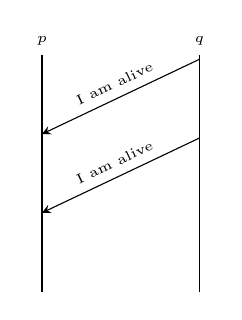
\begin{tikzpicture}
\draw (0, 3) -- (0, 0);
\node at (0,3) [font=\tiny,above]{$p$};
\draw (2, 3) -- (2, 0);
\node at (2,3) [font=\tiny,above]{$q$};
\draw [>=stealth,->] (2,2.95) -- (0,2) node [font=\tiny,midway,above,rotate=25.40] {I am alive};
\draw [>=stealth,->] (2,1.95) -- (0,1) node [font=\tiny,midway,above,rotate=25.40] {I am alive};
\end{tikzpicture}
\begin{tikzpicture}
\end{tikzpicture}
\end{column}
\end{columns}
\vfill
\scriptsize{[1]: W. Chen, S. Toueg, and M. K. Aguilera. On the quality of service of failure detectors. IEEE Trans. Computers, 2002}
\end{frame}

\begin{frame}
\frametitle{Algorithm for failure detection}

\begin{columns}
\begin{column}{0.5\textwidth}
\begin{itemize}
\item Processes arranged as a ring
\item Periodic heartbeats from a node to its successor
~\\
~\\
\item \textcolor{red}{Maintain ring of alive nodes}
\begin{itemize}
\item[$\rightarrow$] Reconnect ring after a failure
\item[$\rightarrow$] Inform all processes
\end{itemize}
\end{itemize}
\end{column}
\begin{column}{0.5\textwidth}
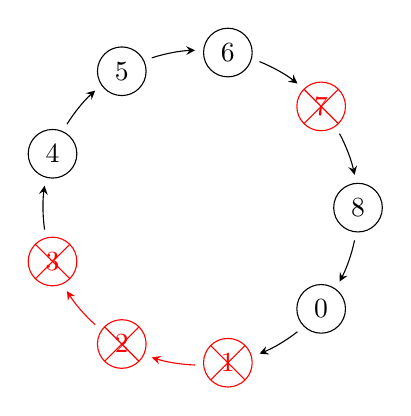
\begin{tikzpicture}[cross/.style={path picture={
  \draw[red]
(path picture bounding box.south east) -- (path picture bounding box.north west) (path picture bounding box.south west) -- (path picture bounding box.north east);
}}]
\def \n {9}
\def \radius {2cm}
\def \margin {12} 

\foreach \s in {1,...,\n}
{
  \pgfmathtruncatemacro\id{\n - \s}
  \ifthenelse{\s = 7 \OR \s = 6 \OR \s = 8 \OR \s = 2}
    {\node[draw, circle, red, cross] at ({360/\n * (\s - 1)}:\radius){$\id$};}
    {
        \ifthenelse{\s = 9}
                   {\node[draw, circle] at ({360/\n * (\s - 1)}:\radius){$0$};}
                   {\node[draw, circle] at ({360/\n * (\s - 1)}:\radius) {$\id$};};

    }
  \ifthenelse{\s = 6 \OR \s = 7}
  {\draw[->, >=stealth,red] ({360/\n * \s -\margin}:\radius)
    arc ({360/\n * \s - \margin}:{360/\n * (\s - 1)+\margin}:\radius);}
  {\draw[->, >=stealth] ({360/\n * \s - \margin}:\radius)
    arc ({360/\n * \s - \margin}:{360/\n * (\s - 1) + \margin}:\radius);}
}
\end{tikzpicture}
\end{column}
\end{columns}
\end{frame}




%\section{Failure propagation}



\begin{frame}
\frametitle{Reconnecting the ring}
\centering
\begin{overlayarea}{\textwidth}{\textwidth}
  {
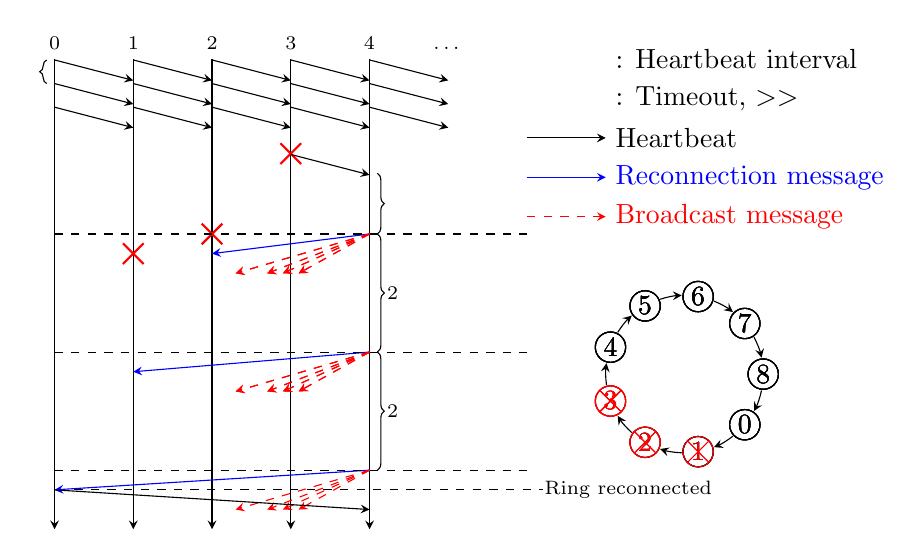
\begin{tikzpicture}[cross/.style={path picture={
  \draw[red]
(path picture bounding box.south east) -- (path picture bounding box.north west) (path picture bounding box.south west) -- (path picture bounding box.north east);
}}]
%%%%% position of the first process and distance between processes
%\begin{minipage}[t]{0.5\textwidth}
\def\z{0}
\def\s{1}
%%%%% lenght of the execution
\def\total{8}
%%%%% delta duration
\def\Tau{0.25}
\def\Eta{0.3}
\def\l{\total-4*\Eta}
\def\Delta{0.75}
%%%failure begin coordinate
\def\fb{0.01}
%%%failure end coordinate
\def\fe{0.50}
%%%% dashed lines for delta
\def\f{0.3}
%%%% number of faults
\def\nbf{3}
\def\propag{0.50}
\pgfmathsetmacro{\nbfmo}{\nbf - 1};
%%%%% beginning of reconnection tentative
\pgfmathsetmacro{\detect}{2 * \Delta}
\def\BeginRec{\l - \fb -\fb - \Tau - \Delta}
\def\Failure3{\BeginRec - \Tau - \Delta - \detect}
\def\EndRec{ \BeginRec - \nbfmo * \detect - \Tau - 2 * \Tau}
%\def\EndRec{\BeginBcast - \nbfmo * \propag - \propag}

%%failure free
  \draw [>=stealth,->] (\z - \s,\total) -- (\z - \s, \EndRec);
  \node at (\z - \s,\total) [font=\scriptsize,above]{$0$};

  \onslide<1-5>{\draw [>=stealth,->] (\z,\total) -- (\z, \EndRec);}
  \node at (\z,\total) [font=\scriptsize,above]{$1$};
\node [right] at (\z + 6, \total) {$\pinginterval$: Heartbeat interval};

\onslide<1-4>{\draw [>=stealth,->] (\z + \s,\total) -- (\z +\s, \EndRec);}
  \node at (\z + \s,\total) [font=\scriptsize,above]{$2$};

\draw [decoration={brace,mirror}, decorate] (\z - \s - 0.10,\total - \fb) -- (\z - \s - 0.10,\total - \fb - \Eta) node [black,midway, 
 left,font=\scriptsize,align=left]{$\pinginterval$};

\onslide<1>{\draw [>=stealth,->] (\z + 2*\s,\total) -- (\z + 2*\s, \EndRec);};
  \node at (\z + 2 * \s, \total) [font=\scriptsize,above]{$3$};

  \draw [>=stealth,->] (\z + 3*\s,\total) -- (\z + 3*\s, \EndRec);
  \node at (\z + 3*\s,\total) [font=\scriptsize,above]{$4$};
  \node at (\z + 4*\s,\total) [font=\scriptsize,above]{\ldots};
\draw [>=stealth,->] (\z + 5, \total - 1) -- (\z + 6, \total - 1) node [right]{Heartbeat};

\foreach \y in {0, 1, 2}
{
\foreach \x in {-1,0,1,2,3}
{  
  \draw  [>=stealth,->] (\z + \x * \s, \total - \fb - \y * \Eta) -- (\z+\x*\s+\s, \total - \fb - \fb - \Tau - \y * \Eta) node [font=\tiny,midway,rotate=331,below]{};
}
}

\onslide<2->{
%% failure of 3

  %  \draw (\z + 2*\s,\total) -- (\z + 2*\s, \l);
  \draw (\z + 2*\s,\total) -- (\z + 2*\s, \total-4*\Eta);
  \draw (\z + 2 * \s,\l) -- (\z + 2 * \s, \l) node [cross out, draw, red,
  thick]{};
  \onslide<3->{\draw [decoration={brace}, decorate] (\z + 3*\s + 0.10,\l - \Tau) -- (\z + 3*\s + 0.10,\BeginRec) node [black,midway, 
  right,font=\scriptsize,align=left]{$\suspectinterval$};}

  \onslide<5->{\draw (\z + \s,\total) -- (\z +\s, \BeginRec) node [cross out, draw, red,
  thick]{};}

\onslide<6->{
\draw (\z,\total) -- (\z,  \BeginRec - \Tau) node [cross out, draw, red,
  thick]{};;}

\draw  [>=stealth,->] (\z + 2*\s, \l - \fb) -- (\z+3*\s, \l - \fb - \fb - \Tau );

\foreach \x in {2,1,0}
{
  \pgfmathtruncatemacro{\y}{2 - \x};
  \pgfmathtruncatemacro{\i}{\x - 1};
  \pgfmathtruncatemacro{\anim}{\y + 3 + 1};

  \ifthenelse{\NOT \x = 0}
             {\onslide<\anim->{\draw [>=stealth,->,blue] (\z + 3 * \s, \BeginRec - \y * \detect) -- (\z + \i * \s, \BeginRec - \Tau - \y * \detect) node [font=\tiny,midway,rotate=15,below]{};
                 \onslide<7>{
                   \foreach \q in {1, 2, 3}
                      {
                        \draw [dashed,red,>=stealth,->] (\z + 3*\s,\BeginRec - \y * \detect) -- (\z + 1.5 *\s + 0.2*\q,\BeginRec - \y * \detect - \propag);
                      }
                      \draw [dashed,red,>=stealth,->] (\z + 3*\s,\BeginRec - \y * \detect) -- (\z + 1.3 *\s,\BeginRec - \y * \detect - \propag);
             }}}
             {\onslide<\anim->{\draw [>=stealth,->,blue] (\z + 3 * \s, \BeginRec - \y * \detect) -- (\z + \i * \s, \BeginRec - \Tau - \y * \detect) node [font=\tiny,midway,rotate=10,above]{};}}
             \pgfmathtruncatemacro{\anime}{\y + 4};
             \onslide<\anime->{\draw[dashed](\z -\s, \BeginRec - \y * \detect) -- (\z + 5*\s,  \BeginRec - \y * \detect);
               \ifthenelse{\y > 0}
                          {\draw [decoration={brace,mirror}, decorate] (\z + 3*\s + 0.10, \BeginRec - \y * \detect) -- (\z + 3*\s + 0.10, \BeginRec - \y * \detect + \detect) node [black,midway, 
                              right,font=\scriptsize,align=left]{2$\suspectinterval$};}{}
             }
             \onslide<\anim->{
               \onslide<7>{
                 \foreach \q in {1, 2, 3}
                    {
                      \draw [dashed,red,>=stealth,->] (\z + 3*\s,\BeginRec - \y * \detect) -- (\z + 1.5 *\s + 0.2*\q,\BeginRec - \y * \detect - \propag);
                    }
                    \draw [dashed,red,>=stealth,->] (\z + 3*\s,\BeginRec - \y * \detect) -- (\z + 1.3 *\s,\BeginRec - \y * \detect - \propag);
             }}
             \ifthenelse{\NOT \x = 0}{}
                        {\onslide<\anim->{
                            \draw [dashed] (-0.75, \BeginRec - \nbfmo * \detect - \Tau) -- (\z + 5 * \s + 0.20, \BeginRec - \nbfmo * \detect - \Tau);
                            \draw (\z + 5*\s + 0.10, \BeginRec - \nbfmo * \detect - \Tau) node [font=\scriptsize,right]{Ring reconnected}; 
%%%heartbeat of the healthy process
                            \draw  [>=stealth,->] (\z-\s, \BeginRec - \nbfmo * \detect - \Tau) -- (\z + 3*\s,  \BeginRec - \nbfmo * \detect - \Tau - \Tau) node [font=\tiny,midway,rotate=350,below]{};}
                        }
}

\onslide<3->{\node [right] at (\z + 6, \total-0.5) {$\suspectinterval$: Timeout, $\suspectinterval >> \msgtime$};}
%\node [left,font=\scriptsize] at (\z + 6, \total-2) {$\msgtime$: Message transmission upper bound};}
\onslide<4->{\draw [>=stealth,->,blue ](\z + 5, \total-1.5) -- (\z + 6, \total-1.5) node [right]{Reconnection message};}
\onslide<7->{\draw [>=stealth,->,dashed,red ](\z + 5, \total-2) -- (\z + 6, \total-2) node [right]{Broadcast message};}

%%% T(3)
%% \draw [dashed] (-0.75, \l - \fb - \fb) -- (3, \l - \fb - \fb);
%% \draw [dashed] (-0.75, \EndRec) -- (3, \EndRec);
%% \draw [>=stealth,<->] (-0.75, \l - \fb - \fb) -- (-0.75, \EndRec) node [font=\scriptsize,left,midway]{$T(\nbf,C)$};

%% \draw (3.25, \EndRec - 0.10) rectangle (6.25,\EndRec - 0.65 - 0.10 - 0.20);
%% \draw node at (3.25, \EndRec - 0.10 - 0.15) [font=\scriptsize,right]{HB=\heartbeat};
%% \draw node at (3.25, \EndRec - 0.10 - 0.40) [font=\scriptsize,right,blue]{NO=\newobserver};
%% \draw node at (3.25, \EndRec - 0.10 - 0.65) [font=\scriptsize,right,red]{Bcast=Broadcast Operation};
}

\def \n {9}
\def \radius {1}
\def \margin {12}
%\node[circle, red, cross,right of=fin] at ({360/\n * 2 - 110}:\radius){7};
%\node[circle, red, cross,right of=fin] at ($(fin.south west)+(3,0)$){6};
\draw node at (\z + 5*\s,  \BeginRec - \detect)(fin){};
%\node(A)[draw,circle,right of=fin,xshift=1cm,yshift=1cm]{0};

\foreach \s in {1,...,\n}
{
  \pgfmathtruncatemacro\id{\n - \s}
  \onslide<1>{
    \node[draw, circle,right of=fin,xshift=6cm,yshift=4cm,inner sep=1pt] at ({360/\n * (\s - 1)}:\radius) {$\id$};
  }
  \onslide<2-4>{
    \ifthenelse{\id = 3}
       {\node[draw,circle, red, cross,right of=fin,xshift=6cm,yshift=4cm,circle,inner sep=1pt] at ({360/\n * (\s - 1)}:\radius){$\id$};}
       {
         \node[draw, circle,right of=fin,xshift=6cm,yshift=4cm,inner sep=1pt] at ({360/\n * (\s - 1)}:\radius) {$\id$};
       }
  }
  \onslide<5>{
    \ifthenelse{\id = 3 \OR \id=2}
             {\node[draw,circle, red, cross,right of=fin,xshift=6cm,yshift=4cm,circle,inner sep=1pt] at ({360/\n * (\s - 1)}:\radius){$\id$};}
             {
               \node[draw, circle,right of=fin,xshift=6cm,yshift=4cm,inner sep=1pt] at ({360/\n * (\s - 1)}:\radius) {$\id$};
             }
  }
  \onslide<6->{
    \ifthenelse{\id = 3 \OR \id=2 \OR \id=1}
               {\node[draw,circle,red,cross,right of=fin,xshift=6cm,yshift=4cm,circle,inner sep=1pt] at ({360/\n * (\s - 1)}:\radius){$\id$};}
               {
                 \node[draw, circle,right of=fin,xshift=6cm,yshift=4cm,inner sep=1pt] at ({360/\n * (\s - 1)}:\radius) {$\id$};
               }
  }
%% \ifthenelse{\s = 6 \OR \s = 7}
  %% {\draw[->, >=stealth,red] ({360/\n * \s -\margin}:\radius)
  %%   arc ({360/\n * \s - \margin}:{360/\n * (\s - 1)+\margin}:\radius);}%|- (\z+5,\total-2)
  \draw[->, >=stealth,xshift=7cm,yshift=4cm] ({360/\n * \s - \margin}:\radius)
    arc ({360/\n * \s - \margin}:{360/\n * (\s - 1) + \margin}:\radius);
}

\end{tikzpicture}
}
\end{overlayarea}
\end{frame}

\begin{frame}
  \frametitle{Failure Notification}

  \begin{columns}
    \begin{column}{0.6\textwidth}
      \begin{itemize}
      \item Hypercube Broadcast Algorithm
        \begin{itemize}
        \item Recursive doubling broadcast algorithm by each node
        \item Completes if $f \leq \lfloor log(n)\rfloor - 1$ ($f$: number of failures, $n$: number of alive processes)
        \item Completes within $2 \tau log(n)$
        \end{itemize}
        \vfill
      \item Application to failure detector
        \begin{itemize}
        \item If $n \neq 2^l$
          \begin{itemize}
          \item $k = \lfloor log(n) \rfloor$ 
          \item $2^k \leq  n  \leq 2^{k+1}$
          \item Initiate two successive broadcast operations
          \end{itemize}
        \item Source $s$ of broadcast sends its current list $D$ of dead processes
        \item {\scriptsize No update of $D$ during broadcast initiated by $s$ -- (do NOT change broadcast topology on the fly)}
        \end{itemize}
      \end{itemize}
    \end{column}

    \begin{column}{0.4\textwidth}
      \centering
      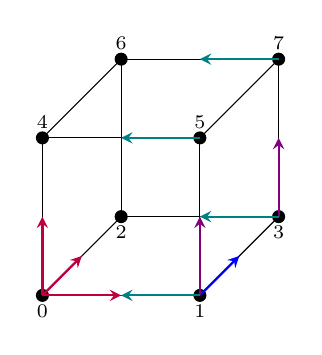
\begin{tikzpicture}
        \def\size{2}
        \def\decalage{1}
        \def\arrowLength{1}
        \foreach \x in {0, 1}
                 {
                   \draw (\x*\decalage,\size+\x*\decalage) -- (\size+\x*\decalage,\size+\x*\decalage);
                   \node [circle,fill=black,scale=0.5] at (\x*\decalage,\size+\x*\decalage){};
                   \pgfmathtruncatemacro{\id}{\x*\decalage*2+4};
                   \node [above,font=\scriptsize] at  (\x*\decalage,\size+\x*\decalage){\id};%{\pgfmathparse{\x*\decalage*2+4}\pgfmathresult};
                   \draw (\x*\decalage,\x*\decalage) -- (\x*\decalage,\size+\x*\decalage);
                   \node [circle,fill=black,scale=0.5] at (\x*\decalage,\x*\decalage){};
                   \pgfmathtruncatemacro{\id}{\x*\decalage*2};
                   \node [below,font=\scriptsize] at (\x*\decalage,\x*\decalage){\id};
                   \draw (\size+\x*\decalage,\size+\x*\decalage) -- (\size+\x*\decalage,\x*\decalage);
                   \node [circle,fill=black,scale=0.5] at (\size+\x*\decalage,\size+\x*\decalage){};
                   \pgfmathtruncatemacro{\id}{\x*\decalage*2+5};
                   \node [above,font=\scriptsize] at (\size+\x*\decalage,\size+\x*\decalage){\id};
                   \draw (\x*\decalage,\x*\decalage) -- (\size+\x*\decalage,\x*\decalage);
                   \node [circle,fill=black,scale=0.5] at (\size+\x*\decalage,\x*\decalage){};
                   \pgfmathtruncatemacro{\id}{\x*\decalage*2+1};
                   \node [below,font=\scriptsize] at (\size+\x*\decalage,\x*\decalage){\id};
                 }
        \draw(0, \size) -- (\decalage, \size+\decalage);
        \draw(\size, \size) -- (\decalage+\size, \size+\decalage);
        \draw(0, 0) -- (\decalage, \decalage);
        \draw(\size, 0) -- (\size+\decalage, \decalage);
        \draw [>=stealth,->,purple,thick] (0,0) -- (\arrowLength,0);
        \draw [>=stealth,->,purple,thick] (0,0) -- (0,\arrowLength);
        \draw [>=stealth,->,purple,thick] (0,0) -- (\arrowLength/2,\arrowLength/2);
        \draw [>=stealth,->,blue,thick] (\size,0) -- (\arrowLength/2+\size,\arrowLength/2);
        \draw [>=stealth,->,violet,thick] (\size,0) -- (\size,\arrowLength);
        \draw [>=stealth,->,violet,thick] (\size+\decalage,\decalage) -- (\size+\decalage,\decalage+\arrowLength);
        \draw [>=stealth,->,teal,thick] (\size,0) -- (\arrowLength,0);
        \draw [>=stealth,->,teal,thick] (\size+\decalage,\decalage) -- (\arrowLength+\decalage,\decalage);
        \draw [>=stealth,->,teal,thick] (\size,\size) -- (\size-\arrowLength,\size);
        \draw [>=stealth,->,teal,thick] (\size+\decalage,\size+\decalage) -- (\size-\arrowLength+\decalage,\size+\decalage);
      \end{tikzpicture}

      \scriptsize
      \begin{tabular}{|c|c|c|c|}
        \hline
        Node & Node1 & Node2 & Node4\\\hline
        1 & \onslide<1->0 & \onslide<1->{0-2-3} &  \onslide<1->{0-4-5}\\
        2 & \onslide<1->{0-1-3} & \onslide<1->0 & \onslide<1->{0-4-6}\\
        3 & \onslide<1->{0-1} & \onslide<1->{0-2} & \onslide<1->{0-4-5-7}\\
        4 & \onslide<1->{0-1-5} & \onslide<1->{0-2-6} & \onslide<1-> 0\\
        5 & \onslide<1->{0-1} & \onslide<1->{0-2-6-7} & \onslide<1->{0-4}\\
        6 & \onslide<1->{0-1-3-7} & \onslide<1->{0-2} & \onslide<1->{0-4}\\
        7 & \onslide<1->{0-1-3} & \onslide<1->{0-2-6} & \onslide<1->{0-4-5}\\\hline
        \end{tabular}
    \end{column}
  \end{columns}

\end{frame}

\begin{frame}
\frametitle{Worst-case analysis}
\begin{center}
\begin{tikzpicture}
\node [mybox] (box) { %
  \begin{minipage}{1.0\textwidth}
\textbf{Stable configuration:}  \textcolor{red}{all dead nodes are known to all processes}
  \end{minipage}
};
\node [fancytitle, right=10pt] at (box.north west) {\text{\emph{Definition}}};
\end{tikzpicture}
  
\begin{tikzpicture}
\draw [>=stealth,|->](0,5) -- (10,5) node [font=\tiny,below left]{Time}; 
\draw (3,5.10) -- (3,4.90);
\node at (1.50,4.90)[below,font=\scriptsize]{Stable};
\draw (8,5.10) -- (8,4.90);
\node at (9,4.90)[below,font=\scriptsize]{Stable};
\node at (5.5,4.90)[below,font=\scriptsize]{at most $T(f)$ if $f$ faults};
\pic [red] {lightning={3.20,5.5}{3,5}};
%\draw [>=stealth, ->] (3.5, 5.5) -- (3, 5) ;
\pic [red] {lightning={3.70,5.5}{3.5,5}};
\pic [red] {lightning={4.20,5.5}{4,5}};
\node at (3.5,5.5) [above,font=\tiny]{Failures};
\pic [red] {lightning={5.20,5.5}{5,5}};
\pic [red] {lightning={5.70,5.5}{5.5,5}};
\pic [red] {lightning={7.2,5.5}{7,5}};

%\draw [>=stealth,->](0,5) -- (5,10) node [font=\tiny,below left]{Time}; 
\end{tikzpicture}
\end{center}

\begin{theorem}
With $n \leq N$ alive nodes, and for any $f \leq \lfloor \log n \rfloor -1$,
we have
\begin{equation*}
T(f) \leq  f(f+1)  \suspectinterval + f \msgtime + \frac{f(f+1)}{2}(8 \msgtime \log n)
\end{equation*}
\end{theorem}
\begin{itemize}
\item 2 sequential broadcasts: $4 \tau log n$
\item One-port model: broadcast messages and heartbeats interleaved
\end{itemize}

\end{frame}

\begin{frame}
\frametitle{Worst-case scenario}

$$\begin{array}{cccc}
T(f) \leq  & \underbrace{f(f+1)  \suspectinterval  +   f \msgtime}  & + &  \underbrace{\frac{f(f+1)}{2}(8 \msgtime \log n)}\\
& \textcolor{red}{reconstruction} & & \textcolor{blue}{broadcast}
\end{array}$$

\begin{itemize}
\item $T(f) \leq  \text{ring reconstruction} + \text{broadcasts}$ (for the proof)
\item \textcolor{blue}{Process $p$ discovers the death of $q$ at most \textbf{once}\\
$\Rightarrow$ $i-th$ dead process discovered dead by at most $f-i+1$ processes\\
$\Rightarrow$ at most $\frac{f(f+1)}{2}$ broadcasts}
\item \textcolor{red}{$R(f)$ ring reconstruction time\\
For $ 1 \leq f \leq \lfloor \log n \rfloor -1$,
$$R(f) \leq  R(f-1) + 2f  \suspectinterval + \msgtime$$}
\end{itemize}
\end{frame}

\begin{frame}
\frametitle{Ring reconnection}

\begin{columns}
\begin{column}{0.5\textwidth}

$$R(f) \leq  R(f-1) + 2f  \suspectinterval + \msgtime$$

\begin{itemize}
\item $R(1) \leq 2 \msgtime + \suspectinterval  \leq 2  \suspectinterval + \msgtime$
\item $R(f) \leq R(f-1) + R(1)$\\
if next failure \emph{non-adjacent}
to previous ones
\item Worst-case when failing nodes consecutive in the ring
\item Build the ring by  \emph{``jumping''} over platform
to avoid correlated failures
\end{itemize}
\end{column}
\begin{column}{0.5\textwidth}
\scalebox{0.7}{%
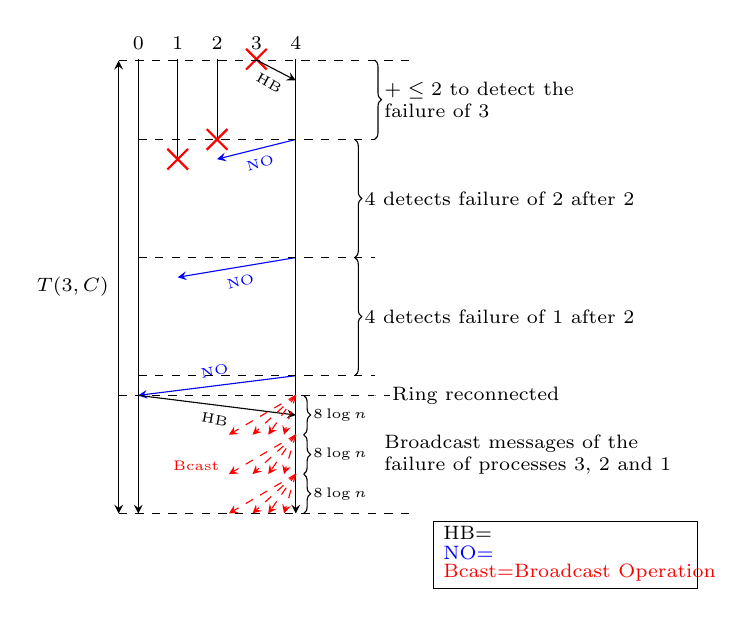
\begin{tikzpicture}
%%%%% position of the first process and distance between processes
%\begin{minipage}[t]{0.5\textwidth}
\def\z{0}
\def\s{0.5}
%%%%% lenght of the execution
\def\l{6}
%%%%% delta duration
\def\Tau{0.25}
\def\Delta{0.75}
%%%failure begin coordinate
\def\fb{0.01}
%%%failure end coordinate
\def\fe{0.50}
%%%% dashed lines for delta
\def\f{0.3}
%%%% number of faults
\def\nbf{3}
\def\propag{0.50}
\pgfmathsetmacro{\nbfmo}{\nbf - 1};
%%%%% beginning of reconnection tentative
\pgfmathsetmacro{\detect}{2 * \Delta}
\def\BeginRec{\l - \fb -\fb - \Tau - \Delta}
\def\Failure3{\BeginRec - \Tau - \Delta - \detect}
\def\BeginBcast{ \BeginRec - \nbfmo * \detect - \Tau}
\def\EndRec{\BeginBcast - \nbfmo * \propag - \propag}
%\foreach \x \in {1, 2, 4}
%{

%}
%%   \draw [>=stealth,->] (\z + 4*\s,\l) -- (\z + 4*\s, \EndRec);
%%   \node at (\z + 4 * \s,\l) [font=\scriptsize,above]{$5$};

  \draw [>=stealth,->] (\z - \s,\l) -- (\z - \s, \EndRec);
  \node at (\z - \s,\l) [font=\scriptsize,above]{$0$};

  \draw [>=stealth,->] (\z + 3*\s,\l) -- (\z + 3*\s, \EndRec);
  \node at (\z + 3*\s,\l) [font=\scriptsize,above]{$4$};
%%% nodes
  \draw (\z + 2 *\s,\l) -- (\z + 2 * \s, \l) node [cross out, draw, red,
  thick]{};
%  \node at (\z,\l) [font=\scriptsize,above]{$1$};
%\draw (\z + \s,\l) -- (\z + \s, \BeginRec - \Tau - \detect - \Tau - \fb )node [cross out, draw, red,
  \draw (\z + \s,\l) -- (\z +\s, \BeginRec) node [cross out, draw, red,
  thick]{};
\node at (\z + \s,\l) [font=\scriptsize,above]{$2$};
\draw (\z,\l) -- (\z,  \BeginRec - \Tau) node [cross out, draw, red,
  thick]{};;
\node at (\z,\l) [font=\scriptsize,above]{$1$};

%\draw (\z, \l) -- (\z, \l - \fb - \fb) node [cross out, draw, red,
%  thick]{};
\node at (\z + 2 * \s, \l) [font=\scriptsize,above]{$3$};


%%%% heartbeat
\draw  [>=stealth,->] (\z + 2*\s, \l - \fb) -- (\z+3*\s, \l - \fb - \fb - \Tau ) node [font=\tiny,midway,rotate=331,below]{HB};
%%% explanation for failure detection
\draw [decoration={brace}, decorate] (\z + 4*\s + 0.5,\l - \fb) -- (\z + 4*\s + 0.5,\BeginRec) node [black,midway,
  right,font=\scriptsize,align=left]{$\msgtime + \suspectinterval \leq 2 \suspectinterval$ to detect the \\ failure of $3$};


%%%%% Failures detection of 2 delimitation
%\draw[dashed](\z -\s, \BeginRec - \Tau - \Delta) -- (\z + 5*\s,  \BeginRec - \Tau - \Delta);
%\draw [decoration={brace}, decorate] (\z + 4*\s + 0.25, \BeginRec) -- (\z + 4*\s + 0.25,\BeginRec - \Tau - \Delta) node [black,midway,
%  right,font=\tiny,align=left]{$3$ detects failure of $2$ after $R(1)$\\ This failure increases the size \\ of the segment $I_1=\{1\}$ by one};



%%%% 4 detects 3's failure
%\draw [decoration={brace}, decorate] (\z + 4*\s + 0.25, \Failure3) -- (\z + 4*\s + 0.25,\Failure3 - \Tau - \Delta) node [black,midway,
%  right,font=\tiny,align=left]{$4$ detects failure of $3$ after $R(1)$\\ This failure increases the size of \\ the segment $I_1=\{1,2\}$ by one};


%%%% 4's reconnection messages
\foreach \x in {2,1,0}
{
  \pgfmathtruncatemacro{\y}{2 - \x};
  \pgfmathtruncatemacro{\i}{\x - 1};
  \ifthenelse{\NOT \x = 0}
             {\draw [>=stealth,->,blue] (\z + 3 * \s, \BeginRec - \y * \detect) -- (\z + \i * \s, \BeginRec - \Tau - \y * \detect) node [font=\tiny,midway,rotate=15,below]{NO};}
             {\draw [>=stealth,->,blue] (\z + 3 * \s, \BeginRec - \y * \detect) -- (\z + \i * \s, \BeginRec - \Tau - \y * \detect) node [font=\tiny,midway,rotate=10,above]{NO};}
  \draw[dashed](\z -\s, \BeginRec - \y * \detect) -- (\z + 5*\s,  \BeginRec - \y * \detect);
\ifthenelse{\NOT \x = 0}{
\ifthenelse{\x = 2}{
  \draw [decoration={brace}, decorate] (\z + 4*\s + 0.25, \BeginRec - \y * \detect) -- (\z + 4*\s + 0.25,\BeginRec - \y * \detect - \detect) node [black,midway,
 right,font=\scriptsize,align=left]{$4$ detects failure of $\x$ after $2\suspectinterval$};}
{
  \draw [decoration={brace}, decorate] (\z + 4*\s + 0.25, \BeginRec - \y * \detect) -- (\z + 4*\s + 0.25,\BeginRec - \y * \detect - \detect) node [black,midway,
 right,font=\scriptsize,align=left]{$4$ detects failure of $\x$ after $2\suspectinterval$};}
}
{
\draw [dashed] (-0.75, \BeginRec - \nbfmo * \detect - \Tau) -- (\z + 5 * \s + 0.20, \BeginRec - \nbfmo * \detect - \Tau);
\draw (\z + 5*\s + 0.10, \BeginRec - \nbfmo * \detect - \Tau) node [font=\scriptsize,right]{Ring reconnected};
%%%heartbeat of the healthy process
\draw  [>=stealth,->] (\z-\s, \BeginRec - \nbfmo * \detect - \Tau) -- (\z + 3*\s,  \BeginRec - \nbfmo * \detect - \Tau - \Tau) node [font=\tiny,midway,rotate=350,below]{HB};
}
}


%%%% Broadcast begin
\foreach \x in {1,...,\nbf}
{
  \pgfmathtruncatemacro{\y}{\x - 1};
  \pgfmathtruncatemacro{\p}{4 - \x};
\foreach \q in {1, 2, 3}
{
  \draw [dashed,red,>=stealth,->] (\z + 3*\s,\BeginBcast - \y * \propag) -- (\z + 1.5 *\s + 0.2*\q,\BeginBcast - \y * \propag - \propag);
}

%\ifthenelse{\x = 2}
%{  \draw [dashed,red,>=stealth,->] (\z + 3*\s,\BeginBcast - \y * \propag) -- (\z + 1.3 *\s,\BeginBcast - \y * \propag - \propag);
 \draw [dashed,red,>=stealth,->] (\z + 3*\s,\BeginBcast - \y * \propag) -- (\z + 1.3 *\s,\BeginBcast - \y * \propag - \propag);
  \draw [decoration={brace}, decorate] (\z + 3 *\s + 0.10,\BeginBcast - \y * \propag) -- (\z + 3*\s + 0.10,\BeginBcast - \propag - \y * \propag) node [black,midway,
  right,font=\tiny,align=left]{$8 \msgtime \log n$};
}

\draw node at (\z + 1.3 *\s,\BeginBcast -  \propag - \propag  + 0.10) [font=\tiny,left,red]{Bcast};

\draw [decoration={brace}, decorate,white] (\z + 3 *\s + 1,\BeginBcast) -- (\z + 3*\s + 1,\BeginBcast -  \nbf * \propag) node [black,midway,
  right,font=\scriptsize,align=left]{Broadcast messages of the \\ failure of processes $3$, $2$ and $1$};

%%% T(3)
\draw [dashed] (-0.75, \l - \fb - \fb) -- (3, \l - \fb - \fb);
\draw [dashed] (-0.75, \EndRec) -- (3, \EndRec);
\draw [>=stealth,<->] (-0.75, \l - \fb - \fb) -- (-0.75, \EndRec) node [font=\scriptsize,left,midway]{$T(\nbf,C)$};

\draw (3.25, \EndRec - 0.10) rectangle (6.60,\EndRec - 0.65 - 0.10 - 0.20);
\draw node at (3.25, \EndRec - 0.10 - 0.15) [font=\scriptsize,right]{HB=\heartbeat};
\draw node at (3.25, \EndRec - 0.10 - 0.40) [font=\scriptsize,right,blue]{NO=\newobserver};
\draw node at (3.25, \EndRec - 0.10 - 0.65) [font=\scriptsize,right,red]{Bcast=Broadcast Operation};

%\draw[dashed](0, \l - \fb) -- (5, \l - \fb);

%% \foreach \x in {1,3}
%% {
%%   \pgfmathtruncatemacro{\y}{3 - \x};
%%   \draw[dashed](\z -\s, \BeginRec - \y * \detect - \y * \Tau) -- (\z + 5*\s,  \BeginRec - \y * \detect - \y * \Tau);
%% }
%% \draw[dashed](\z -\s, \BeginRec - 3 * \detect - 2 * \Tau) -- (\z + 5*\s,  \BeginRec - 3 * \detect - 2 * \Tau);

\end{tikzpicture}
}
\end{column}
\end{columns}
\end{frame}

\begin{frame}
\frametitle{Noise}
\hspace*{-0.5cm}
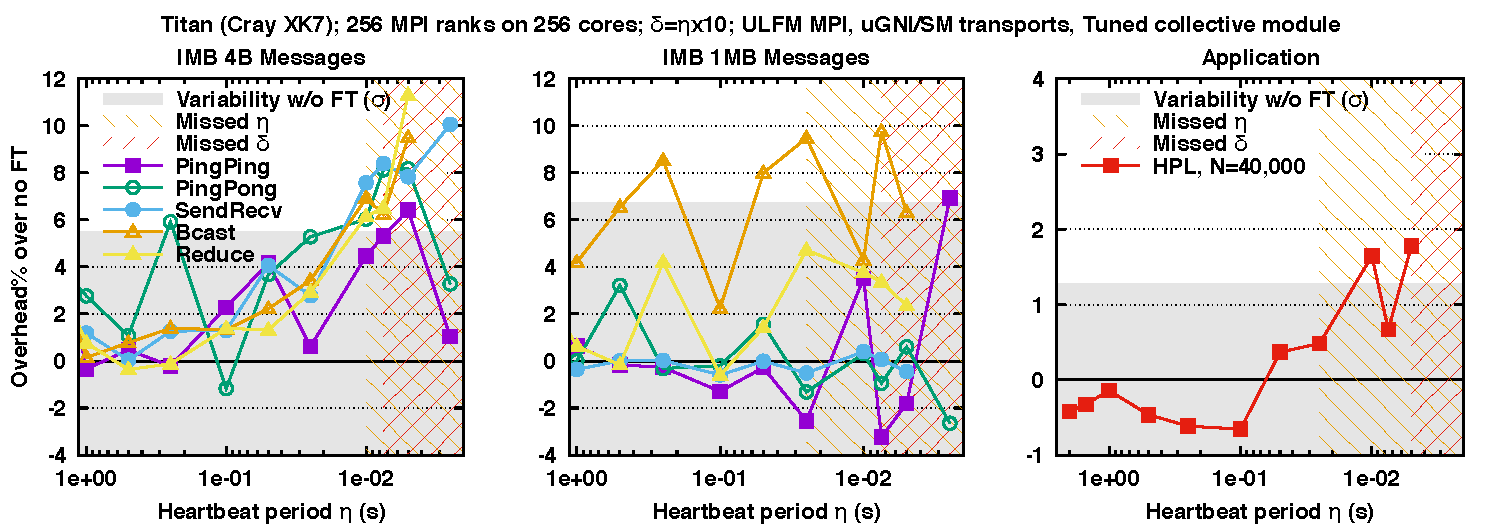
\includegraphics[width=1.1\textwidth]{etanoise-titan.pdf}
\end{frame}

\begin{frame}
\frametitle{Detection and propagation delay}
\hspace*{-0.5cm}
\includegraphics[width=1.1\textwidth]{recva-titan.pdf}
\end{frame}


\subsection{Early Returning Agreement}

\pgfdeclarelayer{background}
\pgfdeclarelayer{foreground}
\pgfsetlayers{background,main,foreground}

\newcommand{\pie}[1]{%
\begin{tikzpicture}
 \draw (0,0) circle (.3em);\fill (.3em,0) arc (0:#1:.3em) -- (0,0) -- cycle;
\end{tikzpicture}%
}

\def\stateUP{\textcolor{black}{\ensuremath{\uparrow}}}
\def\stateDOWN{\textcolor{black}{\ensuremath{\downarrow}}}
\def\stateNOTPART{\textcolor{black}{\ensuremath{?}}}
\def\stateDECIDED{\textcolor{black}{\ensuremath{\pie{360}}}}

\def\msgPART{\textcolor{blue!75}{\ensuremath{\pie{180}}}}
\def\msgDECIDE{\textcolor{blue!75}{\ensuremath{\pie{360}}}}
\def\msgRR{\textcolor{blue!75}{\textbf{?}}}

\renewcommand{\proc}[2]{\expandafter\gdef\csname proc:#1:style\endcsname{alivenode}
\ifcase#2
% Case 0
\expandafter\gdef\csname proc:#1:label\endcsname{\stateUP}
\or
% Case 1
\expandafter\gdef\csname proc:#1:label\endcsname{\stateDOWN}
\or
% Case 2
\expandafter\gdef\csname proc:#1:label\endcsname{\stateNOTPART}
\or
% Case 3
\expandafter\gdef\csname proc:#1:label\endcsname{\ensuremath{#1}}
\or
% Case 4
\expandafter\gdef\csname proc:#1:label\endcsname{\stateDECIDED}
\or
%Case 5
\expandafter\gdef\csname proc:#1:label\endcsname{}
\expandafter\gdef\csname proc:#1:style\endcsname{deadnode}
\fi}
\newcommand{\state}[1]{\foreach \x [count=\xi] in {#1} {\proc{\xi}{\x}}}
\newcommand{\proclabel}[1]{\csname proc:#1:label\endcsname\relax}
\newcommand{\procstyle}[1]{\csname proc:#1:style\endcsname\relax}
\tikzstyle{alivenode} = [draw,shape=circle,minimum size=.75cm,inner sep=0pt,fill=blue!20]
\tikzstyle{deadnode} = [draw,shape=circle,minimum size=.75cm,inner sep=0pt,fill=blue!5,text=blue!5,draw=black!10]
\tikzstyle{aliveedge} = [draw=black,line width=1]
\tikzstyle{deadedge} = [draw=black!10,line width=1]
\newcommand{\msgtype}[1]{\ifcase#1
% Case 0
\ensuremath{\msgPART}
\or
% Case 1
\ensuremath{\msgDECIDE}
\or
% Case 2
\msgRR
\fi}
\def\msg#1#2#3{\path[->] (P#1) edge[blue!75,bend right=30,pos=.5] node[draw=blue!75,fill=white,inner sep=2pt,scale=0.5] {\msgtype{#3}} (P#2);}
\def\monitor#1#2{\pgfmathanglebetweenpoints{\pgfpointanchor{P#1}{center}}{\pgfpointanchor{P#2}{center}}%
\pgfmathsetmacro{\angle}{\pgfmathresult - 90}%
\path[] (P#1) edge[near start] node[rotate=\angle] {\includegraphics[width=.35cm]{FD.png}} (P#2);}
\def\monitoring{\includegraphics[width=.35cm,angle=270,origin=c]{FD.png}}


\begin{frame}
  \frametitle{Consensus in the context of HPC}

  Consider the case of a broadcast implemented with a binary tree.

      \resizebox{\linewidth}{!}{\begin{tikzpicture}[>=latex',scale=.25]
          \node[draw,alivenode] (root) at (0, 0) {\textcolor{green}{\checked}};
          \node[draw,deadnode] (L) at (-10, -3) {};
          \node[draw,alivenode] (R) at (10, -3) {\textcolor{green}{\checked}};
          \node[draw,alivenode] (LL) at (-15, -6) {\textcolor{red}{$\times$}};
          \node[draw,alivenode] (LR) at (-5, -6) {\textcolor{red}{$\times$}};
          \node[draw,alivenode] (RL) at (5, -6) {\textcolor{green}{\checked}};
          \node[draw,alivenode] (RR) at (15, -6){\textcolor{green}{\checked}};
          \draw (root) edge[->,dashed] (L);
          \draw (root) edge[->] (R);
          \draw (L) edge[->,dashed] (LL);
          \draw (L) edge[->,dashed] (LR);
          \draw (R) edge[->] (RL);
          \draw (R) edge[->] (RR);
        \end{tikzpicture}}

      Failures, that happen during the execution, introduce
      inconsistencies: not all processes know that the broadcast
      operation failed.

      \begin{center}
      Consensus (or agreement) allows to reconcile inconsistent /
      non-uniform states \textcolor{red}{due to failures}.

      It must be \textcolor{green!65!black}{reliable}.

      It must be \textcolor{green!65!black}{efficient}, especially in
      the \textcolor{green!65!black}{failure-free} case.
      \end{center}

\end{frame}

\begin{comment}
\begin{frame}[t]
  \frametitle{ULFM Agreement Specification}

  \texttt{int MPIX\_Comm\_agree(MPI\_Comm comm, int *flag);}\\
  \texttt{MPIX\_COMM\_AGREE(COMM, FLAG, IERROR)}\\
  ~\qquad\qquad\texttt{  INTEGER COMM, FLAG, IERROR}

  \begin{description}
  \item[\texttt{comm}] the communicator on which to apply the
    consensus
  \item[\texttt{flag}] An in/out integer: in input, the process
    participation, in output, the result of the agreement on these
    ints (bitwise and)
  \item[\texttt{return value}] An error code if new process failures
    were discovered during the agreement, or success
  \end{description}
  
  The operation implements an agreement on the couple
  \texttt{(flag, return code)}: all surviving process, despite any 
  failure have the same values in each (even if the return code is an
  error, flag is defined).
 
\end{frame}
\end{comment}

\begin{frame}
  \frametitle{Specification}

  \begin{beamerboxesrounded}{Correctness}
    \begin{description}
    \item[Termination] Every living process eventually decides.
    \item[Integrity] Once a living process decides a value, it remains decided on that value.
    \item[Agreement] No two living processes decide differently.
    \item[Participation] When a process decides upon a value, it
      contributed to the decided value.
    \end{description}
  \end{beamerboxesrounded}

\bigskip

  Traditional consensus relies on \textcolor{green!75!black}{Validity}\\
  This is because \textcolor{red}{one} value is \textcolor{red}{chosen}.

\end{frame}

\begin{frame}
  \frametitle{Assumptions}
  
  \begin{itemize}
  \item Processes have totally ordered, \textcolor{red!75}{unique identifiers}
  \item Any process belonging to a group knows
    \textcolor{blue!75}{what processes belong to that group}
  \item Any process may be subject to a \textcolor{red!75}{permanent failure}
  \item The network does not \textcolor{blue!50!black}{lose},
    \textcolor{red!50!black}{modify}, nor
    \textcolor{green!50!black}{duplicate} messages, but communication
    delays \textcolor{red!75}{have \emph{unknown} bounds}
  \item The system provides a \textcolor{red!50!black}{Perfect Failure
      Detector} (${\mathcal P}$):
    \begin{itemize}
    \item All \textcolor{red!50!black}{incorrect} processes are eventually suspected by all
      \textcolor{green!50!black}{correct} processes
    \item No \textcolor{green!50!black}{correct} process is ever suspected by any process
    \end{itemize}
  \item The operation of the consensus is associative and commutative,
    and idempotent, with a \emph{known neutral element}
  \end{itemize}

\end{frame}


\begin{frame}
  \frametitle{Principle and Notation}
  \begin{columns}[T] % align columns
    \begin{column}{.30\textwidth}
      \begin{center}
      \resizebox{.8\linewidth}{!}{\begin{tikzpicture}[>=latex',scale=.25]
          \node (n) at (0,0) [alivenode] {$$};
          \node (p) at (0,6) {parent};
          \node (lc) at (-6,-6) {left child};
          \node (rc) at (6,-6) {right child};
          \draw (n) edge [aliveedge] (p);
          \draw (n) edge [aliveedge] (lc);
          \draw (n) edge [aliveedge] (rc);
        \end{tikzpicture}}

      \resizebox{.8\linewidth}{!}{\begin{tikzpicture}[>=latex',scale=.25]
          \node (Pn) at (0,0) [alivenode] {\stateUP};
          \node (Pp) at (0,6)  [alivenode] {\stateDOWN};
          \node (Plc) at (-6,-6)  [alivenode] {\stateNOTPART};
          \node (Prc) at (6,-6)  [alivenode] {\stateDECIDED};
          \draw (Pn) edge [aliveedge] (Pp);
          \draw (Pn) edge [aliveedge] (Plc);
          \draw (Pn) edge [aliveedge] (Prc);
          \msg{n}{p}{0}
          \msg{n}{lc}{1}
          \msg{n}{rc}{2}
          \monitor{n}{p}
          \monitor{n}{rc}\monitor{rc}{n}
      \end{tikzpicture}}
      \end{center}
    \end{column}%
    \hfill%
    \begin{column}{.75\textwidth}
\only<1>{
    \begin{itemize}
    \item Processes are arranged following a \textcolor{red}{mendable tree} topology:
      given a list of known dead processes, they communicate or monitor
      the liveliness of only their neighbors in that topology. 
    \item The algorithm is a \textcolor{blue}{resilient version} of Fan-in / Fan-out: all
      contributions (noted \msgPART) are reduced along the tree up to
      the root, that broadcasts it
    \item \emph{Deciding} the result of the consensus for a given
      process consists in \textcolor{red}{remembering} the return value of the
      consensus, \textcolor{blue}{broadcasting} it to the current children, and
      \textcolor{red}{returning} \textit{as if} the consensus was completed.
    \end{itemize}}
\only<2>{
  \footnotesize
  \begin{itemize}
  \item Alive processes can be in 3 states:
    \begin{itemize}
    \item \stateNOTPART, if they have not entered the consensus yet
    \item \stateUP, if they are waiting from the contribution of their
      children
    \item \stateDOWN, if they have sent their contribution to their
      parent and are waiting for the decision
    \item \stateDECIDED, if they have received the decision
    \end{itemize}
  \item There are 3 types of messages:
    \begin{itemize}
    \item \msgPART, when a process sends its participation to a parent
    \item \msgDECIDE, when a process broadcasts the decision to its
      children
    \item \msgRR, when a process enquired about a possible result of
      a completed consensus
    \end{itemize}
  \item Processes can monitor (\monitoring) other processes for failures
  \end{itemize}
}
  \end{column}
  \end{columns}
\end{frame}

\begin{frame}[fragile]
  \frametitle{Mendable Tree for Consensus}

\begin{center}
\resizebox{.45\linewidth}{!}{\begin{tikzpicture}[>=latex',scale=.25]
\proc{1}{3}\proc{2}{3}\proc{3}{3}\proc{4}{3}\proc{5}{3}
\proc{6}{3}\proc{7}{3}\proc{8}{3}\proc{9}{3}\proc{10}{3}
\proc{11}{3}\proc{12}{3}\proc{13}{3}\proc{14}{3}\proc{15}{3}
%%
\node (P2) at (336.0bp,252.5bp) [\procstyle{2}] {$\proclabel{2}$};
  \node (P3) at (494.0bp,252.5bp) [\procstyle{3}] {$\proclabel{3}$};
  \node (P1) at (408.0bp,375.5bp) [\procstyle{1}] {$\proclabel{1}$};
  \node (P6) at (494.0bp,129.5bp) [\procstyle{6}] {$\proclabel{6}$};
  \node (P7) at (666.0bp,129.5bp) [\procstyle{7}] {$\proclabel{7}$};
  \node (P4) at (116.0bp,129.5bp) [\procstyle{4}] {$\proclabel{4}$};
  \node (P5) at (336.0bp,129.5bp) [\procstyle{5}] {$\proclabel{5}$};
  \node (P8) at (6.0bp,6.5bp) [\procstyle{8}] {$\proclabel{8}$};
  \node (P9) at (116.0bp,6.5bp) [\procstyle{9}] {$\proclabel{9}$};
  \node (P10) at (226.0bp,6.5bp) [\procstyle{10}] {$\proclabel{10}$};
  \node (P11) at (336.0bp,6.5bp) [\procstyle{11}] {$\proclabel{11}$};
  \node (P12) at (446.0bp,6.5bp) [\procstyle{12}] {$\proclabel{12}$};
  \node (P13) at (556.0bp,6.5bp) [\procstyle{13}] {$\proclabel{13}$};
  \node (P14) at (666.0bp,6.5bp) [\procstyle{14}] {$\proclabel{14}$};
  \node (P15) at (776.0bp,6.5bp) [\procstyle{15}] {$\proclabel{15}$};
%
  \draw [aliveedge] (P4) -- node {$$} (P9);
  \draw [aliveedge] (P4) -- node {$$} (P8);
  \draw [aliveedge] (P6) -- node {$$} (P13);
  \draw [aliveedge] (P3) -- node {$$} (P7);
  \draw [aliveedge] (P1) -- node {$$} (P2);
  \draw [aliveedge] (P6) -- node {$$} (P12);
  \draw [aliveedge] (P1) -- node {$$} (P3);
  \draw [aliveedge] (P3) -- node {$$} (P6);
  \draw [aliveedge] (P2) -- node {$$} (P4);
  \draw [aliveedge] (P7) -- node {$$} (P14);
  \draw [aliveedge] (P5) -- node {$$} (P10);
  \draw [aliveedge] (P2) -- node {$$} (P5);
  \draw [aliveedge] (P5) -- node {$$} (P11);
  \draw [aliveedge] (P7) -- node {$$} (P15);
\end{tikzpicture}}
\hspace{\stretch{1}}
\only<1>{\resizebox{.45\linewidth}{!}{\begin{tikzpicture}[>=latex',scale=.25]
\proc{1}{3}\proc{2}{3}\proc{3}{5}\proc{4}{3}\proc{5}{3}
\proc{6}{5}\proc{7}{3}\proc{8}{3}\proc{9}{3}\proc{10}{3}
\proc{11}{3}\proc{12}{3}\proc{13}{5}\proc{14}{3}\proc{15}{3}
%%
\node (P2) at (336.0bp,252.5bp) [\procstyle{2}] {$\proclabel{2}$};
  \node (P3) at (494.0bp,252.5bp) [\procstyle{3}] {$\proclabel{3}$};
  \node (P1) at (408.0bp,375.5bp) [\procstyle{1}] {$\proclabel{1}$};
  \node (P6) at (494.0bp,129.5bp) [\procstyle{6}] {$\proclabel{6}$};
  \node (P7) at (666.0bp,129.5bp) [\procstyle{7}] {$\proclabel{7}$};
  \node (P4) at (116.0bp,129.5bp) [\procstyle{4}] {$\proclabel{4}$};
  \node (P5) at (336.0bp,129.5bp) [\procstyle{5}] {$\proclabel{5}$};
  \node (P8) at (6.0bp,6.5bp) [\procstyle{8}] {$\proclabel{8}$};
  \node (P9) at (116.0bp,6.5bp) [\procstyle{9}] {$\proclabel{9}$};
  \node (P10) at (226.0bp,6.5bp) [\procstyle{10}] {$\proclabel{10}$};
  \node (P11) at (336.0bp,6.5bp) [\procstyle{11}] {$\proclabel{11}$};
  \node (P12) at (446.0bp,6.5bp) [\procstyle{12}] {$\proclabel{12}$};
  \node (P13) at (556.0bp,6.5bp) [\procstyle{13}] {$\proclabel{13}$};
  \node (P14) at (666.0bp,6.5bp) [\procstyle{14}] {$\proclabel{14}$};
  \node (P15) at (776.0bp,6.5bp) [\procstyle{15}] {$\proclabel{15}$};
%
  \draw [aliveedge] (P1) -- node {$$} (P2);
  % \draw [aliveedge] (P1) -- node {$$} (P3);
  \draw [aliveedge] (P2) -- node {$$} (P4);
  \draw [aliveedge] (P2) -- node {$$} (P5);
  % \draw [aliveedge] (P3) -- node {$$} (P7);
  % \draw [aliveedge] (P3) -- node {$$} (P6);
  \draw [aliveedge] (P4) -- node {$$} (P8);
  \draw [aliveedge] (P4) -- node {$$} (P9);
  \draw [aliveedge] (P5) -- node {$$} (P10);
  \draw [aliveedge] (P5) -- node {$$} (P11);
  % \draw [aliveedge] (P6) -- node {$$} (P13);
  % \draw [aliveedge] (P6) -- node {$$} (P12);
  \draw [aliveedge] (P7) -- node {$$} (P14);
  \draw [aliveedge] (P7) -- node {$$} (P15);
  \draw [aliveedge] (P12) -- node {$$} (P1);
  \draw [aliveedge] (P7) -- node {$$} (P1);
\end{tikzpicture}}}
\only<2>{\resizebox{.45\linewidth}{!}{\begin{tikzpicture}[>=latex',scale=.25]
\proc{1}{5}\proc{2}{5}\proc{3}{3}\proc{4}{3}\proc{5}{3}
\proc{6}{3}\proc{7}{3}\proc{8}{3}\proc{9}{3}\proc{10}{3}
\proc{11}{3}\proc{12}{3}\proc{13}{3}\proc{14}{3}\proc{15}{3}
%%
\node (P2) at (336.0bp,252.5bp) [\procstyle{2}] {$\proclabel{2}$};
  \node (P3) at (494.0bp,252.5bp) [\procstyle{3}] {$\proclabel{3}$};
  \node (P1) at (408.0bp,375.5bp) [\procstyle{1}] {$\proclabel{1}$};
  \node (P6) at (494.0bp,129.5bp) [\procstyle{6}] {$\proclabel{6}$};
  \node (P7) at (666.0bp,129.5bp) [\procstyle{7}] {$\proclabel{7}$};
  \node (P4) at (116.0bp,129.5bp) [\procstyle{4}] {$\proclabel{4}$};
  \node (P5) at (336.0bp,129.5bp) [\procstyle{5}] {$\proclabel{5}$};
  \node (P8) at (6.0bp,6.5bp) [\procstyle{8}] {$\proclabel{8}$};
  \node (P9) at (116.0bp,6.5bp) [\procstyle{9}] {$\proclabel{9}$};
  \node (P10) at (226.0bp,6.5bp) [\procstyle{10}] {$\proclabel{10}$};
  \node (P11) at (336.0bp,6.5bp) [\procstyle{11}] {$\proclabel{11}$};
  \node (P12) at (446.0bp,6.5bp) [\procstyle{12}] {$\proclabel{12}$};
  \node (P13) at (556.0bp,6.5bp) [\procstyle{13}] {$\proclabel{13}$};
  \node (P14) at (666.0bp,6.5bp) [\procstyle{14}] {$\proclabel{14}$};
  \node (P15) at (776.0bp,6.5bp) [\procstyle{15}] {$\proclabel{15}$};
%
%  \draw [aliveedge] (P1) -- node {$$} (P2);
%  \draw [aliveedge] (P1) -- node {$$} (P3);
%  \draw [aliveedge] (P2) -- node {$$} (P4);
%  \draw [aliveedge] (P2) -- node {$$} (P5);
  \draw [aliveedge] (P3) -- node {$$} (P4);
  \draw [aliveedge] (P3) -- node {$$} (P5);
  \draw [aliveedge] (P3) -- node {$$} (P7);
  \draw [aliveedge] (P3) -- node {$$} (P6);
  \draw [aliveedge] (P4) -- node {$$} (P8);
  \draw [aliveedge] (P4) -- node {$$} (P9);
  \draw [aliveedge] (P5) -- node {$$} (P10);
  \draw [aliveedge] (P5) -- node {$$} (P11);
  \draw [aliveedge] (P6) -- node {$$} (P13);
  \draw [aliveedge] (P6) -- node {$$} (P12);
  \draw [aliveedge] (P7) -- node {$$} (P14);
  \draw [aliveedge] (P7) -- node {$$} (P15);
\end{tikzpicture}}}
\only<3>{\resizebox{.45\linewidth}{!}{\begin{tikzpicture}[>=latex',scale=.25]
\proc{1}{5}\proc{2}{5}\proc{3}{5}\proc{4}{5}\proc{5}{5}
\proc{6}{5}\proc{7}{5}\proc{8}{3}\proc{9}{3}\proc{10}{3}
\proc{11}{3}\proc{12}{3}\proc{13}{3}\proc{14}{3}\proc{15}{3}
%%
\node (P2) at (336.0bp,252.5bp) [\procstyle{2}] {$\proclabel{2}$};
  \node (P3) at (494.0bp,252.5bp) [\procstyle{3}] {$\proclabel{3}$};
  \node (P1) at (408.0bp,375.5bp) [\procstyle{1}] {$\proclabel{1}$};
  \node (P6) at (494.0bp,129.5bp) [\procstyle{6}] {$\proclabel{6}$};
  \node (P7) at (666.0bp,129.5bp) [\procstyle{7}] {$\proclabel{7}$};
  \node (P4) at (116.0bp,129.5bp) [\procstyle{4}] {$\proclabel{4}$};
  \node (P5) at (336.0bp,129.5bp) [\procstyle{5}] {$\proclabel{5}$};
  \node (P8) at (6.0bp,6.5bp) [\procstyle{8}] {$\proclabel{8}$};
  \node (P9) at (116.0bp,6.5bp) [\procstyle{9}] {$\proclabel{9}$};
  \node (P10) at (226.0bp,6.5bp) [\procstyle{10}] {$\proclabel{10}$};
  \node (P11) at (336.0bp,6.5bp) [\procstyle{11}] {$\proclabel{11}$};
  \node (P12) at (446.0bp,6.5bp) [\procstyle{12}] {$\proclabel{12}$};
  \node (P13) at (556.0bp,6.5bp) [\procstyle{13}] {$\proclabel{13}$};
  \node (P14) at (666.0bp,6.5bp) [\procstyle{14}] {$\proclabel{14}$};
  \node (P15) at (776.0bp,6.5bp) [\procstyle{15}] {$\proclabel{15}$};
%
  \draw [aliveedge] (P8) edge[bend left=10] node {$$} (P9);
  \draw [aliveedge] (P8) edge[bend right=10] node {$$} (P10);
  \draw [aliveedge] (P8) edge[bend left=15] node {$$} (P11);
  \draw [aliveedge] (P8) edge[bend right=15] node {$$} (P12);
  \draw [aliveedge] (P8) edge[bend left=20] node {$$} (P13);
  \draw [aliveedge] (P8) edge[bend right=20] node {$$} (P14);
  \draw [aliveedge] (P8) edge[bend left=25] node {$$} (P15);
\end{tikzpicture}}}
\end{center}

\only<1>{ The Fan-in Fan-out tree used during the consensus is
  \textcolor{green!75}{mended}, as failures are discovered during the
  execution.

  The mending rule is simple: processes are arranged according to
  their (MPI) rank following a \textcolor{red!75}{breath-first} search
  of the tree}

\only<2>{ Nodes replace their parents by the
  \textcolor{red!75}{highest-ranked alive ancester} in the tree in
  case of failure.
  
  Processes without an alive ancestor in the original tree connect to
  the \textcolor{red!75}{lowest alive processor} as their
  parent. \emph{The lowest alive processor is always the root of the
    tree} }

\only<3>{If half the processes die, the tree can, in the worst case,
  degenerate to a \textcolor{blue!75}{$np/2$-degree star}}

\end{frame}

\begin{frame}[fragile]
  \frametitle{Architecture-Aware Tree}

  \begin{center}
    \resizebox{\linewidth}{!}{\begin{tikzpicture}[>=latex',scale=.25]
          \node (P3_9) at (1619.0bp,164.0bp) [alivenode] {$$};
  \node (P1_a) at (1015.0bp,310.0bp) [alivenode] {$$};
  \node (P3_8) at (1509.0bp,164.0bp) [alivenode] {$$};
  \node (P1_0) at (1086.0bp,748.0bp) [alivenode] {$$};
  \node (P1_1) at (1017.0bp,602.0bp) [alivenode] {$$};
  \node (P1_2) at (1154.0bp,602.0bp) [alivenode] {$$};
  \node (P1_3) at (905.0bp,456.0bp) [alivenode] {$$};
  \node (P1_4) at (1015.0bp,456.0bp) [alivenode] {$$};
  \node (P1_5) at (1154.0bp,456.0bp) [alivenode] {$$};
  \node (P1_6) at (1345.0bp,456.0bp) [alivenode] {$$};
  \node (P1_7) at (685.0bp,310.0bp) [alivenode] {$$};
  \node (P0_1) at (302.0bp,748.0bp) [alivenode] {$$};
  \node (P1_9) at (905.0bp,310.0bp) [alivenode] {$$};
  \node (P0_3) at (137.0bp,602.0bp) [alivenode] {$$};
  \node (P0_2) at (769.0bp,748.0bp) [alivenode] {$$};
  \node (P0_5) at (577.0bp,602.0bp) [alivenode] {$$};
  \node (P0_4) at (302.0bp,602.0bp) [alivenode] {$$};
  \node (P0_7) at (27.0bp,456.0bp) [alivenode] {$$};
  \node (P0_6) at (769.0bp,602.0bp) [alivenode] {$$};
  \node (P3_6) at (2059.0bp,310.0bp) [alivenode] {$$};
  \node (P3_7) at (1399.0bp,164.0bp) [alivenode] {$$};
  \node (P3_4) at (1675.0bp,310.0bp) [alivenode] {$$};
  \node (P3_5) at (1892.0bp,310.0bp) [alivenode] {$$};
  \node (P3_2) at (1892.0bp,456.0bp) [alivenode] {$$};
  \node (P3_3) at (1563.0bp,310.0bp) [alivenode] {$$};
  \node (P3_0) at (1620.0bp,602.0bp) [alivenode] {$$};
  \node (P3_1) at (1620.0bp,456.0bp) [alivenode] {$$};
  \node (P2_7) at (2223.0bp,310.0bp) [alivenode] {$$};
  \node (P2_6) at (2882.0bp,456.0bp) [alivenode] {$$};
  \node (P2_5) at (2717.0bp,456.0bp) [alivenode] {$$};
  \node (P2_4) at (2442.0bp,456.0bp) [alivenode] {$$};
  \node (P2_3) at (2332.0bp,456.0bp) [alivenode] {$$};
  \node (P2_2) at (2717.0bp,602.0bp) [alivenode] {$$};
  \node (P2_1) at (2387.0bp,602.0bp) [alivenode] {$$};
  \node (P2_0) at (2387.0bp,748.0bp) [alivenode] {$$};
  \node (P0_9) at (247.0bp,456.0bp) [alivenode] {$$};
  \node (P2_9) at (2442.0bp,310.0bp) [alivenode] {$$};
  \node (P0_8) at (137.0bp,456.0bp) [alivenode] {$$};
  \node (P2_8) at (2332.0bp,310.0bp) [alivenode] {$$};
  \node (P3_f) at (1399.0bp,18.0bp) [alivenode] {$$};
  \node (P3_d) at (2059.0bp,164.0bp) [alivenode] {$$};
  \node (P3_e) at (2169.0bp,164.0bp) [alivenode] {$$};
  \node (P3_b) at (1839.0bp,164.0bp) [alivenode] {$$};
  \node (P3_c) at (1949.0bp,164.0bp) [alivenode] {$$};
  \node (P3_a) at (1729.0bp,164.0bp) [alivenode] {$$};
  \node (P2_f) at (2279.0bp,164.0bp) [alivenode] {$$};
  \node (P2_e) at (2992.0bp,310.0bp) [alivenode] {$$};
  \node (P2_d) at (2882.0bp,310.0bp) [alivenode] {$$};
  \node (P2_c) at (2772.0bp,310.0bp) [alivenode] {$$};
  \node (P2_b) at (2662.0bp,310.0bp) [alivenode] {$$};
  \node (P2_a) at (2552.0bp,310.0bp) [alivenode] {$$};
  \node (P1_8) at (795.0bp,310.0bp) [alivenode] {$$};
  \node (P1_b) at (1125.0bp,310.0bp) [alivenode] {$$};
  \node (P1_c) at (1235.0bp,310.0bp) [alivenode] {$$};
  \node (P1_d) at (1345.0bp,310.0bp) [alivenode] {$$};
  \node (P1_e) at (1455.0bp,310.0bp) [alivenode] {$$};
  \node (P1_f) at (685.0bp,164.0bp) [alivenode] {$$};
  \node (P0_0) at (879.0bp,894.0bp) [alivenode] {$$};
  \node (P0_a) at (357.0bp,456.0bp) [alivenode] {$$};
  \node (P0_c) at (577.0bp,456.0bp) [alivenode] {$$};
  \node (P0_b) at (467.0bp,456.0bp) [alivenode] {$$};
  \node (P0_e) at (797.0bp,456.0bp) [alivenode] {$$};
  \node (P0_d) at (687.0bp,456.0bp) [alivenode] {$$};
  \node (P0_f) at (27.0bp,310.0bp) [alivenode] {$$};
  \draw [aliveedge] (P1_0) -- node {$$} (P3_0);
  \draw [aliveedge] (P1_2) -- node {$$} (P1_6);
  \draw [aliveedge] (P0_1) -- node {$$} (P0_4);
  \draw [aliveedge] (P3_2) -- node {$$} (P3_5);
  \draw [aliveedge] (P0_4) -- node {$$} (P0_a);
  \draw [aliveedge] (P0_0) -- node {$$} (P0_1);
  \draw [aliveedge] (P3_6) -- node {$$} (P3_d);
  \draw [aliveedge] (P1_1) -- node {$$} (P1_4);
  \draw [aliveedge] (P1_5) -- node {$$} (P1_c);
  \draw [aliveedge] (P3_1) -- node {$$} (P3_3);
  \draw [aliveedge] (P2_0) -- node {$$} (P2_2);
  \draw [aliveedge] (P2_2) -- node {$$} (P2_6);
  \draw [aliveedge] (P1_7) -- node {$$} (P1_f);
  \draw [aliveedge] (P2_4) -- node {$$} (P2_9);
  \draw [aliveedge] (P2_3) -- node {$$} (P2_7);
  \draw [aliveedge] (P1_0) -- node {$$} (P1_1);
  \draw [aliveedge] (P3_0) -- node {$$} (P3_2);
  \draw [aliveedge] (P0_0) -- node {$$} (P1_0);
  \draw [aliveedge] (P3_0) -- node {$$} (P3_1);
  \draw [aliveedge] (P0_7) -- node {$$} (P0_f);
  \draw [aliveedge] (P3_4) -- node {$$} (P3_a);
  \draw [aliveedge] (P2_4) -- node {$$} (P2_a);
  \draw [aliveedge] (P2_1) -- node {$$} (P2_3);
  \draw [aliveedge] (P0_5) -- node {$$} (P0_c);
  \draw [aliveedge] (P3_6) -- node {$$} (P3_e);
  \draw [aliveedge] (P1_5) -- node {$$} (P1_b);
  \draw [aliveedge] (P0_1) -- node {$$} (P0_3);
  \draw [aliveedge] (P3_5) -- node {$$} (P3_c);
  \draw [aliveedge] (P1_3) -- node {$$} (P1_8);
  \draw [aliveedge] (P0_0) -- node {$$} (P0_2);
  \draw [aliveedge] (P2_0) -- node {$$} (P2_1);
  \draw [aliveedge] (P1_0) -- node {$$} (P1_2);
  \draw [aliveedge] (P2_6) -- node {$$} (P2_e);
  \draw [aliveedge] (P1_1) -- node {$$} (P1_3);
  \draw [aliveedge] (P0_5) -- node {$$} (P0_b);
  \draw [aliveedge] (P3_5) -- node {$$} (P3_b);
  \draw [aliveedge] (P2_6) -- node {$$} (P2_d);
  \draw [aliveedge] (P3_3) -- node {$$} (P3_7);
  \draw [aliveedge] (P3_3) -- node {$$} (P3_8);
  \draw [aliveedge] (P0_6) -- node {$$} (P0_d);
  \draw [aliveedge] (P1_6) -- node {$$} (P1_e);
  \draw [aliveedge] (P0_3) -- node {$$} (P0_8);
  \draw [aliveedge] (P0_0) -- node {$$} (P2_0);
  \draw [aliveedge] (P2_5) -- node {$$} (P2_c);
  \draw [aliveedge] (P1_3) -- node {$$} (P1_7);
  \draw [aliveedge] (P1_2) -- node {$$} (P1_5);
  \draw [aliveedge] (P2_7) -- node {$$} (P2_f);
  \draw [aliveedge] (P0_2) -- node {$$} (P0_5);
  \draw [aliveedge] (P2_1) -- node {$$} (P2_4);
  \draw [aliveedge] (P1_4) -- node {$$} (P1_9);
  \draw [aliveedge] (P2_3) -- node {$$} (P2_8);
  \draw [aliveedge] (P1_4) -- node {$$} (P1_a);
  \draw [aliveedge] (P2_5) -- node {$$} (P2_b);
  \draw [aliveedge] (P0_6) -- node {$$} (P0_e);
  \draw [aliveedge] (P1_6) -- node {$$} (P1_d);
  \draw [aliveedge] (P0_3) -- node {$$} (P0_7);
  \draw [aliveedge] (P3_1) -- node {$$} (P3_4);
  \draw [aliveedge] (P3_4) -- node {$$} (P3_9);
  \draw [aliveedge] (P0_2) -- node {$$} (P0_6);
  \draw [aliveedge] (P2_2) -- node {$$} (P2_5);
  \draw [aliveedge] (P3_7) -- node {$$} (P3_f);
  \draw [aliveedge] (P0_4) -- node {$$} (P0_9);
  \draw [aliveedge] (P3_2) -- node {$$} (P3_6);
        \begin{pgfonlayer}{background}
%node 0
          \draw[rounded corners=2em,line width=3em,red!20,cap=round]
          (P0_0.center) -- (P0_1.center) -- (P0_3.center) -- (P0_7.center)  -- (P0_f.center);
          \draw[rounded corners=2em,line width=3em,red!20,cap=round]
          (P0_0.center) -- (P0_2.center) -- (P0_5.center) --
          (P0_b.center);
          \draw[rounded corners=2em,line width=3em,red!20,cap=round]
          (P0_1.center) -- (P0_4.center) -- (P0_9.center);
          \draw[rounded corners=2em,line width=3em,red!20,cap=round]
          (P0_4.center) -- (P0_a.center);
          \draw[rounded corners=2em,line width=3em,red!20,cap=round]
          (P0_2.center) -- (P0_5.center) -- (P0_b.center);
          \draw[rounded corners=2em,line width=3em,red!20,cap=round]
          (P0_5.center) -- (P0_c.center);
          \draw[rounded corners=2em,line width=3em,red!20,cap=round]
          (P0_2.center) -- (P0_6.center) -- (P0_d.center);
          \draw[rounded corners=2em,line width=3em,red!20,cap=round]
          (P0_6.center) -- (P0_e.center);
%node 1
          \draw[rounded corners=2em,line width=3em,green!20,cap=round]
          (P1_0.center) -- (P1_1.center) -- (P1_3.center) -- (P1_7.center)  -- (P1_f.center);
          \draw[rounded corners=2em,line width=3em,green!20,cap=round]
          (P1_0.center) -- (P1_2.center) -- (P1_5.center) --
          (P1_b.center);
          \draw[rounded corners=2em,line width=3em,green!20,cap=round]
          (P1_1.center) -- (P1_4.center) -- (P1_9.center);
          \draw[rounded corners=2em,line width=3em,green!20,cap=round]
          (P1_4.center) -- (P1_a.center);
          \draw[rounded corners=2em,line width=3em,green!20,cap=round]
          (P1_2.center) -- (P1_5.center) -- (P1_b.center);
          \draw[rounded corners=2em,line width=3em,green!20,cap=round]
          (P1_5.center) -- (P1_c.center);
          \draw[rounded corners=2em,line width=3em,green!20,cap=round]
          (P1_2.center) -- (P1_6.center) -- (P1_d.center);
          \draw[rounded corners=2em,line width=3em,green!20,cap=round]
          (P1_6.center) -- (P1_e.center);
%node 2
          \draw[rounded corners=2em,line width=3em,purple!20,cap=round]
          (P2_0.center) -- (P2_1.center) -- (P2_3.center) -- (P2_7.center)  -- (P2_f.center);
          \draw[rounded corners=2em,line width=3em,purple!20,cap=round]
          (P2_0.center) -- (P2_2.center) -- (P2_5.center) --
          (P2_b.center);
          \draw[rounded corners=2em,line width=3em,purple!20,cap=round]
          (P2_1.center) -- (P2_4.center) -- (P2_9.center);
          \draw[rounded corners=2em,line width=3em,purple!20,cap=round]
          (P2_4.center) -- (P2_a.center);
          \draw[rounded corners=2em,line width=3em,purple!20,cap=round]
          (P2_2.center) -- (P2_5.center) -- (P2_b.center);
          \draw[rounded corners=2em,line width=3em,purple!20,cap=round]
          (P2_5.center) -- (P2_c.center);
          \draw[rounded corners=2em,line width=3em,purple!20,cap=round]
          (P2_2.center) -- (P2_6.center) -- (P2_d.center);
          \draw[rounded corners=2em,line width=3em,purple!20,cap=round]
          (P2_6.center) -- (P2_e.center);
%node 3
          \draw[rounded corners=2em,line width=3em,violet!20,cap=round]
          (P3_0.center) -- (P3_1.center) -- (P3_3.center) -- (P3_7.center)  -- (P3_f.center);
          \draw[rounded corners=2em,line width=3em,violet!20,cap=round]
          (P3_0.center) -- (P3_2.center) -- (P3_5.center) --
          (P3_b.center);
          \draw[rounded corners=2em,line width=3em,violet!20,cap=round]
          (P3_1.center) -- (P3_4.center) -- (P3_9.center);
          \draw[rounded corners=2em,line width=3em,violet!20,cap=round]
          (P3_4.center) -- (P3_a.center);
          \draw[rounded corners=2em,line width=3em,violet!20,cap=round]
          (P3_2.center) -- (P3_5.center) -- (P3_b.center);
          \draw[rounded corners=2em,line width=3em,violet!20,cap=round]
          (P3_5.center) -- (P3_c.center);
          \draw[rounded corners=2em,line width=3em,violet!20,cap=round]
          (P3_2.center) -- (P3_6.center) -- (P3_d.center);
          \draw[rounded corners=2em,line width=3em,violet!20,cap=round]
          (P3_6.center) -- (P3_e.center);
        \end{pgfonlayer}

      \end{tikzpicture}}
  \end{center}
  To map the hardware network hierarchy, two levels of trees are
  joined: In the example, \emph{representative} processes of nodes
  (\textcolor{red!20}{node0}, \textcolor{green!20}{node1},
  \textcolor{purple!20}{node2}, \textcolor{violet!20}{node3}) are
  interconnected following a \emph{binary} tree, and processes
  belonging to the same node (16 process / node in this case) are also
  connected following independent \emph{binary} trees.
\end{frame}

\begin{frame}[fragile,t]
  \frametitle{No Failure}

\begin{center}
\begin{tikzpicture}[>=latex',scale=.25]
\only<1>{\state{0,0,0,0,0,0,0,0,0,0,0,0,0,0,0}}
\only<2>{\state{0,0,0,0,0,0,0,1,1,1,1,1,1,1,1}}
\only<3>{\state{0,0,0,1,1,1,1,1,1,1,1,1,1,1,1}}
\only<4>{\state{4,1,1,1,1,1,1,1,1,1,1,1,1,1,1}}
\only<5>{\state{4,1,1,1,1,1,1,1,1,1,1,1,1,1,1}}
\only<6>{\state{4,4,4,1,1,1,1,1,1,1,1,1,1,1,1}}
\only<7>{\state{4,4,4,4,4,4,4,1,1,1,1,1,1,1,1}}
\only<8>{\state{4,4,4,4,4,4,4,4,4,4,4,4,4,4,4}}
\begin{dot2tex}[dot,tikz,codeonly,styleonly,options=-s -tmath,autosize,tikzedgelabels]
graph G {
nodesep=0.75;
node [style="alivenode"];
edge [style="aliveedge",minlen=3];
P1 [label="\proclabel{1}",style="\procstyle{1}"]; P2 [label="\proclabel{2}",style="\procstyle{2}"]; 
P3 [label="\proclabel{3}",style="\procstyle{3}"]; P4 [label="\proclabel{4}",style="\procstyle{4}"]; 
P5 [label="\proclabel{5}",style="\procstyle{5}"]; P6 [label="\proclabel{6}",style="\procstyle{6}"]; 
P7 [label="\proclabel{7}",style="\procstyle{7}"]; P8 [label="\proclabel{8}",style="\procstyle{8}"]; 
P9 [label="\proclabel{9}",style="\procstyle{9}"]; P10 [label="\proclabel{10}",style="\procstyle{10}"]; 
P11 [label="\proclabel{11}",style="\procstyle{11}"]; P12 [label="\proclabel{12}",style="\procstyle{12}"]; 
P13 [label="\proclabel{13}",style="\procstyle{13}"]; P14 [label="\proclabel{14}",style="\procstyle{14}"]; 
P15 [label="\proclabel{15}",style="\procstyle{15}"]; 

P1 -- P2; P1 -- P3;
P2 -- P4; P2 -- P5;
P3 -- P6; P3 -- P7;
P4 -- P8; P4 -- P9;
P5 -- P10; P5 -- P11;
P6 -- P12; P6 -- P13;
P7 -- P14; P7 -- P15;
}
\end{dot2tex}

\only<1-2>{\monitor{7}{15} \monitor{7}{14} \monitor{6}{13} \monitor{6}{12} \monitor{5}{11} \monitor{5}{10} \monitor{4}{9} \monitor{4}{8}}
\only<1-3>{\monitor{2}{4} \monitor{2}{5} \monitor{3}{6} \monitor{3}{7}}
\only<1-4>{\monitor{1}{2} \monitor{1}{3}}

\only<2>{\msg{15}{7}{0} \msg{14}{7}{0}\msg{13}{6}{0} \msg{12}{6}{0}\msg{11}{5}{0} \msg{10}{5}{0}\msg{9}{4}{0} \msg{8}{4}{0}}
\only<2-7>{\monitor{15}{7} \monitor{14}{7} \monitor{13}{6} \monitor{12}{6} \monitor{11}{5} \monitor{10}{5} \monitor{9}{4} \monitor{8}{4}}
\only<3>{\msg{7}{3}{0} \msg{6}{3}{0}\msg{5}{2}{0} \msg{4}{2}{0}}
\only<3-6>{\monitor{7}{3} \monitor{6}{3} \monitor{5}{2} \monitor{4}{2}}

\only<4>{\msg{3}{1}{0} \msg{2}{1}{0}}
\only<4-5>{\monitor{3}{1} \monitor{2}{1}}

\only<5>{\msg{1}{2}{1} \msg{1}{3}{1} }
\only<6>{\msg{3}{7}{1} \msg{3}{6}{1}\msg{2}{5}{1} \msg{2}{4}{1}}
\only<7>{\msg{7}{15}{1} \msg{7}{14}{1}\msg{6}{13}{1} \msg{6}{12}{1}\msg{5}{11}{1} \msg{5}{10}{1}\msg{4}{9}{1} \msg{4}{8}{1}}

\end{tikzpicture}
\end{center}

  \only<1>{Initially, all processes are in the state
    $\stateUP$ to provide their participation, and the participation
    of their descendents to their ascendent. Each process monitors
    its descendents for possible failures (\monitoring) until they
    have participated.}
  
  \only<2>{Leaves can send their participation (\msgPART) to
    their parent, and enter the broadcasting state
    $\stateDOWN$. They start monitoring their parent for possible
    failures (\monitoring)}
  
  \only<3-4>{Once a process has aggregated the participation
    of all its descendents, it can forward the information upward
    and do the same}
  
  \only<4>{The root process can \emph{decide} as soon as all
    descendents have contributed, it enters the decided state
    $\stateDECIDED$, starts broadcasting the decided message
    (\msgDECIDE) to its descendents, and stops monitoring processes
    for failures}
  
    \only<5-8>{When a process receives a decision message
      (\msgDECIDE), it decides, enters the decided state
      $\stateDECIDED$, and broadcasts the decision to its descendents,
      until all processes have decided}

\end{frame}

\begin{frame}[fragile,t]
  \frametitle{Failure before participating}

\begin{center}
\begin{tikzpicture}[>=latex',scale=.25]
\only<1>{\state{0,0,0,0,0,5,0,0,0,0,0,0,0,0,0}}
\only<2>{\state{0,0,0,0,0,5,0,1,1,1,1,1,1,1,1}}
\only<3>{\state{0,0,0,1,1,5,1,1,1,1,1,1,1,1,1}}
\only<4>{\state{4,1,1,1,1,5,1,1,1,1,1,1,1,1,1}}
\only<5>{\state{4,1,1,1,1,5,1,1,1,1,1,1,1,1,1}}
\only<6>{\state{4,4,4,1,1,5,1,1,1,1,1,1,1,1,1}}
\only<7>{\state{4,4,4,4,4,5,4,1,1,1,1,4,4,1,1}}
\only<8>{\state{4,4,4,4,4,5,4,4,4,4,4,4,4,4,4}}
\begin{dot2tex}[dot,tikz,codeonly,styleonly,options=-s -tmath,autosize,tikzedgelabels]
graph G {
nodesep=0.75;
node [style="alivenode"];
edge [style="aliveedge",minlen=3];
P1 [label="\proclabel{1}",style="\procstyle{1}"]; P2 [label="\proclabel{2}",style="\procstyle{2}"]; 
P3 [label="\proclabel{3}",style="\procstyle{3}"]; P4 [label="\proclabel{4}",style="\procstyle{4}"]; 
P5 [label="\proclabel{5}",style="\procstyle{5}"]; P6 [label="\proclabel{6}",style="\procstyle{6}"]; 
P7 [label="\proclabel{7}",style="\procstyle{7}"]; P8 [label="\proclabel{8}",style="\procstyle{8}"]; 
P9 [label="\proclabel{9}",style="\procstyle{9}"]; P10 [label="\proclabel{10}",style="\procstyle{10}"]; 
P11 [label="\proclabel{11}",style="\procstyle{11}"]; P12 [label="\proclabel{12}",style="\procstyle{12}"]; 
P13 [label="\proclabel{13}",style="\procstyle{13}"]; P14 [label="\proclabel{14}",style="\procstyle{14}"]; 
P15 [label="\proclabel{15}",style="\procstyle{15}"]; 

P1 -- P2; P1 -- P3;
P2 -- P4; P2 -- P5;
P3 -- P6 [style="deadedge",minlen=3];
P3 -- P7;
P4 -- P8; P4 -- P9;
P5 -- P10; P5 -- P11;
P6 -- P12 [style="deadedge",minlen=3]; 
P6 -- P13 [style="deadedge",minlen=3];
P7 -- P14; P7 -- P15;
}
\end{dot2tex}
\only<1-2>{\monitor{7}{15} \monitor{7}{14} \monitor{5}{11} \monitor{5}{10} \monitor{4}{9} \monitor{4}{8}}
\only<1-3>{\monitor{2}{4} \monitor{2}{5} \monitor{3}{7}}
\only<1>{\monitor{3}{6}}
\only<1-4>{\monitor{1}{2} \monitor{1}{3}}

\only<2>{\msg{15}{7}{0} \msg{14}{7}{0} \msg{11}{5}{0} \msg{10}{5}{0}\msg{9}{4}{0} \msg{8}{4}{0}}
\only<2-7>{\monitor{15}{7} \monitor{14}{7}\monitor{11}{5} \monitor{10}{5} \monitor{9}{4} \monitor{8}{4}}
\only<2>{ \msg{12}{6}{0} \msg{13}{6}{0} }
\only<2>{ \monitor{13}{6} \monitor{12}{6} }
\only<2-3>{\draw[aliveedge] (P3) edge[bend right=15,near start] node[rotate=150] {\includegraphics[width=.35cm]{FD.png}} (P12) ;
 \draw[aliveedge] (P3) edge[bend left=15,near start] node[rotate=210] {\includegraphics[width=.35cm]{FD.png}}  (P13);}
\only<3-6>{\draw[aliveedge] (P3) edge[bend right=15,near end] node[rotate=10] {\includegraphics[width=.35cm]{FD.png}} (P12) ;
 \draw[aliveedge] (P3) edge[bend left=15,near end] node[rotate=370]
 {\includegraphics[width=.35cm]{FD.png}}  (P13);}
\only<7-8>{\draw[aliveedge] (P3) edge[bend right=15] (P12) ;
 \draw[aliveedge] (P3) edge[bend left=15] (P13);}
\only<3>{\msg{13}{3}{0} \msg{12}{3}{0} \msg{7}{3}{0} \msg{5}{2}{0} \msg{4}{2}{0}}
\only<3-6>{\monitor{7}{3} \monitor{5}{2} \monitor{4}{2}}

\only<4>{\msg{3}{1}{0} \msg{2}{1}{0}}
\only<4-5>{\monitor{3}{1} \monitor{2}{1}}

\only<5>{\msg{1}{2}{1} \msg{1}{3}{1} }
\only<6>{\msg{3}{7}{1} \msg{2}{5}{1} \msg{2}{4}{1} \msg{3}{12}{1} \msg{3}{13}{1} }
\only<7>{\msg{7}{15}{1} \msg{7}{14}{1}\msg{5}{11}{1} \msg{5}{10}{1}\msg{4}{9}{1} \msg{4}{8}{1}}

\end{tikzpicture}
\end{center}

  \only<1>{Process $P_6$ died before participating. $P_3$, its
    \textcolor{red}{parent}, started monitoring it (\monitoring) when
    it entered the consensus (state \stateUP).}

  \only<2>{Processes $P_{12}$ and $P_{13}$ will send their
    participation (\msgPART) to $P_{6}$, these messages are lost, and
    they start monitoring (\monitoring) $P_{6}$. $P_3$ eventually
    discovers the death of $P_6$, and starts monitoring (\monitoring)
    its new descendents $P_{12}$ and $P_{13}$.}

  \only<3>{Processes $P_{12}$ and $P_{13}$ eventually discover the
    death of $P_6$, and take $P_3$ as their parent, sending it their
    participation (\msgPART). They also start monitoring (\monitoring)
    their new parent, $P_3$.}

  \only<4-8>{The tree being fixed, the information simply flows along
    the mended tree as initially.}

\end{frame}

\begin{frame}[fragile,t]
  \frametitle{Failure After Participating}

\begin{center}
\begin{tikzpicture}[>=latex',scale=.25]
\only<1>{\state{4,1,1,1,1,5,1,1,1,1,1,1,1,1,1}}
\only<2>{\state{4,1,1,1,1,5,1,1,1,1,1,1,1,1,1}}
\only<3>{\state{4,4,4,1,1,5,1,1,1,1,1,1,1,1,1}}
\only<4>{\state{4,4,4,4,4,5,4,1,1,1,1,1,1,1,1}}
\only<5>{\state{4,4,4,4,4,5,4,4,4,4,4,4,4,4,4}}

\begin{dot2tex}[dot,tikz,codeonly,styleonly,options=-s -tmath,autosize,tikzedgelabels]
graph G {
nodesep=0.75;
node [style="alivenode"];
edge [style="aliveedge",minlen=3];
P1 [label="\proclabel{1}",style="\procstyle{1}"]; P2 [label="\proclabel{2}",style="\procstyle{2}"]; 
P3 [label="\proclabel{3}",style="\procstyle{3}"]; P4 [label="\proclabel{4}",style="\procstyle{4}"]; 
P5 [label="\proclabel{5}",style="\procstyle{5}"]; P6 [label="\proclabel{6}",style="\procstyle{6}"]; 
P7 [label="\proclabel{7}",style="\procstyle{7}"]; P8 [label="\proclabel{8}",style="\procstyle{8}"]; 
P9 [label="\proclabel{9}",style="\procstyle{9}"]; P10 [label="\proclabel{10}",style="\procstyle{10}"]; 
P11 [label="\proclabel{11}",style="\procstyle{11}"]; P12 [label="\proclabel{12}",style="\procstyle{12}"]; 
P13 [label="\proclabel{13}",style="\procstyle{13}"]; P14 [label="\proclabel{14}",style="\procstyle{14}"]; 
P15 [label="\proclabel{15}",style="\procstyle{15}"]; 

P1 -- P2; P1 -- P3;
P2 -- P4; P2 -- P5;
P3 -- P6 [style="deadedge",minlen=3];
P3 -- P7;
P4 -- P8; P4 -- P9;
P5 -- P10; P5 -- P11;
P6 -- P12 [style="deadedge",minlen=3]; 
P6 -- P13 [style="deadedge",minlen=3];
P7 -- P14; P7 -- P15;
}
\end{dot2tex}

\only<1>{\monitor{1}{2} \monitor{1}{3}}

\only<1-4>{\monitor{15}{7} \monitor{14}{7} \monitor{11}{5} \monitor{10}{5} \monitor{9}{4} \monitor{8}{4}}
\only<1-3>{\monitor{7}{3} \monitor{5}{2} \monitor{4}{2} }

\only<1>{\msg{3}{1}{0} \msg{2}{1}{0}}
\only<1-2>{\monitor{3}{1} \monitor{2}{1} \monitor{13}{6} \monitor{12}{6} }

\only<2>{\msg{1}{2}{1} \msg{1}{3}{1} }
\only<3>{\msg{3}{7}{1} \msg{3}{6}{1}\msg{2}{5}{1} \msg{2}{4}{1}}

\only<3-4>{\draw[aliveedge] (P3) edge[bend right=15,near end] node[rotate=10] {\includegraphics[width=.35cm]{FD.png}} (P12) ;
 \draw[aliveedge] (P3) edge[bend left=15,near end] node[rotate=370]  {\includegraphics[width=.35cm]{FD.png}}  (P13);}
\only<3>{\msg{13}{3}{0} \msg{12}{3}{0}}

\only<5>{\draw[aliveedge] (P3) edge[bend right=15] (P12) ; \draw[aliveedge] (P3) edge[bend left=15] (P13);}

\only<4>{\msg{7}{15}{1} \msg{7}{14}{1}\msg{5}{11}{1} \msg{5}{10}{1}\msg{4}{9}{1} \msg{4}{8}{1} \msg{3}{12}{1} \msg{3}{13}{1}}

\end{tikzpicture}
\end{center}

\only<1>{Process $P_6$ fails, but after participating to the current
  consensus.}

\only<2>{If it was a leaf, that would not prevent the consensus to
  complete. Since it has children, and they have not received the
  decision (\msgDECIDE) yet, they are monitoring (\monitoring) it, and
  eventually discover the death}

\only<3>{They send their participation (\msgPART) back to their
  grand-parent, $P_3$,
  starting to monitor it (\monitoring). This ensure that if $P_6$ died before
  forwarding it upward, their participartion (\msgPART) is not lost. This
  also reconnects the tree.}

\only<4-5>{Even if $P_3$ is already done with the current consensus, it
  remembers the result (ERA property), and provides the result
  (\msgDECIDE) again, allowing the information to continue flowing
  down the tree.}

\end{frame}

\begin{frame}[fragile,t]
  \frametitle{Failure of Root}

\begin{center}
\begin{tikzpicture}[>=latex',scale=.25]
\only<1>{\state{5,1,4,1,1,1,1,1,1,1,1,1,1,1,1}}
\only<2>{\state{5,1,4,1,1,4,4,1,1,1,1,1,1,1,1}}
\only<3>{\state{5,1,4,1,1,4,4,1,1,1,1,1,1,1,1}}
\only<4>{\state{5,4,4,1,1,4,4,1,1,1,1,4,4,4,4}}
\only<5>{\state{5,4,4,4,4,4,4,1,1,1,1,4,4,4,4}}
\only<6>{\state{5,4,4,4,4,4,4,4,4,4,4,4,4,4,4}}

\begin{dot2tex}[dot,tikz,codeonly,styleonly,options=-s -tmath,autosize,tikzedgelabels]
graph G {
nodesep=0.75;
node [style="alivenode"];
edge [style="aliveedge",minlen=3];
P1 [label="\proclabel{1}",style="\procstyle{1}"]; P2 [label="\proclabel{2}",style="\procstyle{2}"]; 
P3 [label="\proclabel{3}",style="\procstyle{3}"]; P4 [label="\proclabel{4}",style="\procstyle{4}"]; 
P5 [label="\proclabel{5}",style="\procstyle{5}"]; P6 [label="\proclabel{6}",style="\procstyle{6}"]; 
P7 [label="\proclabel{7}",style="\procstyle{7}"]; P8 [label="\proclabel{8}",style="\procstyle{8}"]; 
P9 [label="\proclabel{9}",style="\procstyle{9}"]; P10 [label="\proclabel{10}",style="\procstyle{10}"]; 
P11 [label="\proclabel{11}",style="\procstyle{11}"]; P12 [label="\proclabel{12}",style="\procstyle{12}"]; 
P13 [label="\proclabel{13}",style="\procstyle{13}"]; P14 [label="\proclabel{14}",style="\procstyle{14}"]; 
P15 [label="\proclabel{15}",style="\procstyle{15}"]; 

P1 -- P2 [style="deadedge",minlen=3];
P1 -- P3 [style="deadedge",minlen=3];
P2 -- P4; P2 -- P5;
P3 -- P6; P3 -- P7;
P4 -- P8; P4 -- P9;
P5 -- P10; P5 -- P11;
P6 -- P12; P6 -- P13;
P7 -- P14; P7 -- P15;
}
\end{dot2tex}

\only<1-4>{\monitor{15}{7} \monitor{14}{7} \monitor{13}{6}
  \monitor{12}{6} \monitor{5}{2} \monitor{4}{2}}
\only<1-5>{\monitor{11}{5} \monitor{10}{5} \monitor{9}{4} \monitor{8}{4}}
\only<1-3>{\monitor{7}{3} \monitor{6}{3} }

\only<1>{\monitor{2}{1}}

\only<3>{\msg{3}{7}{1} \msg{3}{6}{1}}
\only<4>{\msg{2}{5}{1} \msg{2}{4}{1}\msg{7}{15}{1} \msg{7}{14}{1}\msg{6}{13}{1} \msg{6}{12}{1}}
\only<5>{\msg{5}{11}{1} \msg{5}{10}{1}\msg{4}{9}{1} \msg{4}{8}{1}}

\only<2-3>{\draw[aliveedge] (P2) edge[near start] node[rotate=270]
  {\includegraphics[width=.35cm]{FD.png}} (P3) ;}
\only<4-6>{\draw[aliveedge] (P2) edge (P3) ;}

\only<2>{\msg{2}{3}{2}}
\only<3>{\msg{3}{2}{1}}

\end{tikzpicture}
\end{center}

\only<1>{If the root of the tree dies after it started broadcasting the
  decision, but before it could reach all its children, the ones that
  did not receive the decision (\msgDECIDE) are still monitoring that
  dead root (\monitoring).}

\only<2>{If a process becomes the root (lowest identifier), but was
waiting for a decision, it asks all its new children if they received
a decision before, by sending the message (\msgRR), and monitoring
them (\monitoring).}

\only<3>{If one of them has the decision, it answers with it and the
  root can decide and broadcast (\msgDECIDE). If none has it, they
  provide their participation (\msgPART), if they reached that step,
  and wait for the decision of the new root.}

\only<4-6>{The broadcast of the decision (\msgDECIDE) then continues
  along the tree}

\end{frame}

\begin{frame}
  \frametitle{Garbage Collection}

  When \textcolor{red!50}{multiple} consensus are executed on the same group
  of processes, processes executing ERA need to remember
  \textcolor{red!75}{each} consensus result. This can lead to
  \textcolor{red}{memory exhaustion.}

  ERA implements a \textcolor{green!60!black}{Garbage Collection}
  mechanism to \textcolor{green!60!black}{forget} past consensus that
  \emph{will not} be requested in the future.

  That mechanism is implemented using the consensus operation itself:
  in addition to the consensus value, processes
  \textcolor{blue}{agree} in the \msgDECIDE{} message on past
  consensus that can be collected.

\medskip

  \begin{beamerboxesrounded}{How to cleanup?}
    The last consensus is cleaned up by introducing an asynchronous
    ERA in the destructor of the communicator.

    The result of this last ERA does not need to be remembered: if the
    communicator has been released, then all processes participated,
    and the return value is ignored.
  \end{beamerboxesrounded}

\end{frame}

\begin{frame}
  \frametitle{Tree-Rebalancing}

  As processes crash, the Fan-in / Fan-out tree used to implement the
  two phases of the consensus can become unbalanced.

  \begin{center}
    \resizebox{!}{2cm}{\begin{tikzpicture}[>=latex',scale=.25]
          \node (P3_9) at (1619.0bp,164.0bp) [alivenode] {$$};
  \node (P1_a) at (1015.0bp,310.0bp) [alivenode] {$$};
  \node (P3_8) at (1509.0bp,164.0bp) [alivenode] {$$};
  \node (P1_0) at (1086.0bp,748.0bp) [deadnode] {$$};
  \node (P1_1) at (1017.0bp,602.0bp) [alivenode] {$$};
  \node (P1_2) at (1154.0bp,602.0bp) [alivenode] {$$};
  \node (P1_3) at (905.0bp,456.0bp) [alivenode] {$$};
  \node (P1_4) at (1015.0bp,456.0bp) [alivenode] {$$};
  \node (P1_5) at (1154.0bp,456.0bp) [alivenode] {$$};
  \node (P1_6) at (1345.0bp,456.0bp) [alivenode] {$$};
  \node (P1_7) at (685.0bp,310.0bp) [alivenode] {$$};
  \node (P0_1) at (302.0bp,748.0bp) [alivenode] {$$};
  \node (P1_9) at (905.0bp,310.0bp) [alivenode] {$$};
  \node (P0_3) at (137.0bp,602.0bp) [alivenode] {$$};
  \node (P0_2) at (769.0bp,748.0bp) [alivenode] {$$};
  \node (P0_5) at (577.0bp,602.0bp) [alivenode] {$$};
  \node (P0_4) at (302.0bp,602.0bp) [alivenode] {$$};
  \node (P0_7) at (27.0bp,456.0bp) [alivenode] {$$};
  \node (P0_6) at (769.0bp,602.0bp) [alivenode] {$$};
  \node (P3_6) at (2059.0bp,310.0bp) [alivenode] {$$};
  \node (P3_7) at (1399.0bp,164.0bp) [alivenode] {$$};
  \node (P3_4) at (1675.0bp,310.0bp) [alivenode] {$$};
  \node (P3_5) at (1892.0bp,310.0bp) [alivenode] {$$};
  \node (P3_2) at (1892.0bp,456.0bp) [alivenode] {$$};
  \node (P3_3) at (1563.0bp,310.0bp) [alivenode] {$$};
  \node (P3_0) at (1620.0bp,602.0bp) [deadnode] {$$};
  \node (P3_1) at (1620.0bp,456.0bp) [alivenode] {$$};
  \node (P2_7) at (2223.0bp,310.0bp) [alivenode] {$$};
  \node (P2_6) at (2882.0bp,456.0bp) [alivenode] {$$};
  \node (P2_5) at (2717.0bp,456.0bp) [alivenode] {$$};
  \node (P2_4) at (2442.0bp,456.0bp) [alivenode] {$$};
  \node (P2_3) at (2332.0bp,456.0bp) [alivenode] {$$};
  \node (P2_2) at (2717.0bp,602.0bp) [alivenode] {$$};
  \node (P2_1) at (2387.0bp,602.0bp) [alivenode] {$$};
  \node (P2_0) at (2387.0bp,748.0bp) [deadnode] {$$};
  \node (P0_9) at (247.0bp,456.0bp) [alivenode] {$$};
  \node (P2_9) at (2442.0bp,310.0bp) [alivenode] {$$};
  \node (P0_8) at (137.0bp,456.0bp) [alivenode] {$$};
  \node (P2_8) at (2332.0bp,310.0bp) [alivenode] {$$};
  \node (P3_f) at (1399.0bp,18.0bp) [alivenode] {$$};
  \node (P3_d) at (2059.0bp,164.0bp) [alivenode] {$$};
  \node (P3_e) at (2169.0bp,164.0bp) [alivenode] {$$};
  \node (P3_b) at (1839.0bp,164.0bp) [alivenode] {$$};
  \node (P3_c) at (1949.0bp,164.0bp) [alivenode] {$$};
  \node (P3_a) at (1729.0bp,164.0bp) [alivenode] {$$};
  \node (P2_f) at (2279.0bp,164.0bp) [alivenode] {$$};
  \node (P2_e) at (2992.0bp,310.0bp) [alivenode] {$$};
  \node (P2_d) at (2882.0bp,310.0bp) [alivenode] {$$};
  \node (P2_c) at (2772.0bp,310.0bp) [alivenode] {$$};
  \node (P2_b) at (2662.0bp,310.0bp) [alivenode] {$$};
  \node (P2_a) at (2552.0bp,310.0bp) [alivenode] {$$};
  \node (P1_8) at (795.0bp,310.0bp) [alivenode] {$$};
  \node (P1_b) at (1125.0bp,310.0bp) [alivenode] {$$};
  \node (P1_c) at (1235.0bp,310.0bp) [alivenode] {$$};
  \node (P1_d) at (1345.0bp,310.0bp) [alivenode] {$$};
  \node (P1_e) at (1455.0bp,310.0bp) [alivenode] {$$};
  \node (P1_f) at (685.0bp,164.0bp) [alivenode] {$$};
  \node (P0_0) at (879.0bp,894.0bp) [alivenode] {$$};
  \node (P0_a) at (357.0bp,456.0bp) [alivenode] {$$};
  \node (P0_c) at (577.0bp,456.0bp) [alivenode] {$$};
  \node (P0_b) at (467.0bp,456.0bp) [alivenode] {$$};
  \node (P0_e) at (797.0bp,456.0bp) [alivenode] {$$};
  \node (P0_d) at (687.0bp,456.0bp) [alivenode] {$$};
  \node (P0_f) at (27.0bp,310.0bp) [alivenode] {$$};
  \draw [aliveedge] (P0_0) -- node {$$} (P3_1);
  \draw [aliveedge] (P1_2) -- node {$$} (P1_6);
  \draw [aliveedge] (P0_1) -- node {$$} (P0_4);
  \draw [aliveedge] (P3_2) -- node {$$} (P3_5);
  \draw [aliveedge] (P0_4) -- node {$$} (P0_a);
  \draw [aliveedge] (P0_0) -- node {$$} (P0_1);
  \draw [aliveedge] (P3_6) -- node {$$} (P3_d);
  \draw [aliveedge] (P1_1) -- node {$$} (P1_4);
  \draw [aliveedge] (P1_5) -- node {$$} (P1_c);
  \draw [aliveedge] (P3_1) -- node {$$} (P3_3);
  \draw [aliveedge] (P0_0) -- node {$$} (P2_2);
  \draw [aliveedge] (P2_2) -- node {$$} (P2_6);
  \draw [aliveedge] (P1_7) -- node {$$} (P1_f);
  \draw [aliveedge] (P2_4) -- node {$$} (P2_9);
  \draw [aliveedge] (P2_3) -- node {$$} (P2_7);
  \draw [aliveedge] (P0_0) -- node {$$} (P1_1);
  \draw [aliveedge] (P0_0) -- node {$$} (P3_2);
  \draw [aliveedge] (P0_0) -- node {$$} (P1_1);
  \draw [aliveedge] (P0_0) -- node {$$} (P3_1);
  \draw [aliveedge] (P0_7) -- node {$$} (P0_f);
  \draw [aliveedge] (P3_4) -- node {$$} (P3_a);
  \draw [aliveedge] (P2_4) -- node {$$} (P2_a);
  \draw [aliveedge] (P2_1) -- node {$$} (P2_3);
  \draw [aliveedge] (P0_5) -- node {$$} (P0_c);
  \draw [aliveedge] (P3_6) -- node {$$} (P3_e);
  \draw [aliveedge] (P1_5) -- node {$$} (P1_b);
  \draw [aliveedge] (P0_1) -- node {$$} (P0_3);
  \draw [aliveedge] (P3_5) -- node {$$} (P3_c);
  \draw [aliveedge] (P1_3) -- node {$$} (P1_8);
  \draw [aliveedge] (P0_0) -- node {$$} (P0_2);
  \draw [aliveedge] (P0_0) -- node {$$} (P2_1);
  \draw [aliveedge] (P0_0) -- node {$$} (P1_2);
  \draw [aliveedge] (P2_6) -- node {$$} (P2_e);
  \draw [aliveedge] (P1_1) -- node {$$} (P1_3);
  \draw [aliveedge] (P0_5) -- node {$$} (P0_b);
  \draw [aliveedge] (P3_5) -- node {$$} (P3_b);
  \draw [aliveedge] (P2_6) -- node {$$} (P2_d);
  \draw [aliveedge] (P3_3) -- node {$$} (P3_7);
  \draw [aliveedge] (P3_3) -- node {$$} (P3_8);
  \draw [aliveedge] (P0_6) -- node {$$} (P0_d);
  \draw [aliveedge] (P1_6) -- node {$$} (P1_e);
  \draw [aliveedge] (P0_3) -- node {$$} (P0_8);
  \draw [aliveedge] (P0_0) -- node {$$} (P2_1);
  \draw [aliveedge] (P2_5) -- node {$$} (P2_c);
  \draw [aliveedge] (P1_3) -- node {$$} (P1_7);
  \draw [aliveedge] (P1_2) -- node {$$} (P1_5);
  \draw [aliveedge] (P2_7) -- node {$$} (P2_f);
  \draw [aliveedge] (P0_2) -- node {$$} (P0_5);
  \draw [aliveedge] (P2_1) -- node {$$} (P2_4);
  \draw [aliveedge] (P1_4) -- node {$$} (P1_9);
  \draw [aliveedge] (P2_3) -- node {$$} (P2_8);
  \draw [aliveedge] (P1_4) -- node {$$} (P1_a);
  \draw [aliveedge] (P2_5) -- node {$$} (P2_b);
  \draw [aliveedge] (P0_6) -- node {$$} (P0_e);
  \draw [aliveedge] (P1_6) -- node {$$} (P1_d);
  \draw [aliveedge] (P0_3) -- node {$$} (P0_7);
  \draw [aliveedge] (P3_1) -- node {$$} (P3_4);
  \draw [aliveedge] (P3_4) -- node {$$} (P3_9);
  \draw [aliveedge] (P0_2) -- node {$$} (P0_6);
  \draw [aliveedge] (P2_2) -- node {$$} (P2_5);
  \draw [aliveedge] (P3_7) -- node {$$} (P3_f);
  \draw [aliveedge] (P0_4) -- node {$$} (P0_9);
  \draw [aliveedge] (P3_2) -- node {$$} (P3_6);
        \begin{pgfonlayer}{background}
%node 0
          \draw[rounded corners=2em,line width=3em,red!20,cap=round]
          (P0_0.center) -- (P0_1.center) -- (P0_3.center) -- (P0_7.center)  -- (P0_f.center);
          \draw[rounded corners=2em,line width=3em,red!20,cap=round]
          (P0_0.center) -- (P0_2.center) -- (P0_5.center) --
          (P0_b.center);
          \draw[rounded corners=2em,line width=3em,red!20,cap=round]
          (P0_1.center) -- (P0_4.center) -- (P0_9.center);
          \draw[rounded corners=2em,line width=3em,red!20,cap=round]
          (P0_4.center) -- (P0_a.center);
          \draw[rounded corners=2em,line width=3em,red!20,cap=round]
          (P0_2.center) -- (P0_5.center) -- (P0_b.center);
          \draw[rounded corners=2em,line width=3em,red!20,cap=round]
          (P0_5.center) -- (P0_c.center);
          \draw[rounded corners=2em,line width=3em,red!20,cap=round]
          (P0_2.center) -- (P0_6.center) -- (P0_d.center);
          \draw[rounded corners=2em,line width=3em,red!20,cap=round]
          (P0_6.center) -- (P0_e.center);
%node 1
          \draw[rounded corners=2em,line width=3em,green!20,cap=round]
          (P1_0.center) -- (P1_1.center) -- (P1_3.center) -- (P1_7.center)  -- (P1_f.center);
          \draw[rounded corners=2em,line width=3em,green!20,cap=round]
          (P1_0.center) -- (P1_2.center) -- (P1_5.center) --
          (P1_b.center);
          \draw[rounded corners=2em,line width=3em,green!20,cap=round]
          (P1_1.center) -- (P1_4.center) -- (P1_9.center);
          \draw[rounded corners=2em,line width=3em,green!20,cap=round]
          (P1_4.center) -- (P1_a.center);
          \draw[rounded corners=2em,line width=3em,green!20,cap=round]
          (P1_2.center) -- (P1_5.center) -- (P1_b.center);
          \draw[rounded corners=2em,line width=3em,green!20,cap=round]
          (P1_5.center) -- (P1_c.center);
          \draw[rounded corners=2em,line width=3em,green!20,cap=round]
          (P1_2.center) -- (P1_6.center) -- (P1_d.center);
          \draw[rounded corners=2em,line width=3em,green!20,cap=round]
          (P1_6.center) -- (P1_e.center);
%node 2
          \draw[rounded corners=2em,line width=3em,purple!20,cap=round]
          (P2_0.center) -- (P2_1.center) -- (P2_3.center) -- (P2_7.center)  -- (P2_f.center);
          \draw[rounded corners=2em,line width=3em,purple!20,cap=round]
          (P2_0.center) -- (P2_2.center) -- (P2_5.center) --
          (P2_b.center);
          \draw[rounded corners=2em,line width=3em,purple!20,cap=round]
          (P2_1.center) -- (P2_4.center) -- (P2_9.center);
          \draw[rounded corners=2em,line width=3em,purple!20,cap=round]
          (P2_4.center) -- (P2_a.center);
          \draw[rounded corners=2em,line width=3em,purple!20,cap=round]
          (P2_2.center) -- (P2_5.center) -- (P2_b.center);
          \draw[rounded corners=2em,line width=3em,purple!20,cap=round]
          (P2_5.center) -- (P2_c.center);
          \draw[rounded corners=2em,line width=3em,purple!20,cap=round]
          (P2_2.center) -- (P2_6.center) -- (P2_d.center);
          \draw[rounded corners=2em,line width=3em,purple!20,cap=round]
          (P2_6.center) -- (P2_e.center);
%node 3
          \draw[rounded corners=2em,line width=3em,violet!20,cap=round]
          (P3_0.center) -- (P3_1.center) -- (P3_3.center) -- (P3_7.center)  -- (P3_f.center);
          \draw[rounded corners=2em,line width=3em,violet!20,cap=round]
          (P3_0.center) -- (P3_2.center) -- (P3_5.center) --
          (P3_b.center);
          \draw[rounded corners=2em,line width=3em,violet!20,cap=round]
          (P3_1.center) -- (P3_4.center) -- (P3_9.center);
          \draw[rounded corners=2em,line width=3em,violet!20,cap=round]
          (P3_4.center) -- (P3_a.center);
          \draw[rounded corners=2em,line width=3em,violet!20,cap=round]
          (P3_2.center) -- (P3_5.center) -- (P3_b.center);
          \draw[rounded corners=2em,line width=3em,violet!20,cap=round]
          (P3_5.center) -- (P3_c.center);
          \draw[rounded corners=2em,line width=3em,violet!20,cap=round]
          (P3_2.center) -- (P3_6.center) -- (P3_d.center);
          \draw[rounded corners=2em,line width=3em,violet!20,cap=round]
          (P3_6.center) -- (P3_e.center);
        \end{pgfonlayer}

      \end{tikzpicture}}
  \end{center}

  To implement the ULFM specification, \textcolor{green!50!black}{all
    processes} must agree on a list of failed nodes. Trees can be
  \textcolor{green}{re-balanced} when starting a
  \textcolor{red!50}{new agreement} based on that information.

  \begin{center}
    \resizebox{!}{2cm}{\begin{tikzpicture}[>=latex',scale=.25]
          \node (P3_9) at (1619.0bp,164.0bp) [alivenode] {$$};
  \node (P1_a) at (1015.0bp,310.0bp) [alivenode] {$$};
  \node (P3_8) at (1509.0bp,164.0bp) [alivenode] {$$};
  \node (P1_0) at (1086.0bp,748.0bp) [alivenode] {$$};
  \node (P1_1) at (1017.0bp,602.0bp) [alivenode] {$$};
  \node (P1_2) at (1154.0bp,602.0bp) [alivenode] {$$};
  \node (P1_3) at (905.0bp,456.0bp) [alivenode] {$$};
  \node (P1_4) at (1015.0bp,456.0bp) [alivenode] {$$};
  \node (P1_5) at (1154.0bp,456.0bp) [alivenode] {$$};
  \node (P1_6) at (1345.0bp,456.0bp) [alivenode] {$$};
  \node (P1_7) at (685.0bp,310.0bp) [alivenode] {$$};
  \node (P0_1) at (302.0bp,748.0bp) [alivenode] {$$};
  \node (P1_9) at (905.0bp,310.0bp) [alivenode] {$$};
  \node (P0_3) at (137.0bp,602.0bp) [alivenode] {$$};
  \node (P0_2) at (769.0bp,748.0bp) [alivenode] {$$};
  \node (P0_5) at (577.0bp,602.0bp) [alivenode] {$$};
  \node (P0_4) at (302.0bp,602.0bp) [alivenode] {$$};
  \node (P0_7) at (27.0bp,456.0bp) [alivenode] {$$};
  \node (P0_6) at (769.0bp,602.0bp) [alivenode] {$$};
  \node (P3_6) at (2059.0bp,310.0bp) [alivenode] {$$};
  \node (P3_7) at (1399.0bp,164.0bp) [alivenode] {$$};
  \node (P3_4) at (1675.0bp,310.0bp) [alivenode] {$$};
  \node (P3_5) at (1892.0bp,310.0bp) [alivenode] {$$};
  \node (P3_2) at (1892.0bp,456.0bp) [alivenode] {$$};
  \node (P3_3) at (1563.0bp,310.0bp) [alivenode] {$$};
  \node (P3_0) at (1620.0bp,602.0bp) [alivenode] {$$};
  \node (P3_1) at (1620.0bp,456.0bp) [alivenode] {$$};
  \node (P2_7) at (2223.0bp,310.0bp) [alivenode] {$$};
  \node (P2_6) at (2882.0bp,456.0bp) [alivenode] {$$};
  \node (P2_5) at (2717.0bp,456.0bp) [alivenode] {$$};
  \node (P2_4) at (2442.0bp,456.0bp) [alivenode] {$$};
  \node (P2_3) at (2332.0bp,456.0bp) [alivenode] {$$};
  \node (P2_2) at (2717.0bp,602.0bp) [alivenode] {$$};
  \node (P2_1) at (2387.0bp,602.0bp) [alivenode] {$$};
  \node (P2_0) at (2387.0bp,748.0bp) [alivenode] {$$};
  \node (P0_9) at (247.0bp,456.0bp) [alivenode] {$$};
  \node (P2_9) at (2442.0bp,310.0bp) [alivenode] {$$};
  \node (P0_8) at (137.0bp,456.0bp) [alivenode] {$$};
  \node (P2_8) at (2332.0bp,310.0bp) [alivenode] {$$};
  \node (P3_f) at (1399.0bp,18.0bp) [deadnode] {$$};
  \node (P3_d) at (2059.0bp,164.0bp) [alivenode] {$$};
  \node (P3_e) at (2169.0bp,164.0bp) [alivenode] {$$};
  \node (P3_b) at (1839.0bp,164.0bp) [alivenode] {$$};
  \node (P3_c) at (1949.0bp,164.0bp) [alivenode] {$$};
  \node (P3_a) at (1729.0bp,164.0bp) [alivenode] {$$};
  \node (P2_f) at (2279.0bp,164.0bp) [deadnode] {$$};
  \node (P2_e) at (2992.0bp,310.0bp) [alivenode] {$$};
  \node (P2_d) at (2882.0bp,310.0bp) [alivenode] {$$};
  \node (P2_c) at (2772.0bp,310.0bp) [alivenode] {$$};
  \node (P2_b) at (2662.0bp,310.0bp) [alivenode] {$$};
  \node (P2_a) at (2552.0bp,310.0bp) [alivenode] {$$};
  \node (P1_8) at (795.0bp,310.0bp) [alivenode] {$$};
  \node (P1_b) at (1125.0bp,310.0bp) [alivenode] {$$};
  \node (P1_c) at (1235.0bp,310.0bp) [alivenode] {$$};
  \node (P1_d) at (1345.0bp,310.0bp) [alivenode] {$$};
  \node (P1_e) at (1455.0bp,310.0bp) [alivenode] {$$};
  \node (P1_f) at (685.0bp,164.0bp) [deadnode] {$$};
  \node (P0_0) at (879.0bp,894.0bp) [alivenode] {$$};
  \node (P0_a) at (357.0bp,456.0bp) [alivenode] {$$};
  \node (P0_c) at (577.0bp,456.0bp) [alivenode] {$$};
  \node (P0_b) at (467.0bp,456.0bp) [alivenode] {$$};
  \node (P0_e) at (797.0bp,456.0bp) [alivenode] {$$};
  \node (P0_d) at (687.0bp,456.0bp) [alivenode] {$$};
  \node (P0_f) at (27.0bp,310.0bp) [alivenode] {$$};
  \draw [aliveedge] (P1_0) -- node {$$} (P3_0);
  \draw [aliveedge] (P1_2) -- node {$$} (P1_6);
  \draw [aliveedge] (P0_1) -- node {$$} (P0_4);
  \draw [aliveedge] (P3_2) -- node {$$} (P3_5);
  \draw [aliveedge] (P0_4) -- node {$$} (P0_a);
  \draw [aliveedge] (P0_0) -- node {$$} (P0_1);
  \draw [aliveedge] (P3_6) -- node {$$} (P3_d);
  \draw [aliveedge] (P1_1) -- node {$$} (P1_4);
  \draw [aliveedge] (P1_5) -- node {$$} (P1_c);
  \draw [aliveedge] (P3_1) -- node {$$} (P3_3);
  \draw [aliveedge] (P2_0) -- node {$$} (P2_2);
  \draw [aliveedge] (P2_2) -- node {$$} (P2_6);
  \draw [aliveedge] (P2_4) -- node {$$} (P2_9);
  \draw [aliveedge] (P2_3) -- node {$$} (P2_7);
  \draw [aliveedge] (P1_0) -- node {$$} (P1_1);
  \draw [aliveedge] (P3_0) -- node {$$} (P3_2);
  \draw [aliveedge] (P0_0) -- node {$$} (P1_0);
  \draw [aliveedge] (P3_0) -- node {$$} (P3_1);
  \draw [aliveedge] (P0_7) -- node {$$} (P0_f);
  \draw [aliveedge] (P3_4) -- node {$$} (P3_a);
  \draw [aliveedge] (P2_4) -- node {$$} (P2_a);
  \draw [aliveedge] (P2_1) -- node {$$} (P2_3);
  \draw [aliveedge] (P0_5) -- node {$$} (P0_c);
  \draw [aliveedge] (P3_6) -- node {$$} (P3_e);
  \draw [aliveedge] (P1_5) -- node {$$} (P1_b);
  \draw [aliveedge] (P0_1) -- node {$$} (P0_3);
  \draw [aliveedge] (P3_5) -- node {$$} (P3_c);
  \draw [aliveedge] (P1_3) -- node {$$} (P1_8);
  \draw [aliveedge] (P0_0) -- node {$$} (P0_2);
  \draw [aliveedge] (P2_0) -- node {$$} (P2_1);
  \draw [aliveedge] (P1_0) -- node {$$} (P1_2);
  \draw [aliveedge] (P2_6) -- node {$$} (P2_e);
  \draw [aliveedge] (P1_1) -- node {$$} (P1_3);
  \draw [aliveedge] (P0_5) -- node {$$} (P0_b);
  \draw [aliveedge] (P3_5) -- node {$$} (P3_b);
  \draw [aliveedge] (P2_6) -- node {$$} (P2_d);
  \draw [aliveedge] (P3_3) -- node {$$} (P3_7);
  \draw [aliveedge] (P3_3) -- node {$$} (P3_8);
  \draw [aliveedge] (P0_6) -- node {$$} (P0_d);
  \draw [aliveedge] (P1_6) -- node {$$} (P1_e);
  \draw [aliveedge] (P0_3) -- node {$$} (P0_8);
  \draw [aliveedge] (P0_0) -- node {$$} (P2_0);
  \draw [aliveedge] (P2_5) -- node {$$} (P2_c);
  \draw [aliveedge] (P1_3) -- node {$$} (P1_7);
  \draw [aliveedge] (P1_2) -- node {$$} (P1_5);
  \draw [aliveedge] (P0_2) -- node {$$} (P0_5);
  \draw [aliveedge] (P2_1) -- node {$$} (P2_4);
  \draw [aliveedge] (P1_4) -- node {$$} (P1_9);
  \draw [aliveedge] (P2_3) -- node {$$} (P2_8);
  \draw [aliveedge] (P1_4) -- node {$$} (P1_a);
  \draw [aliveedge] (P2_5) -- node {$$} (P2_b);
  \draw [aliveedge] (P0_6) -- node {$$} (P0_e);
  \draw [aliveedge] (P1_6) -- node {$$} (P1_d);
  \draw [aliveedge] (P0_3) -- node {$$} (P0_7);
  \draw [aliveedge] (P3_1) -- node {$$} (P3_4);
  \draw [aliveedge] (P3_4) -- node {$$} (P3_9);
  \draw [aliveedge] (P0_2) -- node {$$} (P0_6);
  \draw [aliveedge] (P2_2) -- node {$$} (P2_5);
  \draw [aliveedge] (P0_4) -- node {$$} (P0_9);
  \draw [aliveedge] (P3_2) -- node {$$} (P3_6);
        \begin{pgfonlayer}{background}
%node 0
          \draw[rounded corners=2em,line width=3em,red!20,cap=round]
          (P0_0.center) -- (P0_1.center) -- (P0_3.center) -- (P0_7.center)  -- (P0_f.center);
          \draw[rounded corners=2em,line width=3em,red!20,cap=round]
          (P0_0.center) -- (P0_2.center) -- (P0_5.center) --
          (P0_b.center);
          \draw[rounded corners=2em,line width=3em,red!20,cap=round]
          (P0_1.center) -- (P0_4.center) -- (P0_9.center);
          \draw[rounded corners=2em,line width=3em,red!20,cap=round]
          (P0_4.center) -- (P0_a.center);
          \draw[rounded corners=2em,line width=3em,red!20,cap=round]
          (P0_2.center) -- (P0_5.center) -- (P0_b.center);
          \draw[rounded corners=2em,line width=3em,red!20,cap=round]
          (P0_5.center) -- (P0_c.center);
          \draw[rounded corners=2em,line width=3em,red!20,cap=round]
          (P0_2.center) -- (P0_6.center) -- (P0_d.center);
          \draw[rounded corners=2em,line width=3em,red!20,cap=round]
          (P0_6.center) -- (P0_e.center);
%node 1
          \draw[rounded corners=2em,line width=3em,green!20,cap=round]
          (P1_0.center) -- (P1_1.center) -- (P1_3.center) -- (P1_7.center)  -- (P1_f.center);
          \draw[rounded corners=2em,line width=3em,green!20,cap=round]
          (P1_0.center) -- (P1_2.center) -- (P1_5.center) --
          (P1_b.center);
          \draw[rounded corners=2em,line width=3em,green!20,cap=round]
          (P1_1.center) -- (P1_4.center) -- (P1_9.center);
          \draw[rounded corners=2em,line width=3em,green!20,cap=round]
          (P1_4.center) -- (P1_a.center);
          \draw[rounded corners=2em,line width=3em,green!20,cap=round]
          (P1_2.center) -- (P1_5.center) -- (P1_b.center);
          \draw[rounded corners=2em,line width=3em,green!20,cap=round]
          (P1_5.center) -- (P1_c.center);
          \draw[rounded corners=2em,line width=3em,green!20,cap=round]
          (P1_2.center) -- (P1_6.center) -- (P1_d.center);
          \draw[rounded corners=2em,line width=3em,green!20,cap=round]
          (P1_6.center) -- (P1_e.center);
%node 2
          \draw[rounded corners=2em,line width=3em,purple!20,cap=round]
          (P2_0.center) -- (P2_1.center) -- (P2_3.center) -- (P2_7.center)  -- (P2_f.center);
          \draw[rounded corners=2em,line width=3em,purple!20,cap=round]
          (P2_0.center) -- (P2_2.center) -- (P2_5.center) --
          (P2_b.center);
          \draw[rounded corners=2em,line width=3em,purple!20,cap=round]
          (P2_1.center) -- (P2_4.center) -- (P2_9.center);
          \draw[rounded corners=2em,line width=3em,purple!20,cap=round]
          (P2_4.center) -- (P2_a.center);
          \draw[rounded corners=2em,line width=3em,purple!20,cap=round]
          (P2_2.center) -- (P2_5.center) -- (P2_b.center);
          \draw[rounded corners=2em,line width=3em,purple!20,cap=round]
          (P2_5.center) -- (P2_c.center);
          \draw[rounded corners=2em,line width=3em,purple!20,cap=round]
          (P2_2.center) -- (P2_6.center) -- (P2_d.center);
          \draw[rounded corners=2em,line width=3em,purple!20,cap=round]
          (P2_6.center) -- (P2_e.center);
%node 3
          \draw[rounded corners=2em,line width=3em,violet!20,cap=round]
          (P3_0.center) -- (P3_1.center) -- (P3_3.center) -- (P3_7.center)  -- (P3_f.center);
          \draw[rounded corners=2em,line width=3em,violet!20,cap=round]
          (P3_0.center) -- (P3_2.center) -- (P3_5.center) --
          (P3_b.center);
          \draw[rounded corners=2em,line width=3em,violet!20,cap=round]
          (P3_1.center) -- (P3_4.center) -- (P3_9.center);
          \draw[rounded corners=2em,line width=3em,violet!20,cap=round]
          (P3_4.center) -- (P3_a.center);
          \draw[rounded corners=2em,line width=3em,violet!20,cap=round]
          (P3_2.center) -- (P3_5.center) -- (P3_b.center);
          \draw[rounded corners=2em,line width=3em,violet!20,cap=round]
          (P3_5.center) -- (P3_c.center);
          \draw[rounded corners=2em,line width=3em,violet!20,cap=round]
          (P3_2.center) -- (P3_6.center) -- (P3_d.center);
          \draw[rounded corners=2em,line width=3em,violet!20,cap=round]
          (P3_6.center) -- (P3_e.center);
        \end{pgfonlayer}

      \end{tikzpicture}}
  \end{center}

\end{frame}

\begin{frame}
  \frametitle{Agreement scalability in the failure-free case}

  \centering\includegraphics[height=.8\textheight]{eralog.pdf}

\end{frame}

\begin{frame}
  \frametitle{Post Failure Agreement Cost}

  \centering\includegraphics[height=.8\textheight]{eraaf.pdf}

\end{frame}

\begin{frame}
  \frametitle{FENIX \& S3D Performance}
  \begin{tabular}{p{.5\textwidth}p{.5\textwidth}}
    \includegraphics[width=\linewidth]{s3d_scalability_1.pdf}
    &
    \includegraphics[width=\linewidth]{s3d_scalability_2_2.pdf}\\
    \centering Simultaneous failures on an increasing number of cores, over 2197
    total cores 
    &
     \centering 256-cores failure (\emph{i.e.}, 16 nodes) on an increasing number of
      total cores
  \end{tabular}
\end{frame}


\begin{frame}
  \frametitle{Conclusion on Application-Specific Fault Tolerance}

  \begin{itemize}
  \item Many applications are amenable to 'Roll-Forward' approaches
    \begin{itemize}
    \item No Re-Execution, no TLost! (or very little)
    \end{itemize}
  \item Performance of roll-forward is orders of magnitude higher than checkpoint/restart
    \begin{itemize}
    \item And it scales better!
    \end{itemize}
  \item Roll-forward is only for specific parts of real life applications
    \begin{itemize}
    \item But we have composition techniques!
    \end{itemize}
  \item Roll-forward requires a resilient communication middleware
    \begin{itemize}
    \item ULFM is integrated in Open MPI and MPICH
    \item Overhead on failure-free is non measurable
    \item Overhead on failure-specific operation is very small
    \item It is slowly being integrated in the MPI Standard
    \end{itemize}
  \end{itemize}
  
\end{frame}

\section{Conclusion}

\begin{frame}
  \frametitle{Pourquoi je souhaite \^etre professeur \`a l'ENS de Lyon}

  Recherche:
  \begin{itemize}
  \item Un environnement id\'eal pour d\'eveloper mes th\`emes de recherche
  \item Renforcer les collaborations et \'echanges avec les membres de l'\'Equipe ROMA, du LIP, et la communaut\'e Fran\c{c}aise du HPC et du syst\`eme
  \item Cr\'eer des ponts entre th\'eorie et pratique
  \item Attirer de jeunes chercheurs brillants sur la tol\'erance aux fautes et les syst\`emes de t\^aches dans le HPC
  \end{itemize}

  Enseignement:
  \begin{itemize}
  \item Retourner \`a l'enseignement apr\`es la pause forc\'ee durant mon s\'ejour aux \'Etats-Unis
  \item Cr\'eer des ponts entre th\'eorie et pratique
  \item Apporter une culture de l'informatique en tant que science exp\'erimentale
  \item \'Etendre le spectre des domaines dans lesquels les \'etudiants de l'ENS peuvent d\'eveloper une carri\`ere
  \end{itemize}
  
\end{frame}


\end{document}
